% Options for packages loaded elsewhere
\PassOptionsToPackage{unicode}{hyperref}
\PassOptionsToPackage{hyphens}{url}
%
\documentclass[
  Letterpaper,
]{scrbook}

\usepackage{amsmath,amssymb}
\usepackage{iftex}
\ifPDFTeX
  \usepackage[T1]{fontenc}
  \usepackage[utf8]{inputenc}
  \usepackage{textcomp} % provide euro and other symbols
\else % if luatex or xetex
  \usepackage{unicode-math}
  \defaultfontfeatures{Scale=MatchLowercase}
  \defaultfontfeatures[\rmfamily]{Ligatures=TeX,Scale=1}
\fi
\usepackage{lmodern}
\ifPDFTeX\else  
    % xetex/luatex font selection
    \setmainfont[]{Hoefler Text}
\fi
% Use upquote if available, for straight quotes in verbatim environments
\IfFileExists{upquote.sty}{\usepackage{upquote}}{}
\IfFileExists{microtype.sty}{% use microtype if available
  \usepackage[]{microtype}
  \UseMicrotypeSet[protrusion]{basicmath} % disable protrusion for tt fonts
}{}
\makeatletter
\@ifundefined{KOMAClassName}{% if non-KOMA class
  \IfFileExists{parskip.sty}{%
    \usepackage{parskip}
  }{% else
    \setlength{\parindent}{0pt}
    \setlength{\parskip}{6pt plus 2pt minus 1pt}}
}{% if KOMA class
  \KOMAoptions{parskip=half}}
\makeatother
\usepackage{xcolor}
\usepackage[paperwidth=6in,paperheight=9in]{geometry}
\setlength{\emergencystretch}{3em} % prevent overfull lines
\setcounter{secnumdepth}{5}
% Make \paragraph and \subparagraph free-standing
\makeatletter
\ifx\paragraph\undefined\else
  \let\oldparagraph\paragraph
  \renewcommand{\paragraph}{
    \@ifstar
      \xxxParagraphStar
      \xxxParagraphNoStar
  }
  \newcommand{\xxxParagraphStar}[1]{\oldparagraph*{#1}\mbox{}}
  \newcommand{\xxxParagraphNoStar}[1]{\oldparagraph{#1}\mbox{}}
\fi
\ifx\subparagraph\undefined\else
  \let\oldsubparagraph\subparagraph
  \renewcommand{\subparagraph}{
    \@ifstar
      \xxxSubParagraphStar
      \xxxSubParagraphNoStar
  }
  \newcommand{\xxxSubParagraphStar}[1]{\oldsubparagraph*{#1}\mbox{}}
  \newcommand{\xxxSubParagraphNoStar}[1]{\oldsubparagraph{#1}\mbox{}}
\fi
\makeatother


\providecommand{\tightlist}{%
  \setlength{\itemsep}{0pt}\setlength{\parskip}{0pt}}\usepackage{longtable,booktabs,array}
\usepackage{calc} % for calculating minipage widths
% Correct order of tables after \paragraph or \subparagraph
\usepackage{etoolbox}
\makeatletter
\patchcmd\longtable{\par}{\if@noskipsec\mbox{}\fi\par}{}{}
\makeatother
% Allow footnotes in longtable head/foot
\IfFileExists{footnotehyper.sty}{\usepackage{footnotehyper}}{\usepackage{footnote}}
\makesavenoteenv{longtable}
\usepackage{graphicx}
\makeatletter
\newsavebox\pandoc@box
\newcommand*\pandocbounded[1]{% scales image to fit in text height/width
  \sbox\pandoc@box{#1}%
  \Gscale@div\@tempa{\textheight}{\dimexpr\ht\pandoc@box+\dp\pandoc@box\relax}%
  \Gscale@div\@tempb{\linewidth}{\wd\pandoc@box}%
  \ifdim\@tempb\p@<\@tempa\p@\let\@tempa\@tempb\fi% select the smaller of both
  \ifdim\@tempa\p@<\p@\scalebox{\@tempa}{\usebox\pandoc@box}%
  \else\usebox{\pandoc@box}%
  \fi%
}
% Set default figure placement to htbp
\def\fps@figure{htbp}
\makeatother
% definitions for citeproc citations
\NewDocumentCommand\citeproctext{}{}
\NewDocumentCommand\citeproc{mm}{%
  \begingroup\def\citeproctext{#2}\cite{#1}\endgroup}
\makeatletter
 % allow citations to break across lines
 \let\@cite@ofmt\@firstofone
 % avoid brackets around text for \cite:
 \def\@biblabel#1{}
 \def\@cite#1#2{{#1\if@tempswa , #2\fi}}
\makeatother
\newlength{\cslhangindent}
\setlength{\cslhangindent}{1.5em}
\newlength{\csllabelwidth}
\setlength{\csllabelwidth}{3em}
\newenvironment{CSLReferences}[2] % #1 hanging-indent, #2 entry-spacing
 {\begin{list}{}{%
  \setlength{\itemindent}{0pt}
  \setlength{\leftmargin}{0pt}
  \setlength{\parsep}{0pt}
  % turn on hanging indent if param 1 is 1
  \ifodd #1
   \setlength{\leftmargin}{\cslhangindent}
   \setlength{\itemindent}{-1\cslhangindent}
  \fi
  % set entry spacing
  \setlength{\itemsep}{#2\baselineskip}}}
 {\end{list}}
\usepackage{calc}
\newcommand{\CSLBlock}[1]{\hfill\break\parbox[t]{\linewidth}{\strut\ignorespaces#1\strut}}
\newcommand{\CSLLeftMargin}[1]{\parbox[t]{\csllabelwidth}{\strut#1\strut}}
\newcommand{\CSLRightInline}[1]{\parbox[t]{\linewidth - \csllabelwidth}{\strut#1\strut}}
\newcommand{\CSLIndent}[1]{\hspace{\cslhangindent}#1}

\usepackage{makeidx}
\makeindex
\raggedbottom
\makeatletter
\@ifpackageloaded{bookmark}{}{\usepackage{bookmark}}
\makeatother
\makeatletter
\@ifpackageloaded{caption}{}{\usepackage{caption}}
\AtBeginDocument{%
\ifdefined\contentsname
  \renewcommand*\contentsname{Table of contents}
\else
  \newcommand\contentsname{Table of contents}
\fi
\ifdefined\listfigurename
  \renewcommand*\listfigurename{List of Figures}
\else
  \newcommand\listfigurename{List of Figures}
\fi
\ifdefined\listtablename
  \renewcommand*\listtablename{List of Tables}
\else
  \newcommand\listtablename{List of Tables}
\fi
\ifdefined\figurename
  \renewcommand*\figurename{Figure}
\else
  \newcommand\figurename{Figure}
\fi
\ifdefined\tablename
  \renewcommand*\tablename{Table}
\else
  \newcommand\tablename{Table}
\fi
}
\@ifpackageloaded{float}{}{\usepackage{float}}
\floatstyle{ruled}
\@ifundefined{c@chapter}{\newfloat{codelisting}{h}{lop}}{\newfloat{codelisting}{h}{lop}[chapter]}
\floatname{codelisting}{Listing}
\newcommand*\listoflistings{\listof{codelisting}{List of Listings}}
\makeatother
\makeatletter
\makeatother
\makeatletter
\@ifpackageloaded{caption}{}{\usepackage{caption}}
\@ifpackageloaded{subcaption}{}{\usepackage{subcaption}}
\makeatother

\usepackage{bookmark}

\IfFileExists{xurl.sty}{\usepackage{xurl}}{} % add URL line breaks if available
\urlstyle{same} % disable monospaced font for URLs
\hypersetup{
  pdftitle={The Human Exception},
  pdfauthor={Sami Karam and Richard Sprague},
  hidelinks,
  pdfcreator={LaTeX via pandoc}}


\title{The Human Exception}
\usepackage{etoolbox}
\makeatletter
\providecommand{\subtitle}[1]{% add subtitle to \maketitle
  \apptocmd{\@title}{\par {\large #1 \par}}{}{}
}
\makeatother
\subtitle{Why AI Will Enhance, Not Replace}
\author{Sami Karam and Richard Sprague}
\date{2025-04-12}

\begin{document}
\frontmatter
\maketitle

\renewcommand*\contentsname{Table of contents}
{
\setcounter{tocdepth}{2}
\tableofcontents
}

\mainmatter
\bookmarksetup{startatroot}

\chapter*{Preface}\label{preface}
\addcontentsline{toc}{chapter}{Preface}

\markboth{Preface}{Preface}

In early 2025, Bill Gates was a guest on NBC's \emph{The Tonight Show
with Jimmy Fallon}. Speaking of AI, Gates said to Fallon:

\begin{quote}
The era that we are just starting is that intelligence is rare, you
know, a great doctor, a great teacher. And with AI, over the next
decade, that will become free, commonplace: great medical advice, great
tutoring. And it's kind of profound because it solves all these specific
problems, like we don't have enough doctors or mental health
professionals. But it brings with it so much change, what will jobs be
like, should we just work two or three days a week? So I love the way it
will drive innovation forward, but I think it's a little bit unknown.
Will we be able to shape it? And so, legitimately, people are wow, this
is a bit scary, it's completely new territory.
\end{quote}

Asked then by Fallon whether we will ``\emph{still need humans}'', Gates
answered ``\emph{not for most things}'' and then ``\emph{there will be
some things that we reserve for ourselves, but in terms of making
things, and moving things and growing food, over time, those will be
basically solved problems.}''

In these few sentences, Gates touched on the main themes of this book:
the role of AI in performing basic tasks, the uncertainty concerning
many occupations, the scariness of new territory, and the fact that some
things will remain reserved for human beings.

In this book, we present a thesis that the human being will remain at
the center of the AI revolution. Some jobs will disappear but other new
ones will be created. We also differentiate between the `how' and the
`what' involved in every project. AI models will excel at the `how', but
human beings will remain unmatched in the `what'.

The archetype project of the future, as we envision it, will be largely
carried out by robots or AI models but it will still be directed,
masterminded, choreographed and led by humans who will remain the
indispensable actors in the effort.

We propose this book as an example of such a project. First the two of
us worked together for eight months, writing a weekly AI-themed column
on Substack. Second, we created an outline for this book. Third, we fed
Claude all of the columns that we had written and asked it to start
generating the chapters of the book according to the outline. Fourth, we
fact-checked the text and prompted Claude to make changes in order to
refine the chapters. Finally, we edited the text in the traditional way
to improve it and to remove redundancies or inconsistencies. This
process exemplifies our notion of how AI will be used in the future, not
to replace human beings, but to enhance their work.

Each of us brought decades of experience that were complementary to each
other, Richard from the tech world and Sami from the financial world.
This wide combined expertise allowed us to approach the question of AI
in the future world not only from a technical perspective but also with
the mind of an investor.

So is this an AI-written book? Yes and no, but mostly no. Yes, in the
sense that several sections of the text were AI-generated. No, and this
is in our view the critical qualifier, because AI generated those
sections after training itself on text that we had previously written in
the traditional (non AI-assisted) way. No also because we corrected,
fact-checked and edited all AI-generated text. We used AI as a powerful
assistant, but the end result is a product of two humans.

As we write in chapter 3, ``\emph{the key question is no longer whether
AI will replace human authors, but how it will transform the authorship
process. The answer lies in recognizing that while AI can move mountains
of words, humans must still decide which mountains to move and how to
shape the resulting landscape.}''

At the same time, it was important to us to do an editing job that was
not too extensive because that would defeat the thesis that AI can do a
large share of the work. Many sections were left intact as produced by
Claude.

To the extent that some errors have survived the final cut, they should
be attributed to AI and not to any motive on our part to mislead or
misinform.

Finally, AI can sometimes be repetitive. We have reduced repetition as
much as possible, while being mindful not to re-write entire sections.
The end product is intended to showcase our central thesis, which is
that AI is a powerful assistant, but the human will retain the lead in
every project.

\bookmarksetup{startatroot}

\chapter*{Introduction}\label{introduction}
\addcontentsline{toc}{chapter}{Introduction}

\markboth{Introduction}{Introduction}

In 2021, a fascinating experiment took place in the world of classical
music. A team of music historians, musicologists, composers, and
computer scientists gathered to undertake an unprecedented task:
completing Beethoven\index{Beethoven}'s unfinished Tenth Symphony with
the help of artificial
intelligence\index{AI concepts!artificial intelligence}. Beethoven had
begun composing this symphony but died in 1827 before making significant
progress, leaving behind only a few musical sketches rather than a
substantive draft.

The team approached this challenge using the two-step process typical of
AI applications. First came the training phase, where they fed
Beethoven's entire body of work---his completed symphonies, chamber
music, and piano compositions---into their AI system, along with the
sketches he had started for the Tenth Symphony. Then came the inference
phase, where they asked the AI to generate the rest of the symphony
based on what it had learned.

This project neatly encapsulates a common aspiration: the idea that AI
might eventually replace human creative work. Here was a team of
professionals training a machine to replicate the work of a human
genius. The stakes were high, with considerable publicity surrounding
the announcement that the AI-generated Tenth Symphony would premiere in
Bonn, Germany---Beethoven's birthplace---on October 9, 2021.

When the performance finally took place, the initial response was
impressive. The music did sound Beethoven-esque in many parts. Yet in
the days and months that followed, a consensus emerged: while
technically competent, the AI-generated symphony lacked the essential
qualities that made Beethoven's actual works masterpieces. It missed the
passion, spirit, and tangible human touch that defines great art.
Instead, it sounded somewhat mechanical and betrayed its artificial
genesis through repetitive patterns. It was precise and competent, but
ultimately deficient in its ability to convey emotion, to elevate, and
to inspire listeners.

Among the many expert opinions we reviewed, one comment from music
critic and Beethoven scholar Jan Swafford particularly resonated. He
described the AI composition as ``aimless and uninspired'' and observed
that what audiences fundamentally want is ``to see the human doing it.''
This insight---that humans want to see other humans create---forms the
central thesis of our book.

We believe AI can serve as an extraordinarily effective assistant to
humans across numerous domains, but it will never satisfactorily replace
the human element. Leadership, teamwork, and creative work require the
inspiration and judgment that only humans can provide. An AI program, no
matter how sophisticated, cannot replicate these quintessentially human
qualities.

This is a particularly appropriate moment to explore this perspective,
as the AI revolution has generated two competing narratives, both
fundamentally flawed. The doomsayers warn of widespread job displacement
as artificial intelligence becomes increasingly capable of performing
human tasks. The techno-utopians promise a future where AI solves
humanity's greatest challenges, freeing us from mundane work. But the
reality emerging from actual AI implementations tells a different
story---one where artificial intelligence enhances rather than replaces
human capabilities\index{human-AI relationship!human capabilities}.

In our view, AI functions best as a force multiplier. Throughout
history, humanity has developed many such force multipliers---from the
wheel to the printing press to the computer---all of which have enhanced
human productivity and contributed to societal wealth. AI represents
perhaps the most powerful force multiplier yet developed, with the
potential to dramatically boost productivity and raise living standards.

This is not to say the transition will be painless. Many jobs will
disappear or transform dramatically, and significant numbers of people
will need to retrain for new roles. But this pattern of creative
destruction has been a constant feature of technological progress. The
industrial revolution replaced manual labor with machines; the digital
revolution automated clerical tasks; now the AI revolution will reshape
knowledge work. Each wave of change brings disruption but ultimately
creates new opportunities and greater prosperity.

Drawing on our combined experience in finance and technology, we've
observed a consistent pattern across industries: the most successful AI
applications are those that augment human
judgment\index{human-AI relationship!human judgment} rather than attempt
to replace it. From financial trading desks to hospital diagnostic
centers, from military command posts to creative studios, the winning
formula consistently involves keeping humans ``in the loop'' while
leveraging AI's computational capabilities.

Previous technological revolutions follow similar trajectories. Recall
the introduction of ATMs in banking. Many predicted the extinction of
human bank tellers. Yet something unexpected happened: while fewer
tellers were needed per branch, banks opened more branches, and the
total number of tellers actually increased. The nature of their work
evolved from routine transactions to more complex customer
service\index{customer service} and relationship management.

The same pattern emerged with computer-aided design tools in
architecture. Rather than replacing architects, these tools enhanced
their creative capabilities and ultimately enabled firms to hire more
architects to pursue more ambitious projects.

What makes AI unique is its ability to process vast amounts of data and
recognize patterns that humans might miss. But this capability,
impressive as it is, remains fundamentally different from human
intelligence. AI can analyze millions of medical images to flag
potential anomalies, but it takes a doctor's judgment to interpret these
findings in the context of a patient's overall health. AI can process
thousands of financial data points per second, but it takes a human
analyst to understand how changing geopolitical dynamics might affect
market sentiment.

Throughout this book, we challenge both the fear-mongering and the hype
surrounding AI, presenting instead a framework for understanding how AI
can enhance human capabilities across industries. Drawing on real-world
case studies and our own experience implementing AI solutions, we
demonstrate why keeping humans central to
decision-making\index{AI concepts!decision-making} leads to better
outcomes than pursuing full automation\index{AI concepts!automation}.

For business leaders, we offer practical guidance on implementing AI in
ways that augment rather than replace human workers. For investors, we
provide frameworks for evaluating AI companies based on their approach
to human-AI
collaboration\index{human-AI relationship!human-AI collaboration}. For
policymakers, we outline principles for governing AI development while
preserving human agency\index{human-AI relationship!human agency} and
judgment.

The coming decades will see artificial intelligence transform every
industry. But this transformation will not follow the simple pattern of
automation and replacement that many predict. Instead, we are entering
an era of enhancement\index{human-AI relationship!enhancement}, where
human capabilities are amplified by AI rather than superseded by it.
Understanding this distinction---and its implications for business
strategy, investment decisions, and policy choices---will be crucial for
navigating the AI revolution.

The future belongs not to those who try to replicate human intelligence,
but to those who find ways to enhance it. This is the human element in
the AI revolution.

\bookmarksetup{startatroot}

\chapter{The False Binary: Why AI Won't Replace Human
Work}\label{the-false-binary-why-ai-wont-replace-human-work}

How both AI doomsayers and utopians miss the fundamental nature of
human-AI interaction

\hfill\break

When ATMs rolled out across bank lobbies in the 1970s, the forecast was
grim for tellers. Machines that could spit out cash and swallow deposits
seemed poised to erase a whole category of jobs. Why pay humans to
handle transactions when steel boxes could do it faster and cheaper?
Yet, the numbers told a different story. By the 1990s, the U.S. had
\emph{more} bank tellers than before ATMs arrived---not fewer. The
machines slashed the cost of running a branch, so banks opened more of
them. Tellers didn't vanish; their work morphed into something less
mechanical---advising customers, solving problems, building trust.
Technology didn't replace them. It redefined them.

This story isn't an outlier. It's a blueprint. From looms to assembly
lines, every leap in automation\index{AI concepts!automation} has
sparked the same debate: will machines liberate us or leave us jobless?
Today, artificial
intelligence\index{AI concepts!artificial intelligence} has reignited
that question with a vengeance. Techno-optimists paint a future where AI
cures diseases and halts climate disasters, while doomsayers see a world
of shuttered offices and idle hands. Both sides, though, are stuck in a
false binary---replacement or utopia---that misses what's really
unfolding. AI isn't here to take over human work. It's here to amplify
it. The evidence, from history to the latest deployments, shows that the
most powerful outcomes come when humans and machines collaborate, not
when one tries to oust the other.

This chapter sets the stage for that argument. We'll unpack why the
replacement narrative keeps falling short, explore where AI shines and
where it stumbles, and show how this shift toward
enhancement\index{human-AI relationship!enhancement} is already
reshaping industries. The goal isn't to dismiss AI's potential or its
disruptions---it's to reframe the conversation around what it can
realistically do alongside us.

\section{Beyond Replacement: The Historical
Lens}\label{beyond-replacement-the-historical-lens}

The ATM tale is a good starting point because it's concrete. Between
1970 and 2010, teller jobs grew from about 500,000 to 600,000 in the
U.S., even as ATMs ballooned from a handful to over 400,000. Banks
didn't ditch humans; they leaned on machines to handle the rote
stuff---counting bills, processing checks---freeing tellers to tackle
thornier tasks like mortgage advice or fraud disputes. The tech didn't
erase the human touch; it made it more valuable by stripping away the
mundane.

This pattern echoes across decades. When computer-aided design (CAD)
software hit architecture firms in the 1980s, skeptics predicted
drafting tables would gather dust and architects would fade into
obsolescence. Instead, CAD turbocharged creativity. Architects could
test wilder ideas, tweak designs in real time, and pitch clients with
vivid 3D models. Firms didn't shrink---they expanded, hiring more talent
to dream bigger. The software didn't supplant human vision; it gave it
wings.

Fast-forward to the 21st century, and the script holds.
Amazon\index{case studies!Amazon}'s warehouses buzz with robots zipping
packages along conveyor belts, yet human workers haven't vanished. In
2023, the company employed over 1.5 million people---up from 800,000 in
2019---despite pouring billions into automation. Robots excel at
fetching boxes, but humans handle the exceptions: a torn label, an
odd-shaped item, a last-minute order tweak. The machines crank through
the predictable; people wrestle with the messy. Together, they've turned
Amazon into a logistics\index{logistics} juggernaut---not by replacing
workers, but by retooling their roles.

These examples cut through the hype. Technology doesn't follow a
straight line from human to machine. It zigzags, finding new ways to
mesh with what we're good at. AI, for all its dazzle, fits this
mold---not breaks it.

\section{The Hype and the Hope: AI's Modern
Moment}\label{the-hype-and-the-hope-ais-modern-moment}

Enter ChatGPT\index{case studies!ChatGPT} in late 2022. Overnight, AI
went from a buzzword to a living room guest. It could write poems, debug
code, even fake a job interview. CEOs scribbled AI-first strategies,
stocks like NVIDIA spiked, and headlines swung between marvel and panic.
Some saw a golden age dawning---AI as the ultimate problem-solver.
Others braced for collapse---white-collar jobs vaporized by
algorithms\index{AI concepts!algorithms}. The truth, as usual, is less
dramatic but more interesting.

Take Microsoft\index{case studies!Microsoft}'s CoPilot, an AI baked into
Office tools. A Fortune 500 consumer goods company rolled it out in
2023, hoping to slash grunt work. It churned out email drafts, meeting
summaries, and slide decks at lightning speed. But the shine faded fast.
Employees spent hours tweaking outputs---fixing tone, adding context,
catching errors the AI couldn't see. A manager drafting a client pitch
found CoPilot's version polished but flat, missing the rapport that
seals deals. The tool saved time on mechanics, sure, but the human
layer---judgment, intent, finesse---still ruled the outcome.

This isn't a knock on CoPilot. It's a clue. AI's strength lies in
crunching what's known---data, patterns, templates. It's a wizard at
``how'' once you've nailed the ``what.'' But deciding \emph{what}
matters---strategy, purpose, nuance---that's where humans hold court. In
software development\index{software development}, GitHub Copilot spits
out code snippets with eerie precision, but it's useless without a
programmer framing the problem: What's the user need? How should this
system scale? The AI executes; humans steer.

Even in creative turf, the story tracks. Recall the 2021 bid to finish
Beethoven\index{Beethoven}'s 10th symphony with AI. A team fed it every
note Beethoven ever wrote, plus his early sketches, and let it compose.
The result debuted in Bonn to fanfare---and fell flat. Critics like Jan
Swafford pegged it right: it mimicked Beethoven's style but lacked his
fire. The notes aligned, but the soul didn't stir. Listeners craved the
human behind the music---not just the sound, but the struggle and spark
that made it real. AI could assemble; it couldn't inspire.

\section{Where AI Shines, Where It
Stalls}\label{where-ai-shines-where-it-stalls}

To get why this keeps happening, we need to peek under AI's hood---just
enough to see its edges. Today's systems, like the large language
models\index{AI concepts!large language models} powering ChatGPT, are
pattern machines. They're trained on mountains of text, images, or
whatever you feed them, then predict what comes next based on stats and
probabilities. Chess-playing AI doesn't ``think'' like a
grandmaster---it calculates moves at a scale humans can't touch. Medical
imaging AI doesn't ``diagnose''---it flags oddities in X-rays faster
than a radiologist's eye.

This is potent stuff. In 2023, a Stanford study found AI could spot
pneumonia in chest scans with 92\% accuracy, edging out human averages.
Financial firms now use algorithms to sift through earnings calls and
news feeds, catching signals in seconds that once took analysts days.
But here's the catch: these wins are narrow. The imaging AI can't ask a
patient about symptoms or weigh their stress levels. The trading bot
can't sense a CEO's bluff or predict a geopolitical curveball. They're
tools---sharp, fast, tireless---but not minds.

Humans bring what AI can't: context, curiosity, agency. A doctor doesn't
just read scans; she reads people---piecing together lifestyle, history,
and gut hunches. A trader doesn't just crunch numbers; he reads the
room---gauging fear, greed, or a rival's next move. AI lacks that
``being-in-the-world\index{philosophy!Heidegger!being-in-the-world}''
quality Martin Heidegger\index{philosophy!Heidegger} flagged in
philosophy---our knack for living through experience, not just
processing it. It's why a warehouse worker spots a glitch robots miss,
or why an architect's wild sketch beats CAD's perfect lines.

This gap isn't a flaw to fix---it's a feature to harness. AI's best
trick isn't autonomy; it's
augmentation\index{human-AI relationship!augmentation}.
Starbucks\index{case studies!Starbucks} didn't axe baristas for robot
brewers. In 2022, it rolled out AI to fine-tune inventory and staffing,
cutting waste and wait times. Baristas got breathing room to chat with
regulars, upsell pastries, build loyalty---the human stuff that drives
profit. Sales climbed, not because machines took over, but because they
cleared space for people to shine.

\section{The Enhancement Edge: Real-World
Proof}\label{the-enhancement-edge-real-world-proof}

Let's widen the lens. In healthcare\index{healthcare}, AI's diagnostic
chops are transforming clinics---but not by sidelining doctors. At Mount
Sinai in New York, AI systems now screen mammograms, catching tumors
radiologists might overlook. Yet the final call stays human. Why?
Because patients don't just need a scan---they need a conversation, a
plan, someone to trust. A 2023 trial showed AI-assisted doctors caught
20\% more cancers than AI or humans alone. The combo wins, not the
machine solo.

In logistics, UPS leaned on AI to optimize delivery routes, slashing
fuel costs by millions in 2022. Drivers didn't vanish---they adapted,
handling quirks like gated estates or rush-hour snarls the algorithm
couldn't predict. The tech shaved miles; humans kept it real. Creative
fields follow suit. Pixar\index{case studies!Pixar}'s artists use AI to
render scenes at breakneck speed, but the storyboards---the heart of
every film---stay hand-drawn by humans chasing a vision machines can't
dream up.

Even language translation, where AI's made huge strides, leans on this
dance. Google\index{case studies!Google} Translate can churn through 100
languages, but for legal contracts or poetry, human linguists step in. A
2023 study pitted AI against pros on French-to-English novels; the AI
nailed grammar but flubbed idioms and tone. Humans caught the
culture---AI just caught the words.

\section{Reframing the Future}\label{reframing-the-future}

So why do we keep buying the replacement myth? Partly, it's the
dazzle---AI's feats feel like magic, so we assume it's boundless.
Partly, it's fear---disruption's real, and jobs \emph{will} shift. But
history whispers a steadier truth: tech amplifies us when we wield it
right. The ATM didn't kill tellers; it multiplied branches. CAD didn't
end architects; it fueled bolder buildings. AI won't erase work---it'll
reshape it, pushing us toward what machines can't touch: judgment,
empathy, imagination.

This isn't blind optimism. Disruption's coming---some roles, like data
entry or rote coding, might shrink fast. But new ones will sprout, just
as web design boomed after the internet hit. The trick is seeing AI as a
partner, not a rival. Businesses chasing full automation might cut costs
short-term, but the real winners---like Starbucks or Mount Sinai---are
betting on enhancement. They're asking: \emph{How do we supercharge our
people?} Not: \emph{How do we swap them out?}

For investors, this flips the script. Forget betting on AI to usurp
humans---look for firms pairing tech with talent. For workers, it's
about leaning into what AI can't do---solving the ``what'' while it
handles the ``how.'' For policymakers, it's crafting rules that keep
humans in the driver's seat, not the backseat.

The chapters ahead dig deeper. We'll unpack AI's guts (Chapter 2),
spotlight what humans uniquely bring (Chapter 3), and map how this plays
out across industries (Chapters 5-9). But the thread starts here: the
future isn't AI alone---it's us, enhanced. That's not a guess. It's what
the evidence, from ATMs to algorithms, keeps shouting.

\section{The Current Thing}\label{the-current-thing}

ChatGPT's 2022 debut lit a match under AI hype. Suddenly, everyone had a
taste---students cheating essays, coders auto-fixing bugs, execs
dreaming of leaner payrolls. Stock tickers glowed green; pundits split
between rapture and dread. But peel back the buzz, and the pattern's
familiar. At a Midwest ad agency, an AI tool churned out taglines in
2023---snappy, sure, but clients balked. They wanted ideas that
\emph{felt} human, not just sounded clever. The agency didn't ditch
copywriters; it paired them with AI to brainstorm faster, then refine
with soul.

That's the real story unfolding---not replacement, but retooling. AI's
rewriting the ``how'' of work, not the ``why'' or ``what.'' The firms
getting it---like that agency, or UPS, or Pixar---aren't automating
people away. They're amplifying what makes us irreplaceable. The rest of
this book shows how.

\bookmarksetup{startatroot}

\chapter{Inside the Black Box: Understanding What AI Actually
Does}\label{inside-the-black-box-understanding-what-ai-actually-does}

Demystifying AI's capabilities and limitations from an implementer's
perspective

\hfill\break

\section{The Emperor's New
Statistics}\label{the-emperors-new-statistics}

Artificial intelligence\index{AI concepts!artificial intelligence} is a
broad field which long-time researchers often jokingly define as
``anything computers can't do yet.'' From early grammar checkers to
chess to facial recognition, many features that are now routine were
once considered AI. No doubt the same will eventually be said of the new
generation of large language
models\index{AI concepts!large language models} (LLMs), the more precise
term to describe the impressive new tools that include
ChatGPT\index{case studies!ChatGPT}, Claude, and Gemini.

Under the hood, these systems are less magical than they first appear.
Today's LLMs are based on a straightforward application of an
optimization algorithm called Generative Pre-trained Transformer (GPT)
invented by Google\index{case studies!Google} researchers in 2017. While
the implementation details involve complex mathematics, the core concept
is surprisingly simple: predict what words are most likely to come next
in a sequence based on patterns observed in vast amounts of text.

You can think of LLMs as massively optimized and expanded versions of
the auto-complete feature your smartphone has offered for years. Instead
of proposing the next word or two, these models can generate full
sentences, paragraphs, books, and on and on without limit. Their power
comes from the GPT optimization that lets them take advantage of the
massively-parallel architecture of graphic processing units (GPUs). Just
as a graphical image can be broken into smaller pixels, each manipulated
in parallel, LLMs break text documents into characters (or ``tokens'')
that are processed simultaneously within the GPU.

The result is an impressive pattern-matching system that can mimic
human-written text with remarkable fidelity---but without the
understanding that underlies human communication. When ChatGPT writes a
paragraph that sounds like Ernest Hemingway, it's not channeling
Hemingway's artistic vision or life experiences. It's generating text
based on statistical patterns it observed in Hemingway's writing and
similar texts. The model has no concept of fishing, bullfighting, war,
or any other experiences that shaped Hemingway's distinctive voice. It's
merely producing words that, statistically speaking, are likely to
follow one another in a Hemingway-like manner.

\section{One-Way Streets: The Critical Limitation of
LLMs}\label{one-way-streets-the-critical-limitation-of-llms}

The GPT algorithm has one critical limitation that explains many of its
failures: once set in motion, it cannot backtrack. Humans plan ahead,
weigh different scenarios, and can change their minds based on foreseen
alternatives. GPTs can only fake this planning ability through their
access to mountains of data where such alternatives have already been
explored.

Think of how you would solve a Sudoku puzzle. You might place a number
in a cell, then work through several more cells before realizing your
initial choice led to a contradiction. No problem---you backtrack, erase
the number, and try a different approach. This recursive thinking
process is fundamental to human problem-solving. But LLMs cannot do
this. They generate text one token at a time, with no ability to revise
earlier decisions based on later realizations.

This limitation explains why LLMs struggle with tasks that humans find
relatively straightforward. They cannot do Sudoku, or handle chess
positions not covered in their training
data\index{AI concepts!training data}. Similarly, although they may
appear to evaluate potential investment scenarios, they are merely
generating plausible-sounding text based on patterns they've observed in
financial discussions. They cannot truly consider alternative futures or
change their analysis midstream.

This lack of genuine reasoning capability is why it would be wise to
take AI predictions with considerable caution. Because they have no
concept of imagining how a future situation might change current plans,
they cannot truly engage in the kind of counterfactual thinking that
underpins human judgment\index{human-AI relationship!human judgment}.

\section{Inside the Training Process}\label{inside-the-training-process}

LLMs are models that compress vast amounts of human knowledge---written,
spoken, images, video---into a format that can generate similar-seeming
content when given a starting prompt. Although the final models
themselves are small enough to fit on a laptop or smartphone, they are
created through a training process that consumes massive amounts of
data---virtually everything on the public internet, plus collections of
text from millions of books, magazines, academic journals, patent
filings, and anything else their creators can find.

Thanks to the clever, time-saving shortcut discovered in the 2017 GPT
algorithm, key parts of the training happen in parallel, limited only by
the number of GPUs available. It is this optimization that explains the
mad rush to buy GPUs, the chief beneficiary of which is Nvidia, thanks
to its decades-long leadership in these fast processors. Although Nvidia
chips were originally designed for fast graphics, their wide adoption
means that many engineers are well-acquainted with CUDA (Compute Unified
Device Architecture), the low-level graphics programming software that
powers Nvidia devices. When designing the various implementations of
GPT, it was natural for developers to optimize for CUDA, further
cementing Nvidia's lead.

Once trained, the LLM is a statistical prediction engine that knows the
most likely word, phrase, or paragraphs that follow any given input. It
knows, for example, that the phrase ``Mary had a little'' is highly
likely to be followed by ``lamb'' or even the entire phrase ``Its fleece
was white as snow.'' It will apply the same statistical completion
algorithm to any snippet of text, including those that look like
questions, where the most likely ``completion'' is the answer to the
question. The statistically most likely way to complete the phrase
``what is 1 + 1?'' is ``2.''

The final LLM consists of billions of
``parameters\index{AI concepts!parameters},'' finely-tuned statistical
values created during the training process. But generating the response
to your input requires similar levels of prodigious machine power. In
fact, every character you type into the ChatGPT input box, as well as
every character it types back, goes through many billions of
computations. That slight delay you see as each character comes back at
your terminal is not a clever UX (user experience) effect intended to
appear like a human is typing the answer. In fact, the characters come
out slowly because of the untold levels of computing power required to
generate each one of them. Multiply this by the many millions of
simultaneous ChatGPT users and you can understand why state-of-the-art
LLMs are phenomenally expensive to operate.

\section{What Does the Training Data
Include?}\label{what-does-the-training-data-include}

The datasets used to train LLMs are enormous and diverse. OpenAI's
GPT-4, for example, was trained on hundreds of billions of words,
including:

\begin{itemize}
\tightlist
\item
  The vast majority of the public internet, including websites, forums,
  and social media
\item
  Millions of books, from classic literature to modern non-fiction
\item
  Scientific papers and academic journals
\item
  Code repositories and technical documentation
\item
  News articles and government documents
\end{itemize}

This massive corpus allows the model to encounter language used in
countless contexts, enabling it to generate text that mimics a wide
range of styles and domains. However, this approach also has significant
limitations. The training data inevitably contains biases, inaccuracies,
and outdated information that get encoded into the model's parameters.
And because the model has no understanding of the content---only
statistical patterns---it cannot distinguish between reliable sources
and misinformation.

Furthermore, while the model's training data is vast, it's still finite
and frozen at a specific point in time. This creates what's called a
``knowledge cutoff''---a date beyond which the model has no information.
Any developments, events, or publications after this date are completely
unknown to the model unless specifically provided in the conversation.

\begin{figure}[H]

{\centering \pandocbounded{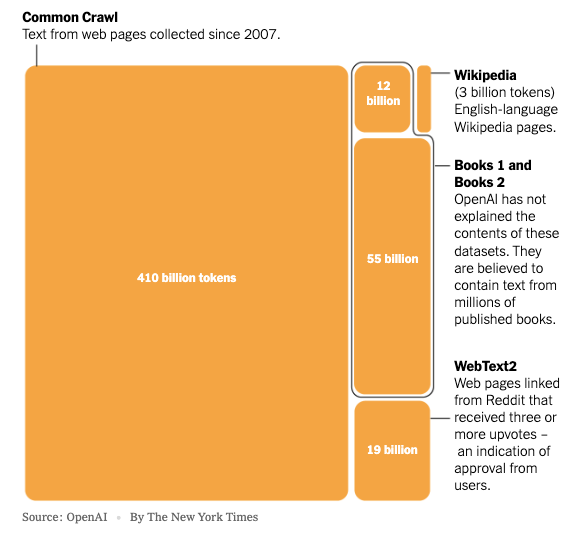
\includegraphics[keepaspectratio]{_resources/images/Ch02-images/OpenAITrainingDataNYTimesChart.png}}

}

\caption{ChatGPT is trained on vast text sources, a distillation of most
human knowledge.}

\end{figure}%

\section{Models Learning from Models: The Recursive Training
Problem}\label{models-learning-from-models-the-recursive-training-problem}

An increasingly troubling issue is the growing proportion of
AI-generated content on the internet. As LLMs produce more and more text
that gets published online, newer models are increasingly training on
outputs from older models rather than authentic human expression. This
creates a recursive problem---models learning from models learning from
models---potentially amplifying biases and errors with each generation.

Researcher Ilia Shumailov at the University of Cambridge calls this
phenomenon ``the curse of recursion,'' and it presents a fundamental
challenge to the current approach of training AI on internet data. As
AI-generated content proliferates, distinguishing authentic human
expression from synthetic text becomes increasingly difficult. This
recursion problem potentially undermines the very foundation of LLM
training by gradually diluting the human element in the training data.

\section{Beyond Text Completion: Fine-Tuning for Specific
Tasks}\label{beyond-text-completion-fine-tuning-for-specific-tasks}

While base LLMs are essentially sophisticated text prediction engines,
they can be adapted for specific purposes through a process called
fine-tuning. This involves additional training on specialized datasets
with human feedback to optimize the model for particular tasks or to
align its outputs with human values.

For example, the base GPT model might generate toxic or harmful content
if that's what the statistical patterns in its training data suggest. To
address this, OpenAI and other companies employ techniques like RLHF
(Reinforcement Learning from Human Feedback), where human evaluators
rate different model outputs, and these ratings are used to further
train the model to produce more helpful, harmless, and honest responses.

This fine-tuning process represents a crucial point of human
intervention in the AI pipeline. The values and judgments of the human
evaluators directly shape what kinds of responses the model will
prioritize. However, this process also introduces new challenges,
including the potential for evaluator biases to become magnified in the
model's behavior and the difficulty of clearly defining concepts like
``helpful'' or ``harmful'' across diverse cultural contexts.

\section{What AI Can't Do: The Limitations That
Matter}\label{what-ai-cant-do-the-limitations-that-matter}

Understanding what LLMs cannot do is as important as appreciating what
they can do. Despite their impressive capabilities, today's AI systems
have several fundamental limitations:

\begin{enumerate}
\def\labelenumi{\arabic{enumi}.}
\item
  \textbf{No Understanding or Consciousness}: LLMs process patterns
  without understanding meaning. They have no consciousness, beliefs,
  desires, or intentions. They cannot truly understand concepts like
  justice, beauty, or truth---they can only mimic how humans talk about
  these concepts.
\item
  \textbf{No Backtracking\index{AI concepts!backtracking} or Planning}:
  As mentioned earlier, LLMs cannot revise earlier parts of their
  generation based on later realizations. They cannot truly plan ahead
  or engage in the kind of recursive thinking that humans employ
  naturally.
\item
  \textbf{No Reality Grounding}: LLMs have no direct access to physical
  reality. Their knowledge comes entirely from text and images in their
  training data, not from embodied experience in the world. They cannot
  verify facts against reality, only against patterns in their training
  data.
\item
  \textbf{No Self-Improvement}: While LLMs can be updated by their
  creators, they cannot improve themselves through experience. Each
  interaction is essentially fresh---the model doesn't learn from its
  mistakes or successes across conversations.
\item
  \textbf{No Originality}: LLMs can combine and recombine elements from
  their training data in new ways, but they cannot create truly original
  concepts. They are fundamentally derivative, limited by what they've
  seen before.
\end{enumerate}

These limitations explain why LLMs, despite their impressive text
generation capabilities, fail at tasks requiring genuine understanding,
counterfactual reasoning, or creative leaps beyond their training data.

\section{The Human Element: What We Bring That AI Can't
Replace}\label{the-human-element-what-we-bring-that-ai-cant-replace}

The limitations of LLMs highlight precisely what makes human
intelligence distinctive and valuable. When we generate language, solve
problems, or make decisions, we do far more than pattern matching. We
understand the world through embodied experience, can plan recursively,
and can imagine counterfactual scenarios. We can backtrack, revise our
thinking, and make creative leaps beyond what we've previously
encountered.

Consider how a skilled financial analyst evaluates an investment
opportunity. They don't simply pattern-match against previous
investments; they consider unique aspects of the current situation,
imagine various future scenarios, and continuously revise their analysis
as new information emerges. They bring judgment based on embodied
experience in the world---something no LLM can replicate.

This is why the most effective applications of AI don't attempt to
replace human judgment but rather to enhance it. When AI handles the
pattern-matching tasks it excels at, humans are freed to focus on the
aspects of work that require judgment, creativity, and understanding.

\section{The Balance: Where Humans and AI
Excel}\label{the-balance-where-humans-and-ai-excel}

The most successful implementations of AI technology recognize the
complementary strengths of humans and machines. AI demonstrates
remarkable capability in processing vast amounts of data quickly and
identifying patterns across large datasets that would overwhelm human
attention. It excels in generating content based on statistical
regularities, performing repetitive tasks with unwavering consistency,
and operating continuously without the fatigue that limits human
performance.

Humans, meanwhile, bring fundamentally different strengths to the table.
We understand context and meaning in ways that transcend statistical
correlation. We make ethical judgments that require balancing competing
values and considering impacts that may not be quantifiable. Our ability
to think recursively and counterfactually---to imagine ``what if''
scenarios and revise our thinking---allows us to navigate novel
situations with a flexibility that AI cannot match. Perhaps most
importantly, humans can create truly novel concepts and approaches, and
adapt to unprecedented situations by drawing on embodied experience and
cross-domain knowledge.

By designing systems that leverage these complementary capabilities,
organizations can achieve outcomes superior to what either humans or AI
could accomplish alone. A human financial analyst with AI assistance,
for instance, can process market data at unprecedented scale while
maintaining the judgment needed to contextualize that data within
broader economic and political realities. This synergy of human and
artificial intelligence is the essence of the
enhancement\index{human-AI relationship!enhancement} thesis we explore
throughout this book.

\section{The Implications: Why This
Matters}\label{the-implications-why-this-matters}

Understanding what AI actually does---and what it doesn't do---has
profound implications for how we implement these technologies in
business and society. When we recognize that LLMs are essentially
sophisticated pattern-matching systems rather than genuinely intelligent
entities, we can make more informed decisions about where and how to
apply them.

This understanding helps explain why purely automated approaches often
disappoint, while enhancement approaches succeed. Automated systems that
attempt to replace human judgment entirely run up against the
fundamental limitations of pattern matching. Enhancement approaches that
combine AI's computational power with human judgment and creativity can
deliver superior results.

For investors, this insight suggests focusing on companies that
understand the complementary nature of human and artificial intelligence
rather than those promising full
automation\index{AI concepts!automation}. For business leaders, it means
designing implementation strategies that augment rather than replace
human capabilities\index{human-AI relationship!human capabilities}. And
for workers, it means developing the distinctively human skills that AI
cannot replicate.

\section{Where We Go From Here}\label{where-we-go-from-here}

As AI technologies continue to advance, the boundary between what they
can and cannot do will shift. Future systems will likely overcome some
of the limitations we've discussed, potentially enabling more
sophisticated reasoning and planning. However, the fundamental
distinction between statistical pattern matching and genuine
understanding remains, and with it, the continued importance of human
judgment.

In the chapters ahead, we'll explore how this understanding of AI's
capabilities and limitations translates into practical implementation
strategies across industries. We'll examine the ``what versus how''
distinction that guides effective human-AI
collaboration\index{human-AI relationship!human-AI collaboration}, the
philosophical dimensions of human judgment, and the investment
implications of the enhancement thesis.

By grounding our approach in a clear-eyed understanding of what AI
actually does, we can move beyond both the hype and the fear to develop
strategies that truly enhance human capabilities rather than attempting
to replace them.

\bookmarksetup{startatroot}

\chapter{The What-How Divide}\label{the-what-how-divide}

AI's Real Impact on Knowledge Work

\hfill\break

Until recently, career success in knowledge work depended heavily on
mastering ``how'' skills - knowing how to build a compelling PowerPoint,
how to structure a financial model, or how to write efficient code. But
as AI systems become more capable at these technical tasks, the
competitive advantage\index{economic!competitive advantage} is shifting
dramatically toward people who know ``what'' needs to be done - those
who can identify the right problems to solve and strategies to pursue.

This fundamental shift from ``how'' to ``what'' has profound
implications for businesses, careers, and investment opportunities.
Let's explore why this transformation is happening and what it means for
different stakeholders.

\section{The Traditional ``How''
Advantage}\label{the-traditional-how-advantage}

Traditionally, organizations needed large teams of specialists who knew
``how'' to perform various technical tasks:

\begin{itemize}
\tightlist
\item
  Financial analysts who knew how to build complex Excel models
\item
  Software engineers who knew how to write code in specific languages
\item
  Designers who knew how to use tools like Photoshop
\item
  Writers who knew how to craft clear technical documentation
\item
  Translators who knew how to convert text between languages
\end{itemize}

These specialists developed their skills through years of practice and
training. Their expertise created both job security and earning power -
companies were willing to pay premium salaries for people who could
execute complex technical tasks effectively.

\section{AI's Disruption of ``How''}\label{ais-disruption-of-how}

Large language models\index{AI concepts!large language models} and other
AI tools are rapidly getting better at many of these ``how'' tasks:

\begin{itemize}
\tightlist
\item
  ChatGPT\index{case studies!ChatGPT} can write basic code in multiple
  languages
\item
  Midjourney can generate sophisticated images
\item
  Translation tools are approaching human-level quality
\item
  AI assistants can create presentations and documentation
\end{itemize}

This capability is expanding quickly. Tasks that seemed immune to
automation\index{AI concepts!automation} just a few years ago are now
being handled competently by AI systems. And unlike human specialists
who may take years to master new skills, AI systems can be rapidly
retrained or fine-tuned for new capabilities.

\section{The Rise of ``What'' Skills}\label{the-rise-of-what-skills}

As AI handles more of the ``how,'' competitive advantage shifts to
people who excel at determining ``what'' needs to be done:

\begin{itemize}
\tightlist
\item
  What problems are worth solving?
\item
  What features should a product include?
\item
  What markets should a company enter?
\item
  What strategies will create sustainable advantages?
\item
  What metrics matter most for success?
\end{itemize}

These ``what'' decisions require capabilities that current AI systems
fundamentally lack:

\textbf{Pattern Recognition\index{AI concepts!pattern recognition}
Across Domains}~Humans can notice subtle patterns and draw insights
across seemingly unrelated fields. A business leader might see parallels
between consumer behavior in fashion and trends in enterprise software,
leading to novel strategic insights. Current AI systems, despite their
broad training, struggle to make these creative connections in
meaningful ways.

\textbf{Judgment Under Uncertainty}~Many crucial business decisions
involve incomplete information and conflicting priorities. Experienced
leaders develop judgment about which risks are worth taking and which
tradeoffs make sense. This type of judgment emerges from years of seeing
both successes and failures firsthand - something AI systems cannot
truly replicate.

\textbf{Understanding Human Context}~Success in business ultimately
depends on understanding human needs, motivations, and behaviors. While
AI can process vast amounts of data about human behavior, it lacks the
innate understanding that comes from being human and experiencing the
full range of human emotions and social dynamics.

\section{Real-World Examples}\label{real-world-examples}

Let's look at some specific examples of how this ``what vs.~how'' divide
plays out:

\subsection{ChatGPT and Chess: The What vs.~How
Divide}\label{chatgpt-and-chess-the-what-vs.-how-divide}

ChatGPT excels at the ``how'' aspects of chess. It can explain rules
with precise clarity, describe tactical motifs like forks and pins,
recommend standard opening principles, and even execute move sequences
when prompted. This ``how'' capability stems from its training on
countless chess books, articles, and game annotations, allowing it to
mimic the instructional patterns of chess literature.

Where ChatGPT fundamentally falls short is in the ``what'' domain of
chess. It cannot determine what strategic approach makes sense in a
complex position, what long-term plan to pursue, or what the most
critical elements of a position are. Even more fundamentally, ChatGPT
cannot decide what it means to ``play chess well'' in the first place.

Consider a simple example: in a given position, should a player
sacrifice material for an attack? This decision requires weighing
potential attacking chances against concrete defensive resources - a
judgment that integrates evaluation of multiple possible futures.
ChatGPT can explain how sacrifices work in general, but cannot reliably
determine what sacrifice (if any) is appropriate in a specific complex
position.

Even more telling is ChatGPT's inability to set appropriate chess goals.
A human must instruct the AI to ``find checkmate in two moves'' or
``evaluate this position'' or ``recommend an opening for a beginner.''
The AI cannot independently determine what chess problems are worth
solving or what chess knowledge would benefit a particular player. It
lacks the purposeful orientation that human players naturally bring to
the game.

This mirrors the broader pattern we've observed across domains. AI
systems like ChatGPT handle the mechanics - the ``how'' - with
impressive competence. But they remain tools awaiting human direction
regarding ``what'' goals to pursue, ``what'' problems need solving, and
``what'' considerations matter most in any given context.

For chess learners, this creates an interesting dynamic. ChatGPT can
serve as an always-available resource for understanding ``how'' chess
pieces move, ``how'' to execute basic tactics, and ``how'' traditional
openings proceed. But determining ``what'' to study, ``what'' skills to
prioritize, and ``what'' strategic approaches align with one's strengths
- these remain distinctly human judgments that no current AI can
meaningfully address.

The limitations become even more apparent in competitive contexts.
Strong human players know that chess is not merely about following rules
and recognizing patterns - it's about making judgments under
uncertainty, having a coherent vision of how the game should develop,
and understanding which factors deserve attention in ambiguous
positions. These ``what'' decisions remain beyond ChatGPT's
capabilities, even as it continues to improve at describing ``how''
chess concepts work in isolation.

As AI capabilities advance, this fundamental divide persists. The most
valuable human contribution isn't executing the mechanical aspects of
chess, but rather making the judgment calls about what matters, what
deserves attention, and what goals are worth pursuing in the first
place.

\subsection{Book-Writing: When Bulldozers Move
Words}\label{book-writing-when-bulldozers-move-words}

What's the value of traditional books when ChatGPT can generate coherent
answers to any question?

A good analogy is with construction projects. Like bulldozers that
efficiently move earth, AI can rapidly generate vast quantities of
coherent text. But just as construction requires both heavy machinery
and skilled artisans, meaningful books need both AI's raw productive
power and human refinement.

However, a well-crafted book offers something different: a carefully
structured approach that helps readers decide their level of engagement.
The finite, constrained nature of a book provides focus that chatbots,
with their endless potential for digression, cannot easily match.

The key to understanding AI's role in authorship lies in recognizing the
distinct phases of book creation.

\begin{enumerate}
\def\labelenumi{\arabic{enumi}.}
\item
  The initial phase - deciding subject matter and scope, aka the
  ``what'' phase --- remains fundamentally human. While AI can help
  brainstorm ideas or identify underexplored topics, the essential
  creative spark and purpose must come from human intention. This
  reflects a broader truth about AI: it excels at processing existing
  patterns but struggles to generate truly novel directions.
\item
  The next phase --- outlining the subject into smaller, related topics
  that make a coherent whole --- demonstrates the potential for human-AI
  collaboration\index{human-AI relationship!human-AI collaboration}. AI
  can quickly generate comprehensive topic structures, but human
  expertise is crucial for identifying gaps, inconsistencies, or areas
  requiring special emphasis. This interplay between AI's broad pattern
  recognition and human domain knowledge creates stronger frameworks
  than either could achieve alone.
\item
  The writing phase is where AI's ``bulldozer'' capabilities shine.
  Instead of laboriously crafting individual sentences, authors can use
  AI to generate substantial blocks of coherent text. This dramatically
  accelerates the initial draft process. However, like rough-graded
  earth, this AI-generated text requires careful refinement to achieve
  its final form.
\item
  The refinement phase is where human
  judgment\index{human-AI relationship!human judgment} becomes
  paramount. Authors must shape the AI-generated content to maintain
  consistent voice, ensure logical flow, and preserve the book's core
  purpose. This requires understanding nuances of audience expectations
  and subject matter that current AI systems cannot fully grasp.
\end{enumerate}

This iterative process of generation and refinement continues until the
project achieves its goals - another judgment that requires human
evaluation. The result is neither purely AI-generated nor traditionally
human-authored, but rather a new form of hybrid creativity that
leverages the strengths of both.

The role of books may evolve, but their fundamental purpose - to present
structured, focused exploration of subjects - will always be valuable.
The challenge for authors is not to compete with AI's raw generative
capabilities, but to use them effectively while maintaining the human
elements that give books their lasting value.

This suggests a future where successful authors are those who master the
art of AI collaboration rather than resist it. Just as modern architects
must understand both traditional design principles and computer-aided
tools, tomorrow's authors will need to balance classic writing skills
with AI capabilities.

The key question is no longer whether AI will replace human authors, but
how it will transform the authorship process. The answer lies in
recognizing that while AI can move mountains of words, humans must still
decide which mountains to move and how to shape the resulting landscape.

This transformation parallels broader changes in knowledge work. As AI
handles more routine cognitive tasks, human value increasingly derives
from higher-order skills like judgment, creativity, and strategic
thinking\index{human-AI relationship!strategic thinking}. The greatest
rewards of authorship, as in many professional fields, will accrue to
those who can effectively combine human insight with AI capabilities.

The rise of AI authors doesn't diminish the value of books but rather
changes how they're created. The essential human elements - purpose,
judgment, refinement - remain crucial, even as AI dramatically expands
our capability to generate and process information. The result may be
not just better books, but new forms of knowledge sharing that we're
only beginning to imagine.

\section{More examples}\label{more-examples}

\subsection{\texorpdfstring{Software
Development\index{software development}: Beyond Code
Generation}{Software Development: Beyond Code Generation}}\label{software-development-beyond-code-generation}

The construction industry provides useful analogies for understanding
AI's impact on software development. Just as modern construction sites
use both automated machinery and skilled human workers, software
development is evolving into a hybrid process where AI handles routine
coding tasks while humans focus on architecture and design decisions.

Think of a typical software project. Traditional development required
writing every line of code manually, like building a house brick by
brick. Now, AI coding assistants like GitHub Copilot or
Amazon\index{case studies!Amazon} CodeWhisperer can generate entire
functions or modules automatically, similar to how prefabricated
components accelerated construction. These AI tools excel at producing
standard elements - authentication systems, database queries, API
endpoints - just as manufacturing\index{manufacturing} automation excels
at producing standardized building materials.

However, like construction projects, software development involves more
than assembling standard components. A successful project requires
understanding user needs, designing intuitive interfaces, ensuring
security, and maintaining long-term reliability. These higher-level
decisions remain firmly in human territory.

The architectural parallel is particularly apt. Just as architects must
consider aesthetics, functionality, and structural integrity, software
architects must balance user experience, system performance, and code
maintainability. AI can suggest implementation details, but it cannot
determine whether a feature aligns with business goals or how it might
affect user behavior.

Technical debt offers another illuminating comparison. In construction,
taking shortcuts (like using lower-grade materials) can speed completion
but creates future maintenance problems. Similarly, in software
development, quick fixes and temporary solutions accumulate as technical
debt. While AI can identify potential debt and suggest refactoring
strategies, humans must weigh the business tradeoffs of addressing it
now versus later.

Integration challenges further highlight AI's limitations. Modern
software systems are complex ecosystems of interacting components, like
cities with interconnected infrastructure systems. AI excels at
optimizing individual components but struggles to understand system-wide
implications. Humans must orchestrate these interactions, ensuring
different parts work together coherently while maintaining system
reliability and performance.

Security considerations demonstrate another crucial human role. Like
building security systems, software security requires anticipating
potential threats and implementing appropriate protections. AI can
identify common vulnerabilities and suggest fixes, but it cannot
understand the broader security context or evaluate risk tradeoffs.
These decisions require human judgment informed by business context and
threat assessment.

The testing and quality assurance phase reveals both AI's strengths and
limitations. AI tools can automatically generate test cases and identify
potential bugs, similar to automated building inspections. However,
human testers are still essential for evaluating user experience,
identifying edge cases, and ensuring the software meets business
requirements. AI can verify that code works as written, but humans must
verify it works as intended.

Looking ahead, successful software development will likely become
increasingly collaborative between humans and AI. Development teams will
need to master new workflows that leverage AI's capabilities while
maintaining human oversight of critical decisions. This might involve
using AI for initial code generation and routine maintenance while
focusing human effort on architecture, security, and user experience.

This evolution parallels broader trends in professional work. Just as
power tools didn't eliminate the need for skilled carpenters but changed
how they work, AI won't eliminate software developers but will transform
their role. The most valuable developers will be those who can
effectively direct AI tools while maintaining high-level system
understanding.

The implications for software education\index{education} and training
are significant. Future developers will need less emphasis on memorizing
syntax and more focus on system design, architecture, and AI
collaboration skills. This mirrors how modern architectural education
focuses less on manual drafting and more on design principles and
computer-aided tools.

However, the fundamental role of human creativity and judgment remains
unchanged. Just as beautiful buildings require human vision despite
advanced construction technology, great software requires human insight
despite sophisticated AI tools. The key is understanding AI as an
enabler of human creativity rather than its replacement. AI working
alone can be competent at creating an adequate building that meets the
programmatic requirements laid out by its developers, but a truly great
building will still require human input and humans' ability to push the
frontier of creativity.

This suggests that software development is entering a new phase where
success depends on effectively combining AI capabilities with human
insight. Here again, the best outcomes will result from humans' ability
to leverage AI. The winners will be those who can best envision how
technology can serve human needs while using AI to implement that vision
efficiently and reliably.

In this new paradigm, the measure of a developer shifts from lines of
code written to the effectiveness of their human-AI collaboration in
creating valuable software solutions. The construction industry's
evolution from manual labor to machine-assisted craftsmanship provides a
roadmap for this transformation.

\subsection{Investment Analysis: Beyond the
Numbers}\label{investment-analysis-beyond-the-numbers}

Just as modern factories use automation for routine manufacturing while
relying on human expertise for product design and quality control,
investment analysis is evolving into a hybrid process where AI handles
data processing while humans focus on strategic insights and judgment
calls.

Let's think of a typical investment analysis project. Traditionally,
analysts spent countless hours gathering financial data, creating
comparison spreadsheets, and writing preliminary reports. Now, AI can
instantly process quarterly reports, generate peer comparisons, and
draft initial analyses. This is similar to how automated assembly lines
handle routine manufacturing tasks, freeing human workers to focus on
complex problems requiring judgment and creativity.

However, like manufacturing, successful investing involves more than
processing standard inputs. While AI excels at identifying patterns in
financial statements and market data, it struggles with crucial
qualitative factors. Can management be trusted? Is the company's
competitive advantage sustainable? Will current market opportunities
persist? These questions require human judgment informed by experience
and industry knowledge.

The manufacturing quality control parallel is particularly relevant.
Just as experienced inspectors can spot subtle defects that automated
systems miss, seasoned investors can identify red flags in management
behavior or market dynamics that AI might overlook. A CEO's body
language during earnings calls, the timing of insider stock sales, or
subtle shifts in competitive dynamics - these nuanced signals often
prove more valuable than quantitative metrics.

Competitive analysis offers another illuminating comparison. In
manufacturing, understanding market dynamics requires more than
analyzing production statistics - it requires insight into changing
consumer preferences, emerging technologies, and competitor strategies.
Similarly, while AI can process vast amounts of market data, humans must
evaluate whether a company's competitive position is truly defensible
and whether management's strategy aligns with market realities.

The role of trust highlights another crucial human element. Just as
manufacturing partnerships require trust built through personal
relationships and demonstrated reliability, investment success often
depends on accurately assessing management credibility. AI can flag
inconsistencies in financial statements or unusual transaction patterns,
but it cannot evaluate character or judge whether explanations for
apparent irregularities are credible.

Market opportunity assessment demonstrates similar limitations. Like
evaluating new manufacturing technologies, assessing market
opportunities requires understanding both technical capabilities and
human behavior. AI can analyze historical market data and identify
trends, but it cannot predict how human customers, competitors, and
regulators will react to new situations. These predictions require human
insight into psychology and social dynamics.

Risk assessment reveals both AI's strengths and limitations. AI systems
can quickly identify common risk factors and calculate standard metrics,
similar to automated safety systems in manufacturing. However, the most
significant risks often come from unexpected directions that don't
appear in historical data. Human judgment remains essential for
identifying and evaluating these non-obvious risks.

Looking ahead, successful investment analysis will likely become
increasingly collaborative between humans and AI. Analysis teams will
need to master new workflows that leverage AI's data processing
capabilities while maintaining human oversight of critical judgments.
This might involve using AI for initial screening and routine monitoring
while focusing human effort on qualitative assessment and strategic
thinking.

This evolution parallels broader trends in professional work. Automation
did not eliminate the need for skilled manufacturing workers but changed
their role, and AI will not eliminate investment analysts but will
transform how they work. The most valuable analysts will be those who
can effectively direct AI tools while maintaining deep industry
understanding and judgment capabilities.

The implications for investment education and training are significant.
Future analysts will need less emphasis on spreadsheet skills and more
focus on business judgment and AI collaboration capabilities. This
mirrors how modern manufacturing education focuses less on manual skills
and more on process management and technology integration.

However, the fundamental role of human judgment remains unchanged. Just
as quality manufacturing requires human oversight despite advanced
automation, successful investing requires human insight despite
sophisticated AI tools. The key is understanding AI as an enhancer of
human judgment rather than its replacement.

This suggests that investment analysis is entering a new phase where
success depends on effectively combining AI capabilities with human
insight. Analysts who can best understand business fundamentals while
using AI will perform better than those who can merely process data
faster.

In this new paradigm, the measure of an analyst shifts from
computational speed to the effectiveness of their human-AI collaboration
in identifying truly attractive investments. The manufacturing
industry's evolution from manual production to technology-enhanced
craftsmanship provides a roadmap for this transformation.

\subsection{\texorpdfstring{AI and Healthcare\index{healthcare}: Beyond
Pattern
Recognition}{AI and Healthcare: Beyond Pattern Recognition}}\label{ai-and-healthcare-beyond-pattern-recognition}

The evolution of AI in healthcare parallels modern manufacturing quality
control, where automated systems handle routine inspections while
skilled technicians focus on complex problems requiring human judgment.
Similarly, healthcare is becoming a hybrid system where AI processes
medical data while human doctors focus on patient relationships and
complex medical decisions.

Consider a typical diagnostic process. Traditionally, doctors spent
considerable time reviewing test results, consulting medical literature,
and documenting findings. Now, AI can instantly analyze lab results,
medical images, and patient histories to suggest potential diagnoses.
This is similar to how automated inspection systems quickly identify
defects in manufactured products, allowing human inspectors to focus on
more complex quality issues.

However, like quality control, successful healthcare involves more than
pattern recognition. While AI excels at identifying anomalies in test
results and suggesting standard treatments, it struggles with crucial
contextual factors. How will a patient's living situation affect
treatment adherence? Which side effects are acceptable given a patient's
lifestyle? What treatment modifications are needed given other health
conditions? These questions require human judgment informed by direct
patient interaction and medical experience.

The empathy factor is particularly relevant. Effective quality control
requires understanding how products will be used in real-world
conditions, and effective healthcare requires understanding patients'
lives and concerns. AI can process medical histories and suggest
treatment protocols, but it cannot truly empathize with patient fears or
understand how cultural and personal factors might affect treatment
success.

Treatment customization offers another illuminating comparison. In
manufacturing, standard quality metrics must often be adjusted for
specific use cases. Similarly, while AI can recommend standard
treatments based on medical literature, doctors must adapt these
recommendations to individual patient circumstances. A treatment
protocol that looks optimal on paper might be impractical or
inappropriate given a patient's specific situation.

The trust relationship highlights another crucial human element. In the
same way that manufacturing quality depends on trust between suppliers
and customers, healthcare outcomes often depend on patient trust in
their medical providers. AI can provide accurate medical information,
but it cannot build the personal trust that encourages treatment
compliance and honest symptom reporting.

Emergency response demonstrates both AI's strengths and limitations. AI
systems can quickly process vital signs and suggest immediate
interventions, similar to automated safety systems in manufacturing.
However, emergency medicine often requires split-second decisions based
on incomplete information and complex tradeoffs. Human judgment remains
essential for these high-stakes decisions where standard protocols may
not apply.

Looking ahead, successful healthcare will likely become increasingly
collaborative between humans and AI. Medical teams will need to master
new workflows that leverage AI's analytical capabilities while
maintaining human oversight of critical decisions. This might involve
using AI for initial screening and routine monitoring while focusing
human effort on patient interaction and complex case management.

This evolution parallels broader trends in professional work. Automation
did not eliminate the need for skilled quality control technicians but
changed their role, and AI will not eliminate doctors but will transform
how they work. The most valuable healthcare providers will be those who
can effectively direct AI tools while maintaining strong patient
relationships and clinical judgment.

The implications for medical education and training are significant.
Future doctors will need less emphasis on memorizing medical facts and
more focus on patient communication and AI collaboration skills. This
mirrors how modern quality control training focuses less on inspection
procedures and more on system management and problem-solving.

However, the fundamental role of human judgment remains unchanged.
Quality control requires human oversight despite advanced inspection
technology, and healthcare requires human insight despite sophisticated
AI tools. The key is understanding AI as an enhancer of medical judgment
rather than its replacement.

This suggests that healthcare is entering a new phase where success
depends on effectively combining AI capabilities with human insight.
Those who can understand patient needs while using AI to enhance this
understanding will reap more rewards than those who can merely recall
the most medical facts and procedures.

In this new paradigm, the measure of a healthcare provider shifts from
diagnostic speed to the effectiveness of their human-AI collaboration in
achieving optimal patient outcomes. The quality control industry's
evolution from manual inspection to technology-enhanced oversight
provides a roadmap for this transformation.

The challenge ahead is not whether to adopt AI in healthcare, but how to
integrate it while preserving the human elements that make medicine
effective. Success will require understanding both AI's capabilities and
its limitations, while never losing sight of healthcare's fundamental
mission: helping human patients achieve better health outcomes through
personalized, compassionate care.

\section{Investment Implications}\label{investment-implications}

For investors, the what-how framework offers valuable guidance for
evaluating AI-related opportunities. Companies positioned to win in this
environment include those that:

\begin{enumerate}
\def\labelenumi{\arabic{enumi}.}
\tightlist
\item
  Develop tools that enhance human strategic thinking rather than merely
  automating implementation tasks.
\item
  Create platforms that facilitate seamless collaboration between human
  judgment and AI execution.
\item
  Build solutions that maintain appropriate human oversight while
  leveraging AI capabilities.
\item
  Design business models that recognize and reward uniquely human
  contributions.
\end{enumerate}

By contrast, companies that focus exclusively on automation without
considering the continued importance of human judgment will likely
struggle to deliver sustainable value. The most successful AI
implementations will be those that augment rather than replace human
capabilities\index{human-AI relationship!human capabilities}, allowing
people to focus on the high-value what decisions where they maintain a
durable advantage.

This perspective offers a useful corrective to the common investor
tendency to overvalue pure automation plays. The history of technology
adoption suggests that approaches that enhance rather than replace human
capabilities typically deliver more sustainable value over time.

\section{The Evolution of Knowledge
Work}\label{the-evolution-of-knowledge-work}

As AI capabilities continue to evolve, we can anticipate further shifts
in the relative value of different forms of human contribution.
Implementation skills---the \emph{how}---will continue to be
commoditized, while strategic judgment---the \emph{what}---will command
an increasing premium. This doesn't mean implementation expertise
becomes irrelevant, but rather that it must be paired with higher-level
strategic capabilities to remain valuable.

For individual knowledge workers, this suggests a clear direction for
professional development. Rather than focusing exclusively on technical
mastery within narrow domains, sustainable career advancement will
require developing broader strategic capabilities: understanding
stakeholder needs, synthesizing insights across disciplines, and making
nuanced judgments that integrate technical, business, and ethical
considerations.

For educational institutions, the what-how divide suggests the need for
fundamental curriculum redesign. Traditional education systems heavily
emphasize \emph{how} skills---teaching specific methodologies, tools,
and techniques. Future-oriented education should place greater emphasis
on developing students' abilities to frame problems effectively, think
across disciplinary boundaries, and make contextual judgments that
cannot be easily automated.

For policymakers, this framework offers a more nuanced understanding of
AI's impact on employment and economic opportunity. Rather than focusing
exclusively on potential job displacement, policy approaches should
consider how to facilitate the transition toward work that emphasizes
uniquely human strategic capabilities while ensuring that the benefits
of AI-driven productivity gains are broadly shared.

\section{\texorpdfstring{Integration with
Enhancement\index{human-AI relationship!enhancement}
Thesis}{Integration with Enhancement Thesis}}\label{integration-with-enhancement-thesis}

The what-how framework aligns perfectly with our core thesis that AI
will enhance rather than replace human capabilities across industries.
By automating routine implementation tasks, AI frees human cognitive
capacity for higher-level strategic thinking---the domain where human
judgment maintains a durable advantage. This represents not replacement
but enhancement of human potential.

This perspective also explains why purely automated approaches often
disappoint. When AI systems operate without appropriate human direction
and oversight, they may execute flawlessly within their
parameters\index{AI concepts!parameters} while completely missing the
broader context that gives their outputs meaning and value. The most
successful implementations maintain humans ``in the loop'' precisely
because human judgment about what matters cannot be delegated to
automated systems.

In the case of full self-driving technology, which we'll explore more
fully in later chapters, companies like Tesla\index{case studies!Tesla}
have collected unprecedented amounts of driving data and developed
increasingly sophisticated systems for navigating complex environments.
Yet as robotics pioneer Rodney Brooks has observed, these systems still
struggle with the contextual judgment that experienced human drivers
exercise effortlessly.

A human driver approaching a neighborhood with cars parked tightly on
both sides naturally slows down, recognizing the increased risk of
children darting into the street. This judgment doesn't derive from
explicit rules but from a holistic understanding of context that
integrates multiple factors---some explicit, others tacit. Autonomous
systems may eventually replicate this behavior through sophisticated
pattern recognition, but they cannot independently determine which
factors deserve attention without human direction.

\section{Conclusion: Navigating the
Transformation}\label{conclusion-navigating-the-transformation}

The what-how divide provides a powerful framework for understanding AI's
true impact on knowledge work and business strategy. Rather than
wholesale replacement, we're witnessing a fundamental shift in the
nature of human contribution---from executing well-defined tasks to
making strategic judgments about what deserves attention and how
different considerations should be weighed.

This transformation presents both challenges and opportunities.
Organizations and individuals that continue to focus exclusively on
implementation skills will find their competitive position eroding as AI
systems increasingly automate these functions. Those who develop the
strategic judgment to determine what is worth doing---and the ability to
direct AI systems effectively toward these ends---will thrive in an
AI-enhanced economy.

The what-how framework aligns with our broader thesis that successful AI
implementation requires keeping humans ``in the loop.'' Not because of
temporary technical limitations that will eventually be overcome, but
because of fundamental differences between human and artificial
intelligence\index{AI concepts!artificial intelligence}. The most
valuable human contributions have always involved more than technical
execution---they reflect purpose, meaning, and judgment that remain
uniquely human even as AI capabilities advance.

In the next chapter, we'll explore these philosophical dimensions more
deeply, examining why understanding the nature of human intelligence is
crucial for designing effective human-AI collaborations. By recognizing
both the capabilities and limitations of artificial intelligence, we can
develop approaches that truly enhance human potential rather than
attempting to replace it.

\begin{figure}

\centering{

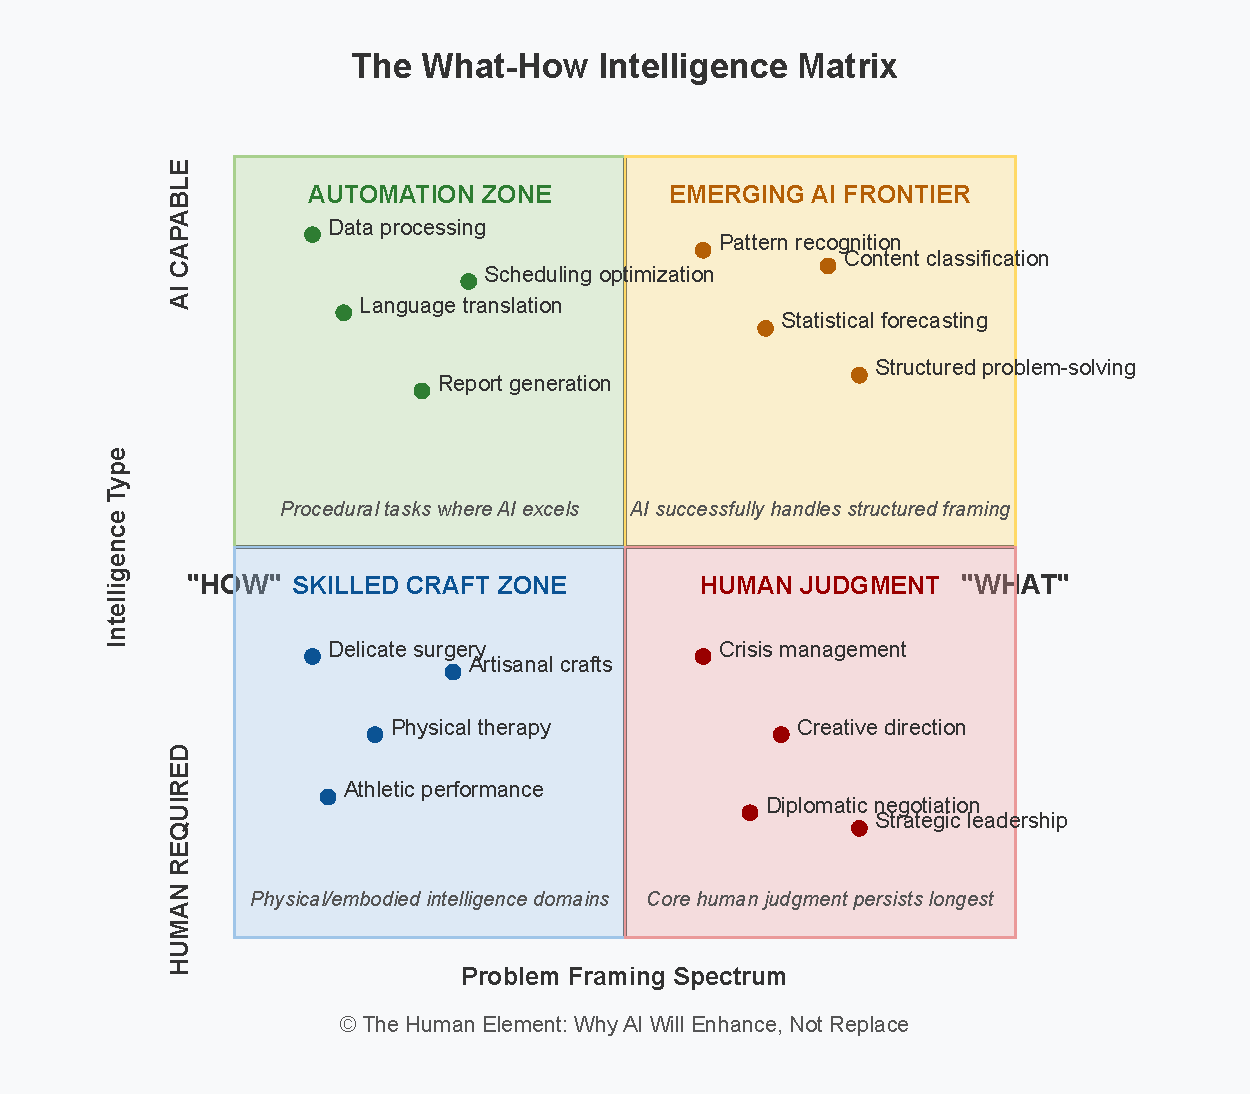
\includegraphics[width=0.95\linewidth,height=\textheight,keepaspectratio]{index_files/mediabag/_resources/images/Ch03-images/what-how-matrix.pdf}

}

\caption{\label{fig-what-how-matrix}What-How Matrix}

\end{figure}%

\section{Beyond the False Binary}\label{beyond-the-false-binary}

The current discourse on AI's impact falls into a tiresome and
inaccurate binary: either AI will replace human workers entirely, or its
effects will be marginal. Both narratives miss the fundamental
transformation underway. What we're witnessing is not wholesale
replacement but a profound shift in the nature of human contribution---a
redistribution of value across the knowledge work spectrum that
redefines which human capabilities command a premium.

This transformation becomes apparent when we distinguish between two
fundamental aspects of any intellectual task: determining \emph{what}
needs to be done versus executing \emph{how} to do it. This distinction,
while seemingly straightforward, carries profound implications for the
future of work\index{policy!future of work}, business strategy, and
investment that extend far beyond the simplistic replacement narrative
dominating public discourse.

The what-how framework offers remarkable clarity amid the confusing
narratives surrounding AI. It helps explain why certain cognitive tasks
are rapidly becoming commoditized while others remain stubbornly
resistant to automation. More importantly, it provides a roadmap for
individuals, organizations, and policymakers navigating a landscape
where artificial intelligence increasingly pervades knowledge work.

Until the arrival of generative AI\index{AI concepts!generative AI},
individuals gained professional advantages through superior ``how''
skills---they excelled at crafting compelling presentations, building
complex spreadsheets, writing efficient code, or translating between
languages. These implementation abilities represented valuable skills
that could be developed and applied on behalf of those who
determined~\emph{what}~needed to be done.

In traditional organizational hierarchies, executives and managers
typically decide~\emph{what}~initiatives to pursue, while specialized
knowledge workers determine~\emph{how}~to execute them. This division
has historically functioned efficiently
because~\emph{how}~expertise---whether in financial modeling, software
development, or content creation\index{content creation}---required
significant investment in learning specialized tools and methodologies.

The emergence of sophisticated AI systems fundamentally alters this
equation. Large language models demonstrate remarkable proficiency in
implementation tasks, often exceeding human capabilities in narrow
domains. They can generate code, compose business communications, create
visual assets, and perform complex analyses with minimal human guidance.
These systems excel precisely in the domain of~\emph{how}---the
execution of well-defined tasks within established parameters.

What these systems cannot do---and what remains uniquely human---is
determine~\emph{what}~is worth doing in the first place. They cannot
independently identify which problems merit attention, which strategies
align with organizational values, or which approaches will resonate with
stakeholders. They lack the contextual
understanding\index{human-AI relationship!contextual understanding},
ethical framework, and strategic vision required to make these
determinations.

As noted already, the financial analyst traditionally created value from
technical modeling skills. As AI systems increasingly automate complex
financial calculations, the analyst's competitive advantage shifts
toward identifying which factors merit analysis, which comparisons yield
strategic insights, and how findings translate into investment
decisions. The technical implementation---the~\emph{how}---becomes
commoditized, while judgment about~\emph{what}~to analyze becomes the
primary value driver.

This pattern repeats across knowledge work domains. In
marketing\index{marketing}, AI can generate endless variations of
campaign materials, but cannot determine which messaging will align with
brand values and audience expectations. In software development, AI can
produce functional code based on specifications but cannot identify
which features will deliver genuine user value. In healthcare, AI can
analyze diagnostic images with remarkable accuracy but cannot integrate
these findings with the full context of patient well-being.

\section{Philosophical Dimensions of the
Divide}\label{philosophical-dimensions-of-the-divide}

The what-how divide resonates with deeper philosophical questions about
the nature of intelligence and agency. Martin
Heidegger\index{philosophy!Heidegger}, whose work we explore more fully
in Chapter 4, offers particularly relevant insights through his concept
of ``comportments''---the way humans face and engage with the world
around them.

When we are deeply engaged in an activity---skillfully driving a car,
playing an instrument, or writing code---we are not consciously thinking
about the mechanics of these actions. Our focus extends beyond the
immediate task to its purpose and meaning within our broader existence.
The ultimate comportment\index{philosophy!Heidegger!comportment},
Heidegger suggests, is our orientation toward being itself, which
encompasses our understanding of past, present, and future.

Artificial intelligence systems, even sophisticated ones like GPT-4 or
Claude, lack these comportments. They process information without any
inherent purpose or temporal orientation. They can mimic human-like
outputs but have no concept of why these outputs matter or how they fit
into broader human concerns. This philosophical distinction manifests
practically in AI's inability to determine \emph{what} is worth doing
independent of human direction.

The what-how divide thus represents more than a practical delineation of
tasks; it reflects a fundamental distinction between human and
artificial intelligence. While AI excels at executing well-defined
processes---the \emph{how}---it cannot engage with the existential
questions of purpose and meaning that inform human decisions about
\emph{what} deserves attention.

This philosophical perspective helps explain why LLMs struggle with
certain seemingly simple tasks, as we demonstrated in prior chapters.
Tasks that require constant re-evaluation and adjustment based on
evolving goals---like writing a sentence that accurately describes its
own length or completing a Sudoku puzzle---reveal the fundamental
limitations of systems that cannot backtrack or reconsider their
approach once they've begun generating outputs.

\section{Case Studies: The Divide in
Practice}\label{case-studies-the-divide-in-practice}

To illustrate the what-how divide, let's examine several domains where
this transformation is particularly evident:

\subsection{Software Development}\label{software-development}

Traditional programming expertise focused heavily on implementation
details---mastering specific languages, frameworks, and architectural
patterns. While these technical skills remain valuable, AI code
generation tools increasingly automate routine implementation tasks. The
premium shifts toward determining which features will deliver value, how
systems should interact with users, and what architectural decisions
will support long-term business objectives.

Senior developers report that junior programmers who once spent years
mastering syntax and debugging techniques now leverage AI assistants to
handle these aspects, allowing them to focus earlier in their careers on
higher-level system design and user experience
considerations---traditionally the domain of more experienced
developers.

This shift alters the career progression trajectory for software
engineers. Technical implementation skills remain necessary but
insufficient; they must be paired with strategic judgment about what
deserves implementation in the first place. Engineers who maintain
purely technical focus without developing this broader perspective may
find their competitive position eroding as AI systems increasingly
automate routine coding tasks.

\subsection{Content Creation}\label{content-creation}

In media and marketing, AI systems now generate remarkably coherent and
stylistically appropriate content at scale. The limiting factor is no
longer production capacity but strategic direction---determining which
messages will resonate with target audiences, which topics deserve
attention, and how content aligns with broader brand narratives.

Marketing executives evaluating AI writing assistants frequently report
that while these tools can ``automatically compose email replies,''
users typically spend as much time editing these drafts as they would
creating responses from scratch. The real value emerges when humans with
deep customer knowledge direct these tools toward specific strategic
objectives.

This transformation extends beyond business communication to creative
fields. As we explored with the AI-generated completion of
Beethoven\index{Beethoven}'s unfinished tenth symphony, technical
proficiency alone cannot replicate the ineffable quality that
distinguishes truly meaningful creative work. As music critic Jan
Swafford observed, ``We humans need to see the human doing it.'' The
value derives not just from the output itself but from knowing it
represents authentic human struggle, insight, and purpose.

\subsection{Healthcare}\label{healthcare}

Medical diagnostic systems increasingly match or exceed human
performance in analyzing medical images, identifying patterns in patient
data, and suggesting potential diagnoses. Yet these systems cannot
determine which factors are most relevant for a particular patient, how
to weigh complex trade-offs between treatment options, or how to
communicate findings in ways that respect patient values and
preferences.

A physician whose only skill is knowing \emph{how} to diagnose a
patient's condition is becoming less necessary. The crucial human
contribution shifts toward determining \emph{what} aspects of patient
wellbeing deserve priority, which treatment approaches align with
patient values, and how to integrate medical insights with broader
quality-of-life considerations.

This shift carries significant implications for medical education and
practice. Technical diagnostic skills remain essential but must
increasingly be paired with heightened capabilities for integrative
judgment, ethical reasoning, and communication. The most effective
healthcare practitioners of the future will leverage AI for routine
analytical tasks while focusing their human expertise on the complex
judgments that machines cannot make.

\section{The Competitive Dynamics of the
Divide}\label{the-competitive-dynamics-of-the-divide}

The what-how framework carries significant implications for competitive
strategy across industries. As implementation capabilities become
increasingly commoditized through AI, sustainable competitive advantage
shifts toward superior judgment about what deserves implementation in
the first place.

This dynamic particularly challenges organizations that have
traditionally derived their advantage primarily from superior execution.
When AI systems can implement strategies with comparable efficiency
across competitors, the primary differentiator becomes the quality of
strategic judgment guiding that implementation. Organizations must
evolve their capabilities accordingly, developing institutional capacity
for the complex judgments that remain resistant to automation.

We see this pattern emerging in investment
management\index{investment management}, where quantitative analysis
tools have become increasingly sophisticated and widely available. The
differentiator for successful investment firms shifts toward superior
judgment about which factors merit analysis, which market signals
deserve attention, and how various considerations should be weighted in
decision-making\index{AI concepts!decision-making}.

Similarly, in management consulting, the technical aspects of data
analysis and presentation---traditionally key components of the service
offering---are increasingly automated. The value proposition shifts
toward helping clients determine which problems deserve attention, which
approaches align with organizational values, and how various factors
should be prioritized.

For technology companies specifically, the what-how framework offers
valuable guidance for product development. The most successful AI
implementations enhance rather than replace human judgment, allowing
people to focus on the high-value \emph{what} decisions where they
maintain a durable advantage. Products that merely automate
implementation without facilitating better strategic decisions will
struggle to deliver sustainable value.

\section{Organizational Implications}\label{organizational-implications}

This fundamental shift carries significant implications for how
organizations approach talent development, operational structure, and
competitive strategy. Companies that recognize and adapt to the what-how
divide will establish sustainable advantages in an AI-enhanced economy.

First, talent development programs must evolve beyond technical training
focused on implementation skills. While baseline technical literacy
remains essential, organizations should invest more heavily in
developing employees' abilities to frame problems effectively,
synthesize insights across domains, and make nuanced judgments that
integrate technical, business, and ethical considerations.

The most valuable professional development initiatives will foster
precisely those capabilities that remain distinctly human---contextual
understanding, strategic synthesis, and ethical judgment. This
represents a significant departure from traditional approaches that
emphasize mastery of specific tools and methodologies.

Second, workflow design should consciously separate strategic decisions
from implementation details, creating clear interfaces between human
judgment and AI execution. This approach maintains appropriate human
oversight while leveraging AI's capabilities for rapid, consistent
implementation.

Effective workflow design requires careful consideration of where human
judgment adds the most value. Rather than automating entire processes
end-to-end, organizations should identify the critical decision points
where human judgment remains essential and design workflows that
explicitly incorporate this judgment while automating surrounding
implementation steps.

Third, organizational structures should evolve to emphasize roles that
combine domain expertise with AI
literacy\index{implementation!AI literacy}. The traditional separation
between business strategists and technical implementers becomes less
valuable as AI systems increasingly bridge this gap. New hybrid roles
will emerge that focus on translating business objectives into effective
AI implementation approaches.

This structural evolution may require reconsidering traditional career
paths and reporting relationships. Organizations that maintain rigid
distinctions between technical and strategic roles may struggle to
develop the integrated capabilities needed for effective human-AI
collaboration.

\section{Investment Implications}\label{investment-implications-1}

For investors, the what-how framework offers valuable guidance for
evaluating AI-related opportunities. Companies positioned to win in this
environment include those that:

\begin{enumerate}
\def\labelenumi{\arabic{enumi}.}
\tightlist
\item
  Develop tools that enhance human strategic thinking rather than merely
  automating implementation tasks.
\item
  Create platforms that facilitate seamless collaboration between human
  judgment and AI execution.
\item
  Build solutions that maintain appropriate human oversight while
  leveraging AI capabilities.
\item
  Design business models that recognize and reward uniquely human
  contributions
\end{enumerate}

By contrast, companies that focus exclusively on automation without
considering the continued importance of human judgment will likely
struggle to deliver sustainable value. The most successful AI
implementations will be those that augment rather than replace human
capabilities, allowing people to focus on the high-value \emph{what}
decisions where they maintain a durable advantage.

This perspective offers a useful corrective to the common investor
tendency to overvalue pure automation plays. The history of technology
adoption suggests that approaches that enhance rather than replace human
capabilities typically deliver more sustainable value over time.

\section{The Evolution of Knowledge
Work}\label{the-evolution-of-knowledge-work-1}

As AI capabilities continue to evolve, we can anticipate further shifts
in the relative value of different forms of human contribution.
Implementation skills---the \emph{how}---will continue to be
commoditized, while strategic judgment---the \emph{what}---will command
an increasing premium. This doesn't mean implementation expertise
becomes irrelevant, but rather that it must be paired with higher-level
strategic capabilities to remain valuable.

For individual knowledge workers, this suggests a clear direction for
professional development. Rather than focusing exclusively on technical
mastery within narrow domains, sustainable career advancement will
require developing broader strategic capabilities: understanding
stakeholder needs, synthesizing insights across disciplines, and making
nuanced judgments that integrate technical, business, and ethical
considerations.

For educational institutions, the what-how divide suggests the need for
fundamental curriculum redesign. Traditional education systems heavily
emphasize \emph{how} skills---teaching specific methodologies, tools,
and techniques. Future-oriented education should place greater emphasis
on developing students' abilities to frame problems effectively, think
across disciplinary boundaries, and make contextual judgments that
cannot be easily automated.

For policymakers, this framework offers a more nuanced understanding of
AI's impact on employment and economic opportunity. Rather than focusing
exclusively on potential job displacement, policy approaches should
consider how to facilitate the transition toward work that emphasizes
uniquely human strategic capabilities while ensuring that the benefits
of AI-driven productivity gains are broadly shared.

\section{Integration with Enhancement
Thesis}\label{integration-with-enhancement-thesis-1}

The what-how framework aligns perfectly with our core thesis that AI
will enhance rather than replace human capabilities across industries.
By automating routine implementation tasks, AI frees human cognitive
capacity for higher-level strategic thinking---the domain where human
judgment maintains a durable advantage. This represents not replacement
but enhancement of human potential.

This perspective also explains why purely automated approaches often
disappoint. When AI systems operate without appropriate human direction
and oversight, they may execute flawlessly within their parameters while
completely missing the broader context that gives their outputs meaning
and value. The most successful implementations maintain humans ``in the
loop'' precisely because human judgment about \emph{what} matters cannot
be delegated to automated systems.

In the case of full self-driving technology, which we'll explore more
fully in later chapters, companies like Tesla have collected
unprecedented amounts of driving data and developed increasingly
sophisticated systems for navigating complex environments. Yet as
robotics pioneer Rodney Brooks has observed, these systems still
struggle with the contextual judgment that experienced human drivers
exercise effortlessly.

A human driver approaching a neighborhood with cars parked tightly on
both sides naturally slows down, recognizing the increased risk of
children darting into the street. This judgment doesn't derive from
explicit rules but from a holistic understanding of context that
integrates multiple factors---some explicit, others tacit. Autonomous
systems may eventually replicate this behavior through sophisticated
pattern recognition, but they cannot independently determine which
factors deserve attention without human direction.

\section{Conclusion: Navigating the
Transformation}\label{conclusion-navigating-the-transformation-1}

The what-how divide provides a powerful framework for understanding AI's
true impact on knowledge work and business strategy. Rather than
wholesale replacement, we're witnessing a fundamental shift in the
nature of human contribution---from executing well-defined tasks to
making strategic judgments about what deserves attention and how
different considerations should be weighed.

This transformation presents both challenges and opportunities.
Organizations and individuals that continue to focus exclusively on
implementation skills will find their competitive position eroding as AI
systems increasingly automate these functions. Those who develop the
strategic judgment to determine \emph{what} is worth doing---and the
ability to direct AI systems effectively toward these ends---will thrive
in an AI-enhanced economy.

The what-how framework aligns with our broader thesis that successful AI
implementation requires keeping humans ``in the loop.'' Not because of
temporary technical limitations that will eventually be overcome, but
because of fundamental differences between human and artificial
intelligence. The most valuable human contributions have always involved
more than technical execution---they reflect purpose, meaning, and
judgment that remain uniquely human even as AI capabilities advance.

In the next chapter, we'll explore these philosophical dimensions more
deeply, examining why understanding the nature of human intelligence is
crucial for designing effective human-AI collaborations. By recognizing
both the capabilities and limitations of artificial intelligence, we can
develop approaches that truly enhance human potential rather than
attempting to replace it.

\bookmarksetup{startatroot}

\chapter{Beyond Computation: The Philosophy of Human
Intelligence}\label{beyond-computation-the-philosophy-of-human-intelligence}

What Heidegger and other thinkers reveal about the fundamental
differences between human and artificial intelligence

\hfill\break

Previous chapters examined AI's capabilities and limitations from
technical and business perspectives. But to truly understand why human
intelligence remains irreplaceable, we need to explore the philosophical
underpinnings of intelligence itself. This requires venturing beyond the
dominant analytical tradition of Anglo-American philosophy---with its
focus on logic, language, and computation---into Continental philosophy,
where thinkers like Martin Heidegger\index{philosophy!Heidegger},
Maurice Merleau-Ponty, and Jean-Paul Sartre grappled more directly with
questions of being, consciousness, and embodied existence.

The prevailing narrative of artificial
intelligence\index{AI concepts!artificial intelligence} rests on a
fundamental assumption inherited from Descartes: that intelligence is
essentially computational. Descartes' famous declaration, ``I think,
therefore I am,'' positioned abstract reasoning as the defining
characteristic of human existence. This Cartesian model frames the mind
as a thinking mechanism separate from both body and world---a
disembodied processor of information. The modern project of artificial
intelligence follows directly from this conception: if human
intelligence is fundamentally computational, then creating artificial
intelligence simply requires building sufficiently sophisticated
computational systems.

But what if this foundational assumption is wrong? What if human
intelligence isn't primarily computational at all, but emerges from our
embodied, situated existence in the world? This is precisely the
argument advanced by Heidegger and other Continental philosophers, and
it is critical to our understanding of both human and artificial
intelligence.

\section{\texorpdfstring{Being-in-the-World\index{philosophy!Heidegger!being-in-the-world}:
Heidegger's Fundamental
Insight}{Being-in-the-World: Heidegger's Fundamental Insight}}\label{being-in-the-world-heideggers-fundamental-insight}

Heidegger's masterwork,~\emph{Being and Time}~(1927), represents a
radical departure from the Cartesian tradition. Where Descartes begins
with the isolated, thinking subject, Heidegger starts with what he
calls~\emph{Dasein\index{philosophy!Heidegger!Dasein}}~(literally
``being-there'')---human existence characterized by its fundamental
embeddedness in a meaningful world. For Heidegger, we are not primarily
thinking beings who sometimes act in the world; we are fundamentally
beings-in-the-world who occasionally step back to think abstractly.

This distinction may seem subtle, but its implications are profound. In
the Cartesian model, our primary relationship to the world is one of
detached observation and calculation---we represent the world internally
and then compute appropriate responses. In Heidegger's model, our
primary relationship to the world is one of practical engagement---we
are always already involved in meaningful situations that shape our
perceptions, actions, and understanding.

Let's see how this plays out in skilled performance. A virtuoso pianist
doesn't mentally represent each note before playing it; she is absorbed
in the activity itself, responding fluidly to the music as it unfolds. A
seasoned trader doesn't consciously calculate each market move; he
intuitively reads patterns and responds with practiced expertise.
Heidegger describes this mode of engagement as
``ready-to-hand\index{philosophy!Heidegger!ready-to-hand}''
(\emph{Zuhandenheit})---a state where tools and skills become extensions
of ourselves rather than objects of conscious attention.

This ready-to-hand mode contrasts sharply with what Heidegger calls
``present-at-hand\index{philosophy!Heidegger!present-at-hand}''
(\emph{Vorhandenheit})---the detached, analytical stance we adopt when
something breaks down or becomes problematic. When the pianist hits a
wrong note or the trader encounters an anomalous market pattern, they
shift from absorbed engagement to conscious analysis. This analytical
stance approximates the Cartesian model of detached representation, but
for Heidegger, it's a derived and secondary mode of engagement, not our
primary way of being in the world.

\section{Implications for Artificial
Intelligence}\label{implications-for-artificial-intelligence}

This philosophical reframing has profound implications for artificial
intelligence. Current AI systems---even sophisticated ones like large
language models\index{AI concepts!large language models}---operate
entirely in the ``present-at-hand'' mode. They process information,
identify patterns, and generate outputs based on statistical
correlations, but they lack the capacity for ``ready-to-hand''
engagement with the world.

This limitation becomes apparent when we examine the capabilities and
limitations of current AI systems. Recall the example from earlier
chapters: large language models cannot ``backtrack'' or revise their
fundamental assumptions mid-stream. When tasked with writing ``a
sentence that describes its own length in words,'' they consistently
fail despite their impressive pattern-recognition capabilities. This
isn't merely a technical limitation that future iterations will
overcome; it reflects a more fundamental difference between
computational processing and human understanding.

Human understanding emerges from our practical engagement with the
world---what Heidegger calls our ``pre-understanding'' or
``fore-structure of understanding.'' We always approach situations with
a tacit grasp of how things work, gained through our embodied experience
in a shared world of meaning. This pre-understanding isn't represented
explicitly in propositional form; it's woven into our very way of being
in the world.

AI systems lack this pre-understanding because they don't inhabit the
world as we do. They process information but don't experience it in a
meaningful context. This explains why AI systems can process vast
amounts of text about human emotions without ever feeling them, or
analyze countless images of objects without developing a practical
understanding of how those objects function in everyday life.

\section{Temporality and Human
Understanding}\label{temporality-and-human-understanding}

Heidegger further distinguishes human intelligence through his concept
of temporality. For Heidegger, humans exist temporally---our
understanding of the present is always shaped by our experience of the
past and our projection toward the future. This temporal structure isn't
merely about placing events on a timeline; it's about how past, present,
and future interpenetrate in our lived experience.

When a skilled investor makes decisions, he isn't simply processing
current data; he's drawing on his lived experience of past market cycles
and projecting potential futures based on that understanding. This
temporality isn't reducible to a database of past events plus a
prediction algorithm. It's a unified structure of experience that shapes
how the investor perceives and interprets the present.

AI systems, in contrast, can process historical data and make
statistical projections, but they lack this unified temporal structure.
Their ``knowledge'' of the past consists of statistical patterns
extracted from training data\index{AI concepts!training data}, not lived
experience. Their projections of the future derive from these same
patterns, not from a meaningful engagement with possibilities that
matter to them. This difference becomes particularly evident in novel
situations that diverge significantly from historical
patterns---precisely the situations where human
judgment\index{human-AI relationship!human judgment} proves most
valuable.

\section{The Social Dimension of
Intelligence}\label{the-social-dimension-of-intelligence}

Another crucial aspect of human intelligence emerges from what Heidegger
calls ``being-with'' (\emph{Mitsein})---our fundamental connectedness
with other humans in a shared world of meaning. Human intelligence
develops through social interaction, cultural inheritance, and
participation in what philosopher Hans-Georg Gadamer later called
``traditions of understanding.''

Consider how a seasoned executive can ``read the room'' during a complex
negotiation. This capacity isn't merely about processing verbal
statements and visual cues; it draws on a lifetime of social and
cultural understanding that allows the executive to sense tensions,
identify shared interests, and navigate complex human dynamics. This
social intelligence emerges from our participation in a shared world of
meaning that AI systems, despite their sophisticated pattern
recognition\index{AI concepts!pattern recognition} capabilities, don't
inhabit.

This social dimension helps explain why AI systems trained on internet
text often reproduce biases, stereotypes, and problematic patterns
present in their training data. These systems don't possess the social
understanding that allows humans to critically evaluate cultural norms
and practices. They can mimic patterns of language without grasping the
ethical and social implications of those patterns.

\section{\texorpdfstring{The Case for
Enhancement\index{human-AI relationship!enhancement} Rather Than
Replacement}{The Case for Enhancement Rather Than Replacement}}\label{the-case-for-enhancement-rather-than-replacement}

These philosophical insights illuminate why enhancement rather than
replacement represents the more productive path for AI development. AI
systems excel at certain types of information processing---they can
analyze vast datasets, identify statistical patterns, and generate
outputs that follow those patterns. But they lack the embodied,
temporal, and social dimensions of human intelligence that emerge from
our being-in-the-world.

This suggests that AI should be designed to complement human
capabilities\index{human-AI relationship!human capabilities} rather than
replicate them. Think about how a hammer extends human capabilities
without attempting to replicate the human arm. Similarly, AI should
extend human intelligence without trying to replicate human
understanding.

For example, see these three different business activities:

Processing insurance claims involves following procedures and applying
consistent rules to standardized information---an ideal candidate for AI
enhancement. The AI can handle the computational complexity while humans
provide judgment in unusual cases that require contextual
understanding\index{human-AI relationship!contextual understanding}.

Negotiating a major acquisition requires deep cultural understanding,
ethical judgment, and reading subtle human dynamics---activities that
emerge from our being-in-the-world in ways that AI cannot replicate.
Here, AI might assist with data analysis while humans manage the
relational and strategic dimensions.

Developing new product strategy requires what Heidegger calls
``projection''---understanding current possibilities in light of future
potential. AI can provide data and analysis, but the creative insight
that identifies meaningful new directions draws on human capacities for
imagination and situated understanding that AI lacks.

This pattern appears consistently in markets. Companies that attempt to
fully automate complex human judgments often disappoint, while those
that use AI to enhance human capabilities tend to succeed. It's not
about making AI more ``human-like'' but about recognizing the unique
characteristics of human intelligence and designing systems that
complement rather than replace them.

\section{The Myth of Artificial General
Intelligence}\label{the-myth-of-artificial-general-intelligence}

This philosophical perspective suggests that the current quest for
artificial general intelligence (AGI) may be fundamentally misguided.
The goal of creating machines that think ``like humans'' assumes that
human thinking is essentially computational---precisely the assumption
that Heidegger and other Continental philosophers challenge.

If human intelligence emerges from our embodied existence, temporal
structure, and social embeddedness, then replicating it would require
not just more sophisticated algorithms\index{AI concepts!algorithms} but
machines that inhabit the world as we do. This doesn't mean AGI is
impossible in principle, but it suggests that the path toward it may
require fundamentally different approaches than the current focus on
increasingly sophisticated computational models.

Rather than pursuing artificial general intelligence that replicates
human thinking, we might more productively focus on artificial specific
intelligence that complements human capabilities---systems designed to
handle computational complexity while preserving space for the uniquely
human dimensions of judgment, creativity, and meaning-making.

\section{The Flow State and the What-How
Divide}\label{the-flow-state-and-the-what-how-divide}

This philosophical analysis illuminates the ``what-how'' distinction
developed in earlier chapters. AI excels at ``how'' tasks---executing
well-defined processes according to explicit rules. Humans maintain
advantages in determining ``what'' is worth doing---making judgments
about value, meaning, and purpose that emerge from our
being-in-the-world.

This connects to what psychologist Mihaly Csikszentmihalyi called
``flow''---a state of absorbed engagement similar to Heidegger's
``ready-to-hand'' mode. When executives describe being ``in the zone''
or ``in the flow,'' they're experiencing a mode of understanding that
transcends explicit computation. Their decisions emerge from a holistic
grasp of the situation rather than step-by-step calculation.

Interestingly, this flow state often accompanies our most effective
performance while being least amenable to computational modeling. The
jazz musician improvising a solo, the CEO navigating a complex strategic
decision, and the physician making a difficult diagnosis all draw on
forms of understanding that emerge from embodied expertise rather than
explicit algorithms.

\section{Practical Implications}\label{practical-implications}

This philosophical perspective has practical implications for both
business leaders and investors. For business leaders, it suggests
focusing AI implementations on enhancing rather than replacing human
judgment---using AI to handle computational complexity while preserving
human agency\index{human-AI relationship!human agency} in decisions
requiring contextual understanding, ethical judgment, or creative
insight.

For investors, it suggests evaluating AI companies based not on how
effectively they automate human tasks, but on how effectively they
enhance human capabilities. Companies that demonstrate a sophisticated
understanding of the complementary strengths of human and artificial
intelligence are more likely to create sustainable value than those
pursuing full automation\index{AI concepts!automation} in domains where
human judgment remains essential.

\section{The Bottom Line}\label{the-bottom-line}

The philosophical tradition initiated by Heidegger offers a crucial
corrective to the Cartesian assumptions underlying much AI development.
By recognizing that human intelligence emerges from our embodied,
temporal, and social existence---not just from computational
processing---we can develop more realistic expectations about AI's
potential and limitations.

This doesn't diminish AI's transformative potential. Just as
technologies from writing to calculators have extended human
capabilities without replacing human intelligence, AI can enhance our
cognitive capabilities in ways that complement rather than replicate our
distinctively human ways of understanding the world.

The future belongs not to artificial general intelligence that mimics
human thinking, but to human-AI partnerships that respect and amplify
what makes human intelligence unique---our being-in-the-world, our
temporality, and our fundamental way of sharing meaning with others.
This perspective guides both our technical approach to AI implementation
and our philosophical understanding of what it means to be human in an
increasingly technological world.

\bookmarksetup{startatroot}

\chapter{The Human Edge}\label{the-human-edge}

Judgment in an Age of Algorithms\index{AI concepts!algorithms}

In an era increasingly defined by algorithmic processing, the question
of human judgment\index{human-AI relationship!human judgment}'s unique
value becomes not merely philosophical but practical. The rapid
advancement of artificial
intelligence\index{AI concepts!artificial intelligence} has created a
peculiar paradox: as machines become more capable of executing
sophisticated tasks, the most distinctly human capacities become more
valuable, not less. To understand this paradox requires careful
examination of what constitutes judgment and why it remains stubbornly
resistant to computational replication.

\section{The Uniqueness of Human
Judgment}\label{the-uniqueness-of-human-judgment}

Recall the ambitious attempt to create Beethoven\index{Beethoven}'s
unfinished tenth symphony using artificial intelligence. The project,
undertaken by Playform AI, represented a perfect test case for
understanding the boundaries between algorithmic production and human
creation. The team trained sophisticated models on Beethoven's complete
works, incorporating fragments and sketches the composer had left for
his tenth symphony. The result was technically proficient---notes
arranged in patterns statistically consistent with Beethoven's
compositional style. Yet something essential was missing.

Music critic Jan Swafford's assessment was unequivocal: ``aimless and
uninspired.'' What Swafford identified was not merely technical
deficiency but the absence of struggle, refinement, and contextual
understanding\index{human-AI relationship!contextual understanding} that
characterized Beethoven's actual creative process. The composer's drafts
were often mundane until transformed through iterative revision guided
by judgment---a quality that emerges from being situated in a cultural,
historical, and emotional context that no algorithm, however
sophisticated, currently inhabits.

This observation extends beyond music. Across domains---from sports to
business leadership, from medical diagnosis\index{medical diagnosis} to
strategic planning---we find consistent evidence that human judgment
operates differently from algorithmic processing. The difference lies
not merely in computational capacity but in the nature of understanding
itself.

As discussed in chapter four, Martin
Heidegger\index{philosophy!Heidegger}'s philosophical framework provides
valuable insight here. Heidegger challenged the Cartesian notion that
human intelligence is primarily computational, arguing instead that our
fundamental relationship with the world is one of
``being-in-the-world\index{philosophy!Heidegger!being-in-the-world}''
(Dasein\index{philosophy!Heidegger!Dasein}). From this perspective,
understanding emerges not from abstract calculation but from practical
engagement with a meaningful context. Humans do not process the world as
detached observers calculating optimal responses; rather, we inhabit it
as participants whose very perception is structured by practical
concerns and possibilities.

When we navigate complex situations---whether negotiating a business
deal, diagnosing an unusual medical condition, or responding to
unexpected market shifts---we draw upon this embodied understanding. We
recognize patterns not as statistical correlations but as meaningful
constellations of relevance. This capacity for situated judgment
represents what philosopher Hubert Dreyfus\index{philosophy!Dreyfus},
interpreting Heidegger, called
``comportment\index{philosophy!Heidegger!comportment}''---an orientation
toward the world that precedes and enables explicit reasoning.

Artificial intelligence systems, while increasingly sophisticated in
their pattern recognition\index{AI concepts!pattern recognition}
capabilities, operate fundamentally differently. They recognize
statistical regularities without inhabiting the human world of concerns
and commitments. This distinction becomes apparent when examining the
architecture of both human and algorithmic judgment.

\section{The Architecture of
Judgment}\label{the-architecture-of-judgment}

Human judgment integrates multiple dimensions of understanding that
current AI systems struggle to replicate. Large language
models\index{AI concepts!large language models} (LLMs) represent
state-of-the-art capabilities in natural language processing. These
systems excel at pattern recognition and statistical inference but
encounter fundamental limitations when faced with tasks requiring
genuine understanding.

The inability of LLMs to ``backtrack''---to revise fundamental
assumptions mid-stream---represents more than a technical limitation. It
reveals a structural difference between statistical pattern completion
and genuine understanding. When humans engage in complex reasoning, we
constantly revise our approach based on emerging information, testing
alternative frames of reference and adjusting our conceptual
foundations. This capacity for recursive self-correction reflects our
temporality---our ability to hold past, present, and future in dynamic
tension.

For example, when confronted with the task of writing ``a sentence that
describes its own length in words,'' LLMs consistently fail despite
their impressive capabilities. The task requires not merely statistical
inference but meta-cognitive awareness---the ability to simultaneously
generate content while monitoring and adjusting that content against an
evolving standard. This capacity for self-reference and dynamic
adjustment characterizes human judgment across domains.

Equally significant is what philosopher Michael Polanyi termed ``tacit
knowledge\index{human-AI relationship!tacit knowledge}''---understanding
that cannot be fully articulated in explicit terms. Expert clinicians
recognize patterns of disease before they can articulate the specific
indicators that triggered their concern. Experienced investors sense
market shifts through subtle cues that precede formal indicators. This
dimension of understanding emerges from embodied experience accumulated
over years of immersion in particular contexts.

The distinction parallels what we call the ``what-how'' divide in
contemporary knowledge work. Artificial intelligence excels at executing
``how'' tasks---implementing specific procedures once objectives have
been defined. The increasing capability of AI systems to execute these
procedural tasks generates enormous efficiency gains across industries.
Yet these gains simultaneously increase the premium on ``what''
intelligence---the capacity to determine meaningful objectives, frame
problems effectively, and identify relevant contexts for analysis.

\section{The ``What-How'' Divide in Professional
Contexts}\label{the-what-how-divide-in-professional-contexts}

Financial markets provide a particularly instructive domain for
examining this distinction. Quantitative models have transformed
investment management\index{investment management}, enabling
sophisticated analysis of vast datasets and revealing patterns invisible
to unaided human perception. Yet the most successful investment
approaches typically integrate algorithmic analysis with human judgment
rather than replacing the latter with the former.

This integration recognizes that market behavior reflects not merely
mathematical relationships but complex human psychology, institutional
dynamics, and contextual factors that resist complete formalization.
Both the 1998 collapse of Long Term Capital and the 2008 financial
crisis illustrated the dangers of excessive reliance on quantitative
models that failed to account for human behavior under exceptional
conditions. Similarly, the unprecedented monetary interventions
following the COVID-19 pandemic created market conditions that defied
historical patterns, requiring judgment to navigate effectively.

The most sophisticated hedge funds and investment firms have therefore
developed what might be termed ``judgment
architectures''---organizational structures that integrate algorithmic
processing with human expertise. These architectures recognize that
algorithms excel at processing vast datasets and identifying statistical
patterns, while human judgment excels at integrating these patterns with
broader contextual understanding and adapting to novel situations.
Investment firms that were successful navigating the 1998 and 2008
crises recognized that human intervention was indispensable to handle
unique situations. Yet it is those situations that differentiate an
outstanding investor from one who is merely competent.

Similar patterns emerge in technical implementation across
industries.Think for example of the arduous development of fully
autonomous vehicles\index{case studies!autonomous vehicles}, easily one
of the most ambitious applications of artificial intelligence to
real-world problems. Despite massive investments and impressive
technical achievements, full autonomy remains elusive in complex,
unpredictable environments. Today, autonomous vehicle can manage trips
that are relatively easy and uneventful, say an orderly turn on a quiet
road or an exit from a highway, but they still struggle and are
accident-prone when an expected situation emerges, say if a pedestrian
suddenly emerges in the car's path.

The challenges facing autonomous vehicle systems reveal the limitations
of purely algorithmic approaches to navigation and
decision-making\index{AI concepts!decision-making}. While these systems
excel at processing sensor data and executing well-defined maneuvers,
they struggle with the contextual understanding that human drivers
develop through embodied experience. A human driver intuitively
recognizes that children playing near a street require extra caution,
that an unusually positioned vehicle might indicate an unseen hazard, or
that specific weather conditions might affect road surfaces in ways not
immediately visible.

Rodney Brooks, robotics pioneer and former director of MIT's Computer
Science and Artificial Intelligence Laboratory, has consistently
emphasized these limitations. His predictions regarding autonomous
vehicle development have proven remarkably accurate, with full autonomy
consistently arriving later than industry projections. Brooks
understands that navigating physical environments requires not merely
sophisticated sensors and algorithms but contextual understanding that
emerges from being situated in a meaningful world.

\section{Decision-Making Under
Uncertainty}\label{decision-making-under-uncertainty}

Perhaps the most significant advantage of human judgment becomes
apparent under conditions of genuine uncertainty. Algorithmic approaches
excel at optimizing decisions under risk---situations where potential
outcomes and their probabilities can be reasonably estimated. They
struggle, however, with uncertainty---situations involving unknown
variables, emergent phenomena, and fundamental indeterminacy.

This distinction becomes particularly relevant in domains characterized
by complexity, path dependency, and human interaction. In planning a
pandemic response for example, initial frameworks must adapt to evolving
viral behavior, social dynamics, and institutional constraints. The
COVID-19 pandemic revealed both the value of algorithmic modeling and
its limitations when confronting genuinely novel situations. The most
effective responses integrated computational modeling with expert
judgment that could adapt to emerging information and contextual
factors.

The limitations of purely algorithmic approaches under uncertainty
relate to a ``paradox of explicability.'' Organizations increasingly
demand explainable AI---systems whose recommendations can be traced to
transparent reasoning processes. Yet humans routinely trust human
experts whose intuitive judgments cannot be fully articulated and that
may appear opaque to a layperson. We accept that an experienced
physician's concern might precede explicit justification or that a
seasoned investor's caution might reflect pattern recognition too subtle
for immediate expression.

This asymmetric standard constitutes the ultimate ``human edge'' and it
reflects an implicit understanding that human judgment operates
differently from algorithmic processing. We recognize that human experts
integrate explicit knowledge with tacit understanding developed through
situated experience. This integration enables what philosopher Charles
Sanders Peirce termed ``abduction''---the generation of novel hypotheses
that cannot be derived through purely deductive or inductive reasoning.

The capacity for abductive reasoning becomes particularly valuable when
confronting black swan events---high-impact developments that lie
outside normal expectations and resist prediction through historical
analysis. The financial market disruptions following the 2001 terrorist
attacks, the 2008 financial crisis, and the COVID-19 pandemic each
required judgment that could transcend historical patterns and recognize
emergent possibilities.

\section{\texorpdfstring{The
Enhancement\index{human-AI relationship!enhancement} Framework
Revisited}{The Enhancement Framework Revisited}}\label{the-enhancement-framework-revisited}

Understanding these distinctive capacities allows us to develop more
effective approaches to human-AI
collaboration\index{human-AI relationship!human-AI collaboration}.
Rather than conceptualizing artificial intelligence as a replacement for
human judgment, we can design systems that enhance human
capabilities\index{human-AI relationship!human capabilities} by
performing complementary functions. This enhancement
framework\index{implementation!enhancement framework} acknowledges the
distinctive strengths of both human judgment and algorithmic processing.
Simply put, AI can enhance, accelerate and facilitate a lot of work, but
it cannot perform at the same standard of excellence of top human
experts.

Effective enhancement requires careful attention to interface
design\index{implementation!interface design}, workflow
integration\index{implementation!workflow integration}, and
organizational architecture. Systems that increase cognitive load or
interrupt natural decision processes can impair rather than enhance
judgment. Conversely, well-designed systems can augment human
capabilities by performing computational tasks that would otherwise
consume attention, presenting relevant information at appropriate
moments, and identifying patterns that might escape notice.

Palantir\index{case studies!Palantir} Technologies offers an instructive
example of this approach. The company's data integration platforms serve
intelligence agencies, financial institutions, and
healthcare\index{healthcare} organizations by augmenting rather than
replacing analyst judgment. These systems enable human analysts to
navigate vast datasets efficiently, identify relevant patterns, and
develop insights that inform strategic decisions. The resulting
``intelligence augmentation\index{human-AI relationship!augmentation}''
preserves human judgment while enhancing the informational context
within which that judgment operates.

Similar principles apply across domains. In healthcare, diagnostic
support systems have proven most effective when designed to augment
rather than replace physician judgment. These systems can identify
potential conditions based on symptom patterns, suggest relevant tests,
and provide reference information while preserving the physician's
capacity to integrate these inputs with clinical observation and patient
context.

Maintaining this balance requires organizational cultures and training
protocols that preserve ``judgment muscles'' rather than allowing
atrophy through excessive automation\index{AI concepts!automation}. Just
as physical skills deteriorate without practice, judgment capacities
require regular exercise to maintain effectiveness. Organizations that
excessively automate routine decisions may inadvertently undermine the
expertise development that enables effective judgment in non-routine
situations.

\section{The Philosophical Stakes}\label{the-philosophical-stakes}

The distinction between enhancement and replacement frameworks reflects
deeper philosophical questions about
authenticity\index{philosophy!authenticity} and agency in an algorithmic
age. As artificial intelligence systems generate increasingly
sophisticated outputs---from business analyses to creative content---we
confront questions about the value of human contribution and the nature
of meaningful work.

Consider the emerging phenomenon of AI-generated content that appears
``too perfect'' in its technical execution while lacking the distinctive
voice that characterizes human expression. This perfection paradoxically
signals inauthenticity---an absence of the individual perspective and
situated understanding that give human communication its distinctive
character. We value human content not despite but partially because of
its imperfections, which signal authentic engagement with the messiness
of lived experience. In some fields, we could say that the human is
great because he/she is imperfect, and not robotic.

This observation connects to Heidegger's critique of technology as
potentially obscuring authentic human engagement with the world. The
danger lies not in technological advancement itself but in frameworks
that position technology as a replacement for rather than an enhancement
of distinctively human capacities. When we conceptualize artificial
intelligence primarily as a substitute for human judgment, we risk
undermining the very qualities that give work meaning and enable
effective navigation of complex environments.

Contemporary philosophical approaches, including extended cognition and
enactivist theories of mind, offer valuable resources for reconciling
technological enhancement with authentic human
agency\index{human-AI relationship!human agency}. These frameworks
recognize that human cognition has always been extended through
tools---from writing implements to computational devices---without
thereby becoming less authentically human. The question becomes not
whether to integrate algorithmic processing into human work but how to
do so in ways that preserve and enhance rather than diminish human
judgment.

\section{Investment Implications}\label{investment-implications-2}

These philosophical considerations have practical implications for
investment strategy\index{economic!investment strategy} in an age of
advancing artificial intelligence. Companies developing AI applications
fall broadly into two categories: those pursuing replacement frameworks
that aim to automate human judgment, and those pursuing enhancement
frameworks that aim to augment human capabilities. The latter category
may offer more sustainable competitive advantages and resilient business
models.

Several factors favor enhancement-focused approaches:

\begin{enumerate}
\def\labelenumi{\arabic{enumi}.}
\item
  Regulatory frameworks\index{policy!regulatory frameworks} increasingly
  demand human oversight for high-stakes decisions, creating persistent
  demand for human-in-the-loop\index{implementation!human-in-the-loop}
  systems in healthcare, financial services\index{financial services},
  and other regulated industries.
\item
  Enhancement approaches align with organizational preferences for
  incremental transformation rather than disruptive replacement,
  facilitating adoption and integration.
\item
  Enhancement frameworks leverage existing human expertise while
  improving efficiency, creating immediate value rather than requiring
  complete transformation of workflows.
\item
  The limitations of purely algorithmic approaches to complex, uncertain
  environments create persistent demand for human judgment in strategic
  roles.
\end{enumerate}

These factors suggest that the most durable competitive advantages may
emerge from technologies that enhance rather than replace human
judgment, and from the addition of human inputs to these technologies in
ways that yield greater results. Vector
databases\index{AI concepts!vector databases} represent one such
technology, enabling more effective knowledge management by organizing
information according to conceptual relevance rather than merely textual
similarity. These systems enhance human capabilities by making relevant
information more accessible without attempting to replace the judgment
that determines how that information should be applied.

Similar opportunities exist across sectors. Healthcare technologies that
enhance physician capabilities while preserving clinical judgment may
prove more sustainable than those pursuing full automation of diagnostic
processes. Financial technologies that augment analyst capabilities
while preserving strategic judgment may outperform those attempting to
replace human decision-making entirely. Educational technologies that
enhance teacher effectiveness while preserving pedagogical judgment may
demonstrate greater durability than those positioning technology as a
replacement for human instruction.

\section{\texorpdfstring{Judgment as Competitive
Advantage\index{economic!competitive advantage}}{Judgment as Competitive Advantage}}\label{judgment-as-competitive-advantage}

The paradox of advancing artificial intelligence is that it
simultaneously commoditizes certain skills while increasing the premium
on distinctively human judgment. As procedural tasks become increasingly
automated, the capacity to frame problems effectively, identify relevant
contexts, and navigate uncertainty becomes more valuable, not less. This
pattern suggests that developing judgment capacity---both individual and
organizational---represents a sustainable competitive advantage in an
algorithmic age.

The enhancement framework provides a guide for navigating this
transformation effectively. By conceptualizing artificial intelligence
as augmenting rather than replacing human judgment, organizations can
leverage technological capabilities while preserving the distinctive
capacities that enable effective navigation of complex, uncertain
environments. This approach recognizes that the most valuable form of
intelligence emerges not from either human or algorithmic processing in
isolation but from their thoughtful integration.

The future belongs not to those who seek to replicate human judgment but
to those who enhance it---preserving the human element in an
increasingly algorithmic world. This is in fact the human advantage that
cannot be replicated by AI, the ultimate human edge.

\bookmarksetup{startatroot}

\chapter{Finding the Sweet Spot}\label{finding-the-sweet-spot}

Frameworks for identifying optimal human-AI collaboration opportunities

\hfill\break

A friend who runs customer support at a Fortune 500 consumer products
company recently faced a dilemma. Her team had been assigned to evaluate
Microsoft\index{case studies!Microsoft}'s CoPilot, an AI assistant meant
to boost productivity. After weeks of testing, she discovered something
surprising: while the AI could compose email replies and generate
meeting summaries, employees were spending as much time editing the AI's
output as they would have spent writing from scratch. The AI's
responses, though grammatically perfect, lacked the human touch that
customers expect.

Meanwhile, a senior cardiologist at Cleveland Clinic told us about her
first experience with an AI diagnostic system. The AI flagged a subtle
pattern in an echocardiogram that she had initially missed---a potential
early sign of valve dysfunction that wouldn't have been caught during
routine analysis. Yet in the same week, the AI confidently
misinterpreted another scan, suggesting a serious condition where none
existed. The cardiologist's contextual
understanding\index{human-AI relationship!contextual understanding} and
clinical experience immediately recognized the error.

These stories encapsulate what we've observed repeatedly across
industries: AI and human intelligence each have distinct strengths and
limitations. The most powerful implementations arise not when one
replaces the other, but when they work in concert. This chapter explores
how to identify and develop these optimal collaboration points---the
``enhancement\index{human-AI relationship!enhancement} sweet spot.''

\section{The Enhancement Zone}\label{the-enhancement-zone}

For most of AI's history, the underlying assumption has been
replacement: could machines match or exceed human performance at
specific tasks? This framing misses the more nuanced reality emerging
across successful implementations. The question isn't whether AI can
replace humans, but how AI and humans can complement each other in the
``enhancement zone.''

A good illustration comes from how pilots interact with modern aircraft
systems. The autopilot handles routine flight operations, allowing human
pilots to focus on higher-level decisions and emergency responses. This
division of labor exemplifies the enhancement zone -- where AI handles
detail-oriented tasks while humans manage strategic decisions. The pilot
doesn't need to know exactly how the autopilot calculates minor course
corrections. Instead, they focus on what matters: safely getting
passengers to their destination.

A similar dynamic plays out in investment
management\index{investment management}. Quantitative hedge funds have
deployed increasingly sophisticated AI systems to identify market
patterns and execute trades at speeds no human could match. But the most
successful firms pair these systems with human portfolio managers who
bring contextual understanding about macroeconomic trends, geopolitical
developments, and regulatory changes that exist outside the AI's
training data\index{AI concepts!training data}.

During the market volatility of March 2020, purely algorithmic trading
systems struggled to adapt to unprecedented conditions, while hybrid
approaches that combined algorithmic speed with human
judgment\index{human-AI relationship!human judgment} navigated the
turbulence more successfully. Neither approach alone delivered what both
accomplished together. Renaissance Technologies runs what are arguably
the most advanced algorithmic quant funds in the world. But some of its
funds struggled and lost money in 2020 because of extreme volatility
during the first year of the pandemic. It is possible that greater human
involvement would have limited or avoided these losses.

This pattern repeats across domains. In healthcare\index{healthcare}, AI
excels at processing thousands of images with consistent attention to
detail that surpasses human capability, but physicians contribute
essential contextual understanding of patient history and presentation.
In manufacturing\index{manufacturing}, predictive maintenance
algorithms\index{AI concepts!algorithms} can identify potential
equipment failures before they occur, but skilled technicians bring
valuable context about specific machines and operating conditions.

\section{\texorpdfstring{The Enhancement
Framework\index{implementation!enhancement framework}}{The Enhancement Framework}}\label{the-enhancement-framework}

How do we identify the points where AI can most effectively enhance
human capabilities\index{human-AI relationship!human capabilities}?
We've developed a practical framework based on our extensive analysis of
AI implementations across industries.

\textbf{1. The ``What'' versus ``How'' Distinction}

As we explored in Chapter 3, a useful lens for understanding AI's impact
is the distinction between knowing ``what'' to do versus knowing ``how''
to do it. This framework helps identify enhancement opportunities by
clarifying where each type of intelligence holds comparative advantage.

AI increasingly masters the ``how''---the execution of well-defined
processes with clear rules and abundant data. Humans maintain advantages
in determining the ``what''---the purpose, strategy, and judgment about
which processes should be executed and why.

Look at financial advising. Modern AI systems can execute portfolio
optimization, tax-loss harvesting, and rebalancing with greater
precision than human advisors (the ``how''). But determining a client's
true risk tolerance, understanding their non-financial priorities, and
communicating complex trade-offs remains uniquely human territory (the
``what'').

Similarly, in software development\index{software development}, AI
coding assistants like GitHub Copilot or
Amazon\index{case studies!Amazon} CodeWhisperer excel at generating code
snippets based on patterns they've observed in millions of repositories.
They handle the ``how'' of implementation once a developer defines
``what'' needs to be built. The developer still provides the
architectural vision, determines business requirements, and evaluates
whether the generated code actually solves the intended problem.

This distinction helps identify processes ripe for enhancement. Examine
your value chain and ask: Where are we spending significant human
resources on ``how'' tasks that could be handled by AI, potentially
freeing human capacity for higher-value ``what'' activities?

\textbf{2. The Decisioning Framework and Four-Quadrant Enhancement
Model}

Through our research across industries, we've identified three key
questions that help organizations find their enhancement sweet
spot\index{implementation!enhancement sweet spot}:

\begin{enumerate}
\def\labelenumi{\arabic{enumi}.}
\item
  What decisions require contextual understanding that AI cannot
  replicate?
\item
  Where can AI's pattern
  recognition\index{AI concepts!pattern recognition} complement human
  insight?
\item
  How can workflow be restructured to leverage both human and AI
  strengths?
\end{enumerate}

The answers vary by industry, but the framework remains consistent. At a
leading radiology\index{radiology} practice we studied, AI excels at
flagging potential anomalies in medical images, but radiologists remain
essential for interpreting these findings in the context of patient
history and symptoms. The AI handles the ``how'' of image processing,
while doctors focus on ``what'' the findings mean for patient care.

To further systematize this approach, we've developed a quadrant model
that maps activities based on their AI and human value contributions:

\begin{figure}

\centering{

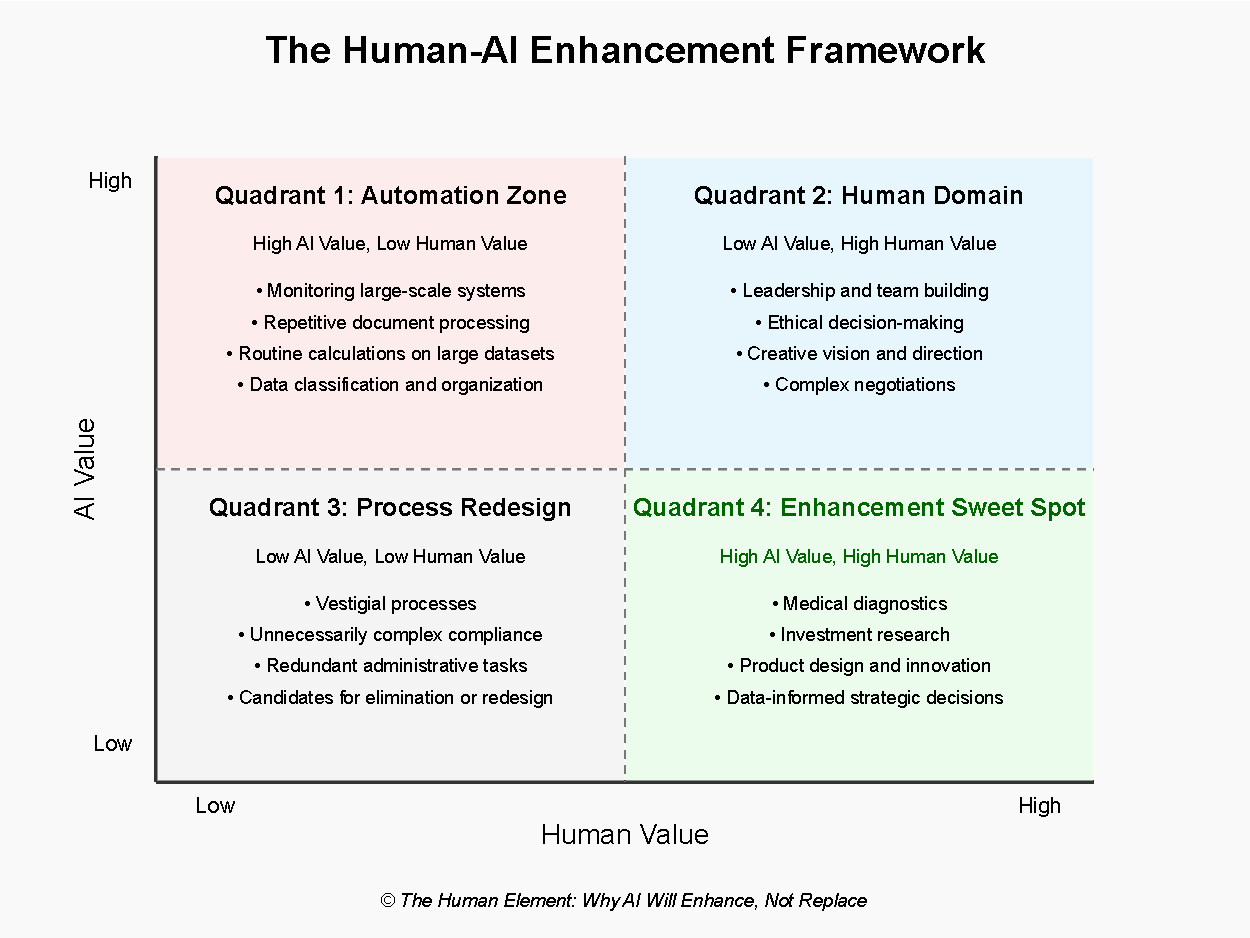
\includegraphics[width=0.8\textwidth]{_resources/images/CH06-images/enhancement-framework.pdf}

}

\caption{\label{fig-enhancement-framework}}

\end{figure}%

\textbf{Quadrant 1: High AI Value, Low Human Value}\\
These are tasks where AI consistently outperforms humans, and human
involvement adds little value. Examples include monitoring large-scale
systems for anomalies, repetitive document processing, and routine
calculations across large datasets. These activities are candidates for
automation\index{AI concepts!automation} rather than enhancement.

\textbf{Quadrant 2: Low AI Value, High Human Value}\\
These activities depend on qualities AI fundamentally lacks: empathy,
ethical judgment, creative vision, or contextual understanding that
transcends available data. Leadership, trust-building, innovative
ideation, and complex negotiations fall here. These should remain
primarily human domains.

\textbf{Quadrant 3: Low AI Value, Low Human Value}\\
These tasks benefit neither from human nor AI capabilities alone. They
typically represent vestigial processes that could be eliminated
entirely or fundamentally redesigned. Many regulatory compliance
activities and administrative processes fall into this category.

\textbf{Quadrant 4: High AI Value, High Human Value}\\
This is the enhancement sweet spot. Both AI and humans bring valuable
and complementary capabilities to these tasks. Medical diagnostics,
investment research, product design, and strategic
decision-making\index{AI concepts!decision-making} with significant data
components all reside here. These activities benefit most from
thoughtful human-AI
collaboration\index{human-AI relationship!human-AI collaboration}.

Organizations should systematically inventory their processes and map
them to these quadrants, prioritizing enhancement initiatives in
Quadrant 4 while pursuing automation in Quadrant 1 and process redesign
in Quadrant 3.

\section{Real-World Enhancement Sweet
Spots}\label{real-world-enhancement-sweet-spots}

Let's examine how leading organizations across industries have
identified and developed their enhancement sweet spots.

\textbf{Healthcare: Augmented Diagnostics}

Contrary to early predictions that AI would replace radiologists, the
most successful implementations enhance radiologists' capabilities
rather than attempting to substitute for them. Mayo
Clinic\index{case studies!Mayo Clinic}'s work with AI diagnostic tools
demonstrates this approach.

Their AI systems process medical images to identify potential
abnormalities, ranking findings by confidence level rather than making
binary judgments. Radiologists then apply their clinical expertise to
these machine-flagged areas, bringing contextual understanding of the
patient's history and presentation that the AI lacks.

This collaborative approach improves diagnostic accuracy while reducing
radiologist fatigue from screening thousands of normal images. It allows
radiologists to focus their specialized expertise where it adds most
value---on ambiguous cases and integrating findings with broader
clinical contexts.

Importantly, Mayo didn't simply deploy AI and expect radiologists to
adapt. They carefully redesigned workflows to optimize the human-AI
partnership, creating intuitive interfaces that present AI findings
without overwhelming human users with unnecessary technical details.

\textbf{Financial Services\index{financial services}: Enhanced Risk
Assessment}

JPMorgan\index{case studies!JPMorgan}'s implementation of Contract
Intelligence (COiN) shows how AI can enhance rather than replace human
judgment in financial services. The system reviews legal documents in
seconds rather than the 360,000 hours it would take humans, extracting
key provisions and flagging potential issues.

But final decisions still rest with experienced bankers who understand
client relationships, market contexts, and strategic priorities. The AI
handles the computational complexity of processing thousands of
documents, while humans provide judgment about how to respond to the
extracted information.

This enhancement approach delivers substantially greater value than
either automation or traditional manual processes alone. It reduces
costs and processing time while improving accuracy and consistency.
Perhaps most importantly, it redirects highly-compensated professionals
from low-value document review to high-value client service and
strategic thinking\index{human-AI relationship!strategic thinking}.

\textbf{Manufacturing and Transportation\index{transportation}: Enhanced
Human Capabilities}

BMW's implementation of AI in manufacturing quality control demonstrates
another successful enhancement approach. Their AI systems analyze images
from cameras positioned throughout the production line, identifying
potential defects with greater consistency than human inspectors could
achieve alone.

Rather than replacing quality inspectors, the system flags potential
issues for human review. Experienced inspectors bring contextual
understanding about which deviations matter and which don't---knowledge
that would be difficult to fully encode in an AI system.

This collaborative approach has reduced defect rates while allowing
human inspectors to focus on complex quality issues rather than routine
visual scanning. It combines AI's consistency and tirelessness with
human judgment about what constitutes acceptable quality in different
contexts.

A similar philosophy guides Daimler Trucks' approach to AI. Rather than
pursuing full autonomy at all costs, they developed AI systems that help
human drivers operate more safely and efficiently. The AI handles tasks
like maintaining safe following distances and optimizing fuel
consumption, while humans manage complex navigation and unexpected
situations. This stands in stark contrast to some autonomous vehicle
companies that have struggled by trying to eliminate human drivers
entirely.

\textbf{Creative Industries\index{creative industries}: Collaborative
Design}

While early AI art generators prompted fears about machines replacing
creative professionals, the enhancement approach is proving more
valuable. Design firm IDEO's work with generative
AI\index{AI concepts!generative AI} tools shows how this plays out in
practice.

Their designers use AI systems to rapidly generate design variations
based on initial parameters\index{AI concepts!parameters}. The AI
handles the computational aspects of design exploration, producing
dozens of options that would take humans significantly longer to create
manually.

Human designers then apply their aesthetic judgment, client
understanding, and cultural context to select, modify, and refine these
machine-generated options. The result combines AI's ability to explore a
wide design space with human designers' judgment about which options
meet client needs and resonate with target audiences.

Adobe\index{case studies!Adobe} has taken a similar approach with their
AI features. Rather than replacing designers, their tools handle tedious
tasks like image resizing and background removal, freeing humans to
focus on creative direction and client needs. Attempts to fully automate
creative work often disappoint, while approaches that enhance human
creativity succeed.

This enhancement approach accelerates the design process while
maintaining the essential human judgment that clients value. It allows
designers to explore more options in less time without sacrificing the
creative direction that distinguishes professional design from mere
iteration.

\section{Implementation Principles for Finding Your Sweet
Spot}\label{implementation-principles-for-finding-your-sweet-spot}

Organizations that successfully enhance human capabilities with AI
follow several key principles:

\textbf{The Role of Management and Cultural Considerations}

Finding the sweet spot requires rethinking traditional management
approaches. Leaders must understand both AI's capabilities and human
psychology. When McKinsey implemented AI tools for its consultants,
success came not from the technology itself but from careful attention
to how consultants would interact with it. The firm recognized that
consultants needed to maintain ownership of client relationships and
strategic insights while leveraging AI for research and analysis.

This highlights a crucial point: the enhancement sweet spot isn't
static. As AI capabilities evolve, the boundary between human and
machine tasks shifts. Organizations need adaptive frameworks that allow
for continuous rebalancing of responsibilities.

Perhaps most importantly, organizations must maintain ``human
centrality\index{human-AI relationship!human centrality}'' -- the
principle that AI serves human objectives rather than the reverse. This
requires careful attention to organizational
culture\index{implementation!organizational culture}. When Microsoft
deployed AI tools across its engineering teams, success came from
emphasizing how the technology would enhance rather than replace human
capabilities.

\textbf{Start with Human Needs, Not AI Capabilities}

Many AI implementations fail because they begin with the technology
rather than the problem. Organizations acquire AI solutions looking for
applications, rather than identifying specific human capabilities they
want to enhance.

Successful implementers reverse this approach. They start by asking:
``What human capabilities would we most like to enhance?'' This
human-centered perspective leads to more valuable applications than a
technology-driven implementation.

See for example how Stitch Fix approached AI implementation. Rather than
simply automating their stylists out of existence, they identified
specific aspects of the styling process where humans struggled with
computational complexity---managing thousands of inventory items across
multiple dimensions like size, color, style, and fabric. They then
developed AI tools that handled this complexity while preserving human
judgment about what would delight each specific customer.

This approach enhanced the capabilities of their human stylists rather
than replacing them. The result was more personalized recommendations
than either humans or algorithms could achieve alone.

\textbf{Design for Appropriate Division of Labor}

The interface between human and AI should leverage the strengths of
each. AI can process vast datasets and identify patterns, while humans
excel at contextual understanding and judgment. Design interactions that
optimize this complementarity.

Goldman Sachs\index{case studies!Goldman Sachs}' implementation of AI in
investment research exemplifies this principle. Their systems analyze
earnings transcripts, news reports, and market data at scales no human
analyst could match. But rather than generating automated investment
recommendations, the systems identify patterns and anomalies for human
analysts to investigate.

This division of labor plays to the strengths of each: AI handles data
processing at scale, while human analysts contribute contextual
understanding about market psychology, regulatory environments, and
competitive dynamics that may not be fully captured in the data.

\textbf{Build Trust Through Appropriate
Transparency\index{implementation!transparency}}

Users need appropriate visibility into how AI systems reach their
conclusions. The degree of transparency should match the stakes of the
decisions being supported---higher-stakes applications require greater
transparency and explainability.

Microsoft's implementation of AI-powered features in their development
tools illustrates this principle. When their Copilot system suggests
code, it provides context about where similar patterns have been used
before and the reasoning behind its suggestions. This transparency helps
developers maintain appropriate skepticism about AI recommendations
while leveraging its capabilities.

By contrast, some early medical AI systems operated as ``black boxes,''
providing diagnoses without explanation. This approach undermined
physician trust and limited adoption, regardless of technical accuracy.
Newer systems provide visualization of the patterns they've identified
and the reasoning behind their assessments, enabling appropriate human
oversight.

\textbf{Evolve Through Iteration}

The enhancement sweet spot shifts as both AI capabilities and human
practices evolve. Successful implementations establish feedback
mechanisms to continuously refine the human-AI partnership based on
real-world performance.

Netflix's recommendation system exemplifies this principle. Rather than
deploying a static algorithm, they continuously evaluate how users
interact with recommendations and refine their approach. This iterative
process has led to increasingly nuanced collaboration between
algorithmic recommendations and human content creators.

Similarly, Google\index{case studies!Google}'s implementation of AI in
search has evolved through continuous refinement based on user
interactions. The current system represents years of iterative
development to find the optimal balance between algorithmic processing
and human oversight.

\section{Finding Your Organization's Sweet
Spot}\label{finding-your-organizations-sweet-spot}

How can you identify and develop enhancement opportunities in your own
organization? We recommend a systematic approach:

\textbf{1. Process Inventory and Mapping}

Begin by inventorying key processes across your organization. For each
process, evaluate:

\begin{itemize}
\item
  Current performance metrics and pain points
\item
  The nature of human contribution (judgment, creativity, empathy, etc.)
\item
  Data availability and quality
\item
  Potential value of enhancement
\end{itemize}

Map these processes to the four-quadrant model described earlier,
prioritizing those in the high AI value/high human value quadrant for
enhancement initiatives.

Successful implementations require several key elements:

\begin{enumerate}
\def\labelenumi{\arabic{enumi}.}
\item
  \textbf{Clear role definition}: Both humans and AI need well-defined
  responsibilities that play to their strengths. At Goldman Sachs, AI
  handles data analysis and pattern recognition in trading, while human
  traders focus on strategy and risk assessment.
\item
  \textbf{Feedback loops\index{implementation!feedback loops}}: Humans
  must be able to override and correct AI when necessary. This isn't
  just about catching errors -- it's about maintaining human
  agency\index{human-AI relationship!human agency} and improving the
  system over time.
\item
  \textbf{Training and adaptation}: Workers need support in developing
  new skills that complement AI capabilities. The goal isn't to compete
  with AI but to leverage it effectively.
\end{enumerate}

\textbf{2. Pilot Selection and Design}

Select 1-3 high-potential processes for initial enhancement pilots. For
each pilot:

\begin{itemize}
\item
  Define clear success metrics that capture both efficiency and
  effectiveness
\item
  Design for appropriate division of labor between human and AI
\item
  Establish feedback mechanisms to capture user experience and
  suggestions
\item
  Plan for iteration based on early results
\end{itemize}

Resist the temptation to tackle too many processes simultaneously.
Enhancement requires careful design of the human-AI interaction, which
benefits from focused attention and learning from early implementations.

\textbf{3. Capability Building}

Successful enhancement requires new capabilities across the
organization:

\begin{itemize}
\item
  Technical teams need skills in human-centered design, not just AI
  development
\item
  Domain experts need understanding of AI capabilities and limitations
\item
  Leadership needs frameworks for evaluating enhancement opportunities
\item
  Everyone needs appropriate mental models for human-AI collaboration
\end{itemize}

Invest in building these capabilities alongside technical
implementation. Organizations that treat enhancement as purely a
technical challenge typically achieve lower returns than those that
invest in broader organizational capability building.

\textbf{4. Scaling and Evolution}

As pilots demonstrate value, develop plans for scaling successful
approaches while continuing to refine the human-AI interaction:

\begin{itemize}
\item
  Establish governance mechanisms to ensure consistent implementation
  while allowing for domain-specific adaptation
\item
  Build feedback loops to capture learning and identify improvement
  opportunities
\item
  Monitor for unintended consequences and adaptation needs
\item
  Continuously reassess the optimal division of labor as capabilities
  evolve
\end{itemize}

\section{Beyond Optimization: The Strategic Implications of
Enhancement}\label{beyond-optimization-the-strategic-implications-of-enhancement}

Finding your enhancement sweet spot delivers operational benefits
through improved efficiency and effectiveness. But the strategic
implications go further. Organizations that successfully enhance human
capabilities with AI gain several sustainable advantages:

\textbf{Talent Attraction and Retention}

As AI automates routine tasks, knowledge workers increasingly seek roles
that emphasize uniquely human capabilities like creativity, judgment,
and empathy. Organizations that design for enhancement rather than
replacement create more attractive roles that leverage these
capabilities.

The Mayo Clinic's approach to AI in radiology has made them more
attractive to top talent, not less. By enhancing radiologists'
capabilities rather than attempting to replace them, they've created
roles that emphasize the aspects of the profession that attracted
physicians to the field in the first place---using clinical judgment to
improve patient outcomes.

\textbf{Sustainable Competitive
Advantage\index{economic!competitive advantage}}

Enhancement approaches often create advantages that are harder for
competitors to replicate than pure automation. While algorithms can be
copied, the integration of AI capabilities with organization-specific
human expertise creates unique combinations that are difficult to
imitate.

JPMorgan's Contract Intelligence system delivers value not just through
its technical capabilities, but through its integration with the firm's
specific workflows, domain expertise, and client relationships. This
integrated approach creates a more sustainable advantage than either
technical capabilities or human expertise alone.

\textbf{System Resilience}

Enhancement approaches typically create more resilient systems than pure
automation. By maintaining appropriate human oversight and judgment,
these systems can better handle edge cases, adapt to changing
conditions, and recover from failures.

During the COVID-19 pandemic, organizations that had pursued enhancement
rather than replacement generally adapted more successfully to
unprecedented conditions. Their human-AI systems could incorporate new
information and adapt to changing circumstances more effectively than
fully automated approaches.

\textbf{Looking Forward: The Human-Centered Future of AI}

As AI capabilities continue to advance, finding the enhancement sweet
spot becomes increasingly crucial. Organizations that succeed will be
those that maintain focus on human judgment while leveraging AI's
computational power. This isn't just about efficiency -- it's about
creating sustainable competitive advantage through superior
decision-making.

Recall the evolution of chess after Deep Blue defeated Garry Kasparov.
Rather than eliminating human players, AI led to the emergence of
centaur chess, where human-AI teams consistently outperform either
humans or AI alone. This model points to the future of knowledge work:
not a competition between human and artificial
intelligence\index{AI concepts!artificial intelligence}, but a synthesis
that enhances human capabilities while preserving human agency.

The most valuable AI implementations of the coming decade will neither
attempt to replicate human capabilities nor eliminate human roles.
Instead, they will enhance human judgment, creativity, and
decision-making by handling computational complexity while preserving
space for uniquely human contributions.

Finding your enhancement sweet spot requires systematic evaluation of
where human and artificial intelligence can most effectively complement
each other. By applying the frameworks and principles outlined in this
chapter, organizations can move beyond simplistic automation narratives
toward more sophisticated enhancement strategies that create sustainable
value.

As Heidegger\index{philosophy!Heidegger} might suggest, the essence of
technology is nothing technological. The true value of AI lies not in
its technical capabilities alone, but in how those capabilities enhance
human potential. Organizations that understand this fundamental truth
will lead the next wave of innovation---not by developing the most
advanced AI systems, but by most effectively integrating AI with human
capabilities.

We expect to see continued evolution in how humans and AI interact. The
enhancement sweet spot will shift as AI capabilities advance, but the
fundamental principle remains: successful implementation requires
keeping humans central to decision-making while leveraging AI's unique
capabilities.

We return to our Cleveland Clinic cardiologist, who summarized it
perfectly: ``The AI doesn't replace my judgment---it extends my
capabilities. I can see patterns I might have missed while still
applying the contextual understanding that comes from years of clinical
experience. Together, we're better than either of us alone.''

That's the enhancement sweet spot---and finding yours is the key to
successful AI implementation.

\bookmarksetup{startatroot}

\chapter{The Implementation
Challenge}\label{the-implementation-challenge}

Practical strategies for introducing AI while maintaining human agency

\hfill\break

The gap between artificial
intelligence\index{AI concepts!artificial intelligence}'s theoretical
potential and its practical implementation remains stubbornly wide. Most
organizations approach AI implementation backward, starting with the
technology rather than the human element. They ask ``What can AI do?''
instead of ``How can we enhance our people's capabilities?'' This
fundamental mistake leads to costly failures and missed opportunities.

Recall the Fortune 500 consumer products company we mentioned in Chapter
6. Their project team, tasked with finding AI-driven productivity gains
from Microsoft\index{case studies!Microsoft}'s CoPilot suite, discovered
that while the technology could indeed compose email replies and
summarize meetings, users spent as much time editing the AI's output as
they would have spent writing from scratch. The AI was attempting to
replace rather than enhance human
capabilities\index{human-AI relationship!human capabilities}.

This pattern repeats across industries. Companies implement AI solutions
looking for quick automation\index{AI concepts!automation} wins, only to
discover that the technology works best when designed to augment human
judgment\index{human-AI relationship!human judgment} rather than replace
it. The key to successful implementation lies in understanding the
distinct roles of human and artificial intelligence, then building
systems that leverage the strengths of both.

\section{\texorpdfstring{The
Enhancement\index{human-AI relationship!enhancement} Framework in
Practice}{The Enhancement Framework in Practice}}\label{the-enhancement-framework-in-practice}

As we explored in Chapter 3, a clear framework for distinguishing
between tasks suitable for automation versus those that require human
enhancement is essential. This distinction often maps to what we have
described as the ``what versus how'' paradigm.

AI excels at executing the ``how'' - processing vast amounts of data,
identifying patterns, and generating outputs based on learned patterns.
Humans excel at determining ``what'' needs to be done, providing
context, and exercising judgment about the appropriateness of
AI-generated outputs. This framework helps organizations avoid the
common pitfall of trying to automate judgment-heavy tasks better suited
for enhancement.

In financial services\index{financial services}, AI can process market
data and generate trading signals at superhuman speed (the ``how''), but
successful firms keep humans in charge of setting strategy and risk
parameters\index{AI concepts!parameters} (the ``what'').
JPMorgan\index{case studies!JPMorgan}`s implementation of AI in its
trading operations demonstrates this principle. Rather than attempting
to fully automate trading decisions, the bank uses AI to enhance
traders' capabilities by surfacing relevant patterns and anomalies while
leaving final decisions to human judgment.

\section{\texorpdfstring{Building Trust Through
Transparency\index{implementation!transparency}}{Building Trust Through Transparency}}\label{building-trust-through-transparency}

One of the biggest implementation challenges is building trust between
human users and AI systems. This requires making the AI's capabilities
and limitations transparent to users while establishing clear boundaries
for human oversight.

The healthcare\index{healthcare} sector offers instructive examples.
Successful implementations of AI in medical
diagnosis\index{medical diagnosis} follow a clear pattern: the AI
processes medical images or patient data to flag potential issues (the
``how''), but doctors remain responsible for diagnosis and treatment
decisions (the ``what''). This approach maintains the critical element
of human judgment while leveraging AI's pattern-recognition
capabilities.

Crucially, these systems make their reasoning process visible to
doctors. Rather than simply presenting conclusions, they highlight the
specific patterns or anomalies that led to their recommendations. This
transparency helps build trust and enables doctors to exercise informed
judgment about the AI's suggestions.

Mayo Clinic\index{case studies!Mayo Clinic}'s deployment of AI tools in
radiology\index{radiology} exemplifies this approach. Their systems
don't simply classify images as ``normal'' or ``abnormal.'' Instead,
they highlight specific areas of potential concern and explain the
features that triggered the alert. This gives radiologists both valuable
information and critical context, allowing them to exercise professional
judgment informed by the AI's analysis.

\section{The Training Challenge: Beyond Technical
Skills}\label{the-training-challenge-beyond-technical-skills}

Implementing AI successfully requires significant investment in human
training, but not in the way most organizations expect. Rather than
focusing solely on technical training about how to use AI tools,
successful implementations emphasize training in judgment - helping
humans understand when and how to rely on AI assistance.

AeroVironment's implementation of AI in military applications is a
telling case. Operators receive extensive training not just in operating
the AI systems but in understanding their limitations and failure modes.
This approach produces operators who can effectively collaborate with AI
while maintaining the critical human judgment needed for military
operations.

The most effective training programs go beyond button-pushing
instructions to develop a proficiency akin to ``AI
literacy\index{implementation!AI literacy}'' - a sophisticated
understanding of what AI does well, where it struggles, and how to
evaluate its outputs critically. This requires a combination of
technical knowledge and domain expertise.

Goldman Sachs\index{case studies!Goldman Sachs} takes this approach with
their AI-enhanced investment tools. Analysts learn not just how to use
the tools but how to identify situations where the AI's recommendations
might be biased by historical patterns that no longer apply or where
additional human judgment is crucial. This balanced approach maintains
the human element while leveraging AI's computational strengths.

\section{Measuring Success Beyond
Efficiency}\label{measuring-success-beyond-efficiency}

Traditional metrics often fail to capture the true value of AI
enhancement implementations. Organizations frequently focus on easily
measurable efficiency gains while missing the more substantial benefits
of enhanced human judgment and
decision-making\index{AI concepts!decision-making}. This approach gives
too much weight to all the things that can be measured, and not enough
attention to those that cannot be.

Palantir\index{case studies!Palantir}'s implementations offer a model
for better measurement. Rather than focusing solely on automation
metrics, they measure success through the quality of human-AI
collaboration\index{human-AI relationship!human-AI collaboration} -
tracking how effectively analysts use AI tools to reach better
conclusions faster. This approach recognizes that AI's value lies not in
replacing human analysts but in enhancing their capabilities.

Effective measurement frameworks consider both quantitative improvements
(time saved, volume processed) and qualitative outcomes (decision
quality, novel insights generated, unexpected connections identified).
The latter often represent the true value of enhancement approaches but
require more sophisticated measurement approaches.

A major healthcare system found that its AI-assisted diagnostic system
reduced the time radiologists spent reviewing normal scans by 31\%, a
clear efficiency gain. But the more valuable outcome was a 22\% increase
in early detection of subtle abnormalities that might otherwise have
been missed. This qualitative improvement in diagnostic accuracy
represented the true value of the system, though it was harder to
measure than simple time savings.

\section{Common Implementation
Pitfalls}\label{common-implementation-pitfalls}

Several common mistakes consistently undermine AI implementation
efforts. First among these is overemphasis on automation. Organizations
often focus on fully automating processes rather than enhancing human
capabilities. This leads to resistance from users and missed
opportunities for genuine enhancement.

Another frequent error is insufficient training in judgment. Most
training programs focus on technical operation rather than helping users
understand when and how to rely on AI assistance. This leads to either
over-reliance on AI recommendations or underutilization of AI
capabilities.

Poor integration with existing workflows represents another significant
challenge. AI tools are often implemented as standalone solutions rather
than being integrated into existing work processes. This creates
friction for users and reduces adoption and effectiveness.

Many implementations also suffer from a lack of clear boundaries
regarding which decisions require human judgment and which can be
delegated to AI. Without these guidelines, organizations often drift
toward excessive automation, undermining human judgment and creating
potential risks.

Finally, inadequate feedback loops\index{implementation!feedback loops}
plague many AI implementations. Without effective mechanisms for humans
to provide feedback on AI performance and for that feedback to improve
the system, AI systems fail to improve over time and users lose
confidence in their reliability.

\section{The Path to Successful
Implementation}\label{the-path-to-successful-implementation}

Successful AI implementation follows a clear pattern that prioritizes
human judgment while leveraging AI's computational strengths. The
process starts with identifying where human judgment adds the most value
in your organization. These areas are typically candidates for
enhancement rather than automation.

McKinsey's implementation of AI tools for their consulting practice
demonstrates this approach. They first mapped how their best consultants
synthesized information and formulated recommendations. This revealed
that while data analysis could be enhanced by AI, the crucial skills of
problem framing and solution crafting relied heavily on human judgment
and client relationship understanding.

Designing for transparency represents another critical element. AI
systems should make their reasoning visible to users, enabling informed
human oversight. This goes beyond simple explanations of AI decisions.
The system should reveal its confidence levels, data sources, and key
factors influencing its recommendations. Users should be able to trace
the logic chain from input to output.

Microsoft's implementation of AI coding assistants demonstrates this
principle. Rather than simply generating code, the system highlights the
patterns and documentation it references, allowing developers to
understand and validate its suggestions. This transparency helps
developers maintain control while benefiting from AI assistance.

Gradual integration provides another key to success. Beginning with
small-scale implementations allows users to build trust and
understanding of the AI's capabilities and limitations. This approach
creates opportunities for learning and adjustment without risking major
disruption.

Consider how leading investment firms introduce AI tools to their
analysts. They typically begin with using AI for initial data screening
and pattern detection, allowing analysts to compare AI insights with
their traditional methods. As confidence builds, they gradually expand
the AI's role while maintaining human oversight of investment decisions.

Establishing clear boundaries defines explicit guidelines for which
decisions require human judgment and which can be delegated to AI. These
boundaries should be based on careful analysis of risk, regulatory
requirements, and the comparative advantages of human and artificial
intelligence.

JPMorgan's AI implementation in trading provides an instructive example.
They maintain clear rules about which types of trades can be executed
automatically versus which require human review. These boundaries
consider factors like transaction size, market conditions, and potential
impact on other positions. The rules are regularly reviewed and updated
based on performance data and changing market conditions.

Building effective feedback loops creates mechanisms for continuous
improvement based on human feedback about AI performance. This requires
more than simple error reporting. Users should be able to provide
context about why certain AI recommendations were helpful or unhelpful,
identify emerging edge cases, and suggest improvements to the system's
operation.

Palantir's implementations demonstrate the power of well-designed
feedback loops. Their systems allow analysts to flag both false
positives and false negatives, provide context about why certain
connections are meaningful or meaningless, and suggest new patterns for
the system to consider. This feedback is systematically reviewed and
incorporated into system improvements.

\section{Cultural Change Management}\label{cultural-change-management}

The human element in AI implementation extends beyond technical
considerations to encompass cultural factors. Organizations must help
employees understand that AI tools are meant to enhance their
capabilities, not replace them. This often requires active effort to
counter fears and misconceptions about AI.

When Starbucks\index{case studies!Starbucks} implemented AI tools for
inventory management and scheduling, they emphasized how the technology
would free baristas from administrative tasks to focus on customer
interaction and craft beverages. This positive framing helped overcome
initial resistance and accelerated adoption.

Continuous training supports this cultural shift. As AI capabilities
evolve, users need ongoing training to make effective use of new
features and capabilities. This training should focus on judgment and
decision-making rather than just technical operation. Organizations that
invest in this ongoing development typically see higher returns on their
AI investments.

Regular review and adjustment complete the implementation cycle.
Periodically reviewing the implementation's effectiveness against its
goals reveals areas where the balance between automation and enhancement
needs adjustment. This iterative approach recognizes that finding the
optimal human-AI collaboration requires continuous refinement.

\section{Looking Ahead: The Future of
Implementation}\label{looking-ahead-the-future-of-implementation}

As AI capabilities continue to advance, the implementation challenge
will evolve. Vector databases\index{AI concepts!vector databases}, for
example, are emerging as a crucial tool for enhancing human search and
discovery capabilities. These systems don't replace human judgment but
rather augment it by making conceptual connections that might otherwise
be missed.

However, the fundamental principle remains: successful implementation
requires keeping humans central to the process. As one senior technology
executive noted, ``The goal isn't to make the AI smarter, but to make
the human-AI collaboration more effective.''

This principle extends beyond mere oversight; it recognizes that human
judgment, intuition, and accountability are essential elements of
effective decision-making. The most successful AI implementations
maintain what critics have called ``seeing the human doing it'' - the
visible presence of human judgment and accountability in key decisions.

Think of the creative industries\index{creative industries}, where AI
tools are increasingly common but rarely trusted to work autonomously.
The attempt to use AI to complete Beethoven\index{Beethoven}'s
unfinished tenth symphony, which we discussed in detail in Chapter 8,
demonstrates this principle. While the AI could generate music that
superficially resembled Beethoven's style, critics and audiences alike
found it lacking the essential human element that makes great art
compelling.

\section{Investment Implications}\label{investment-implications-3}

For investors and business leaders, understanding these implementation
challenges is crucial. Success in AI implementation often correlates
more strongly with an organization's ability to enhance human
capabilities than with the sophistication of its AI technology.

Companies that demonstrate a sophisticated understanding of human-AI
collaboration, with clear frameworks for maintaining human judgment
while leveraging AI capabilities, are more likely to succeed in the long
term. This insight should guide both investment decisions and
implementation strategies.

When evaluating AI investments, look beyond technical capabilities to
assess how effectively the company addresses the human element in
implementation. Does the company have a clear enhancement
framework\index{implementation!enhancement framework}? Do they emphasize
transparency and explainability? Have they developed effective training
approaches for users? Do they have mechanisms for continuous improvement
based on human feedback?

The most promising investments often come not from companies pursuing
the most advanced AI capabilities but from those that most effectively
integrate AI with human judgment and expertise. This enhancement-focused
approach typically delivers more sustainable value than pure automation
plays.

\section{Conclusion}\label{conclusion}

Successful AI implementation requires a fundamental shift in thinking -
from automation to enhancement, from replacement to
augmentation\index{human-AI relationship!augmentation}. Organizations
that master this shift, keeping humans central while leveraging AI's
capabilities, will be best positioned to create sustainable value in the
AI era.

The challenge isn't primarily technical - it's organizational and human.
Success requires careful attention to human factors, clear frameworks
for collaboration, and a commitment to enhancing rather than replacing
human capabilities. As AI continues to evolve, this human-centric
approach to implementation will become increasingly crucial for
organizational success.

By following the implementation principles outlined in this chapter -
starting with human judgment, designing for transparency, integrating
gradually, establishing clear boundaries, and building feedback loops -
organizations can avoid the common pitfalls that plague many AI
initiatives and instead develop systems that truly enhance human
capabilities.

The future belongs not to organizations that deploy the most
sophisticated AI systems but to those that most effectively combine
artificial and human intelligence, creating systems that are more
powerful than either could be alone. This is the true promise of AI
enhancement - and the key to successful implementation.

\bookmarksetup{startatroot}

\chapter{The Human Exception in Creative
Work}\label{the-human-exception-in-creative-work}

Lessons from Beethoven's Tenth: Why `seeing the human doing it' remains
crucial across industries

\hfill\break

We now have mentioned the Beethoven\index{Beethoven} experiment several
times because it is at the center of the theme in this book. An all-star
team of musicologists, historians, and AI programmers attempted
something unprecedented: completing Beethoven's unfinished Tenth
Symphony using artificial
intelligence\index{AI concepts!artificial intelligence}. By the
reckoning of most experts, they ultimately failed to create a new
version of the great composer's work. From our perspective, this project
offers valuable insights into both the capabilities and limitations of
AI in creative work, while illuminating why human
authenticity\index{philosophy!authenticity} remains irreplaceable even
as AI capabilities advance.

\section{The Beethoven Challenge}\label{the-beethoven-challenge}

Beethoven left the world with nine completed symphonies and a handful of
musical sketches for a tenth. For centuries, these fragments tantalized
musicians and scholars, hinting at what might have been. The AI team at
Playform AI saw an opportunity: they would train their models on
Beethoven's complete works, use the sketches as a foundation, and
generate what they believed would be a plausible completion of the Tenth
Symphony.

On paper, this appeared to be an ideal AI project. The team had:

\begin{itemize}
\tightlist
\item
  A complete corpus of Beethoven's work for training
\item
  Actual sketches from the composer for the specific piece
\item
  Access to leading experts in both music and AI
\item
  State-of-the-art machine learning\index{AI concepts!machine learning}
  capabilities
\end{itemize}

If AI could successfully complete this task, it would demonstrate
remarkable creative capabilities. The result would be more than just a
technical achievement -- it would show that AI could authentically
channel human genius.

\section{The Results: Technical Success, Artistic
Failure}\label{the-results-technical-success-artistic-failure}

The resulting symphony is technically impressive. To an untrained ear,
it sounds plausibly like classical music. The notes follow reasonable
progressions, the orchestration is proper, and there are moments that
sound distinctly Beethoven-esque. Yet something crucial is missing.

As Beethoven scholar Jan Swafford noted in his review, the work is
``aimless and uninspired.'' The missing element isn't technical
proficiency -- it's the human struggle for excellence, the creative
tension that produces true artistic breakthrough. This reveals a
fundamental truth about AI that extends far beyond music: technical
competence is not the same as authentic creation.

\section{The Role of Human Struggle}\label{the-role-of-human-struggle}

Swafford's critique points to something deeper about human creativity:
``We humans need to see the human doing it: Willie Mays making the catch
that doesn't look possible. When it comes to art, we need to see a woman
or a man struggling with the universal mediocrity that is the natural
lot of all of us and somehow out of some mélange of talent, skill, and
luck doing the impossible.''

This insight helps explain why even technically perfect AI creations
often feel hollow. Consider:

\begin{enumerate}
\def\labelenumi{\arabic{enumi}.}
\item
  \textbf{The Value of Imperfection}: Beethoven's own sketches were
  often mundane and uninspired. It was through sustained effort and
  refinement that he transformed ordinary musical ideas into
  extraordinary compositions. The process itself -- the human struggle
  -- is part of what we value.
\item
  \textbf{Quality Discrimination}: Training AI on all of Beethoven's
  works presents another challenge: Beethoven himself sometimes wrote
  mediocre pieces when working on commission. The AI cannot distinguish
  between his masterpieces and his mere commercial work. It lacks the
  human judgment\index{human-AI relationship!human judgment} to separate
  the transcendent from the ordinary.
\item
  \textbf{Emotional Connection}: The audience's knowledge that a human
  created the work is part of the work's meaning. We connect with art
  partly because we know another human being struggled to create it.
\end{enumerate}

\section{Beyond Music: The Broader
Implications}\label{beyond-music-the-broader-implications}

This principle -- that we need to ``see the human doing it'' -- extends
far beyond classical music. Here are some parallels:

\subsection{Sports and Entertainment}\label{sports-and-entertainment}

The same dynamic explains why robotic sports would never generate the
passion of human athletics. When Colombian and Argentine soccer fans
stormed Miami's Hard Rock Stadium to see Lionel Messi play, they weren't
just seeking to witness technical excellence -- they wanted to see human
brilliance in action. No matter how technically sophisticated, robots
playing soccer would never generate such emotional investment.

\subsection{Business Leadership}\label{business-leadership}

In corporate settings, technically correct decisions aren't always the
best decisions. Leaders need to be seen making difficult choices,
wrestling with uncertainty, and taking responsibility for outcomes. An
AI might make statistically optimal decisions, but it cannot provide the
human element that builds trust and inspires teams.

\subsection{Professional Services}\label{professional-services}

Even in fields where technical expertise is paramount -- law\index{law},
medicine, financial advice -- clients need to see human judgment at
work. They need to know that a human professional has wrestled with
their unique situation and exercised judgment on their behalf.

\section{\texorpdfstring{The
Enhancement\index{human-AI relationship!enhancement}
Opportunity}{The Enhancement Opportunity}}\label{the-enhancement-opportunity}

The Beethoven experiment reveals the true opportunity for AI in creative
fields: enhancement rather than replacement. AI can be an invaluable
tool for: - Generating initial ideas - Testing different approaches -
Handling technical aspects of implementation - Providing feedback and
suggestions

But the human element remains essential for: - Exercise of judgment -
Quality discrimination - Emotional resonance - Authentic creation

\section{Looking Forward}\label{looking-forward}

As AI capabilities continue to advance, maintaining this balance between
human authenticity and AI enhancement becomes crucial. Organizations
that understand this will: - Keep humans visibly involved in key
creative and decision-making\index{AI concepts!decision-making}
processes - Use AI to augment rather than replace human judgment -
Maintain transparency\index{implementation!transparency} about the role
of AI in their processes - Invest in developing human creativity and
judgment alongside AI capabilities

The lesson from Beethoven's Tenth is clear: technical proficiency, even
at a very high level, is not enough. The human
exception\index{human-AI relationship!human exception} -- the visible
struggle for excellence, the exercise of judgment, the emotional
connection -- remains irreplaceable. This insight should guide how we
implement AI across industries and applications.

Success in an AI-enhanced world doesn't mean replacing human creativity
and judgment with artificial intelligence. Instead, it means finding
ways to use AI that preserve and amplify the human elements that create
true value. The goal should be to let AI handle the technical ``how''
while humans focus on the essential ``what'' -- the judgment,
creativity, and authentic connection that only humans can provide.

\bookmarksetup{startatroot}

\chapter{Following the Money}\label{following-the-money}

Investment Implications of the Enhancement Thesis: Identifying winners
and losers in an AI-enhanced economy

\hfill\break

The investment implications of artificial
intelligence\index{AI concepts!artificial intelligence} extend far
beyond the obvious beneficiaries in Silicon Valley. While companies like
Nvidia have captured headlines with astronomical returns, the real
opportunity lies in identifying businesses that effectively leverage AI
to enhance rather than replace human
capabilities\index{human-AI relationship!human capabilities}. This
nuanced view requires looking past the hype to understand how AI
actually creates sustainable competitive advantages.

The distinction between ``what'' and ``how'' intelligence provides a
powerful framework for understanding investment opportunities in the AI
era. While much of the market's attention has focused on pure AI plays
and dramatic automation\index{AI concepts!automation} narratives, the
reality emerging from successful implementations suggests a more nuanced
landscape---one where value accrues to companies that effectively
leverage both domains rather than emphasizing one at the expense of the
other.

This framework moves beyond simplistic replacement narratives to
identify where sustainable competitive advantages are likely to emerge.
As we've explored throughout this book, AI excels at executing the
``how''---implementing well-defined processes and handling computational
complexity---while humans maintain advantages in the
``what''---determining strategic direction, exercising judgment, and
framing problems effectively. The investment opportunities created by
this division extend far beyond the obvious technology players to
include companies across sectors that successfully integrate these
complementary capabilities.

\section{The What-How Investment
Landscape}\label{the-what-how-investment-landscape}

The investment landscape emerging from the what-how divide falls into
three primary categories, each with distinct value propositions and
competitive dynamics.

First, ``How Specialists'' create value by transforming implementation
capabilities across industries. These companies develop the
infrastructure and tools that enable AI to execute with unprecedented
efficiency and scale. The most obvious examples include semiconductor
manufacturers like Nvidia, whose specialized chips dramatically
accelerate AI computations, and cloud computing platforms that provide
the infrastructure for deploying AI at scale. But this category extends
beyond hardware to include companies developing specialized AI tools for
particular implementation domains---from code generation to image
processing to natural language production.

The competitive advantages in this category derive from scale economies,
network effects, and technical leadership. Nvidia's dominance, for
instance, extends beyond its hardware capabilities to encompass its CUDA
software ecosystem, which creates powerful switching costs for
developers. Similarly, cloud providers like
Microsoft\index{case studies!Microsoft} Azure and
Google\index{case studies!Google} Cloud build advantages through
integrated AI services that simplify implementation for enterprise
customers.

Second, ``What Enablers'' focus on enhancing human strategic
decision-making\index{AI concepts!decision-making} rather than replacing
it. These companies develop tools and platforms that augment human
judgment\index{human-AI relationship!human judgment} by processing vast
amounts of data, identifying patterns, and generating insights that
inform strategic decisions. Examples include companies like
Palantir\index{case studies!Palantir}, whose platforms help human
analysts make sense of complex data environments, and decision support
tools in healthcare\index{healthcare} that help doctors identify
potential diagnoses while preserving their clinical judgment.

Competitive advantages for What Enablers tend to be more
domain-specific, deriving from deep understanding of particular decision
contexts, accumulated data assets, and the ability to effectively
interface between AI capabilities and human judgment. The most
successful companies in this category don't merely provide raw
analytical capabilities; they package insights in ways that meaningfully
enhance human decision-making within specific contexts.

Third, ``Integration Masters\index{economic!integration masters}''
successfully bridge both domains, creating seamless connections between
human strategic direction and AI-powered implementation. These
companies---often enhanced incumbents rather than pure AI
plays---leverage artificial intelligence to amplify existing competitive
advantages rather than creating entirely new business models. They
maintain human judgment in areas where it adds most value while
deploying AI to handle implementation complexity at unprecedented scale
and consistency.

JPMorgan\index{case studies!JPMorgan} exemplifies this approach in
financial services\index{financial services}, using AI to process vast
amounts of transaction data and flag potential issues while maintaining
human judgment for complex risk assessments and client relationships.
Similarly, Mayo Clinic\index{case studies!Mayo Clinic} enhances
radiologist capabilities through AI that processes medical images while
preserving physician judgment for diagnosis and treatment decisions.

The most sustainable competitive advantages often emerge in this third
category, where companies create integrated capabilities that
competitors cannot easily replicate. While individual AI technologies
might be widely available, the effective integration of these
capabilities with domain-specific human expertise creates moats that
prove remarkably durable.

\section{\texorpdfstring{Value Creation\index{economic!value creation}
Through the What-How
Lens}{Value Creation Through the What-How Lens}}\label{value-creation-through-the-what-how-lens}

Companies that effectively navigate the what-how divide demonstrate
distinct performance advantages across several key metrics---creating
investment signals that savvy investors can leverage to identify future
winners.

First, productivity metrics\index{economic!productivity metrics} reveal
the efficiency gains from appropriate division of labor between humans
and AI. Rather than simply automating to reduce headcount, successful
implementations redirect human cognitive capacity toward higher-value
activities while leveraging AI for routine execution. This shows up in
metrics like revenue per employee, which typically increases 30-40\%
within 3-5 years of effective implementation---significantly outpacing
the 15-20\% improvements from pure automation approaches.

The way that Bloomberg\index{case studies!Bloomberg} has evolved its
financial terminal business is a case in point. Rather than simply
automating financial analysis, they've used AI to process vast amounts
of market data while keeping humans focused on identifying relevant
patterns and developing investment insights. The result is dramatically
higher productivity per analyst while maintaining the high-touch service
that justifies premium pricing.

Second, capital efficiency\index{economic!capital efficiency} improves
through more targeted technology investments. Companies that understand
the what-how
distinction\index{human-AI relationship!what-how distinction} tend to
make smaller, more focused AI investments with clearer payback periods
rather than massive infrastructure projects with uncertain returns. This
shows up in metrics like return on invested
capital\index{economic!return on invested capital} (ROIC), which
typically remains 800-1200 basis points above cost of capital for
companies pursuing balanced
enhancement\index{human-AI relationship!enhancement}
strategies---roughly double the premium for those focused solely on
automation.

Goldman Sachs\index{case studies!Goldman Sachs}' approach to AI
investment exemplifies this efficiency. Rather than attempting to
automate their entire investment process, they've made targeted
investments in specific capabilities---like natural language processing
for earnings calls and sentiment analysis for news events---while
maintaining human judgment for investment decisions. This focused
approach has delivered clearer returns than competitors pursuing more
sweeping AI transformations.

Third, customer relationships strengthen when companies enhance rather
than replace human elements in their service delivery. This manifests in
metrics like Net Promoter Score (NPS), customer retention rates, and
share of wallet---all of which tend to be significantly higher for
companies that maintain appropriate human involvement in customer-facing
roles while leveraging AI for background processes.

The contrast between different approaches to wealth management
automation illustrates this dynamic clearly. The first wave of
robo-advisors attempted to completely automate investment
management\index{investment management}, promising lower fees through
elimination of human advisors. While they achieved some success in basic
portfolio allocation, they struggled to retain high-net-worth clients
who value human judgment in complex financial planning. In contrast,
firms that deployed AI to enhance their human advisors'
capabilities---providing better analytics, freeing time for client
relationships, enabling more sophisticated planning---have seen superior
results across key relationship metrics.

Fourth, competitive advantages prove more sustainable when built on the
integration of AI capabilities with human expertise rather than
technology alone. While pure technology advantages typically erode as
innovations disseminate, the combination of AI implementation with
domain-specific human judgment creates integrated capabilities that
competitors struggle to replicate. This
sustainability\index{economic!sustainability} shows up in metrics like
gross margin stability and market share\index{economic!market share}
retention over time.

LVMH\index{case studies!LVMH}'s application of AI in luxury retail
demonstrates this sustainability. Rather than eliminating human sales
associates, they've deployed AI to enhance personalization capabilities
and inventory management while maintaining the high-touch human service
that luxury customers expect. The resulting combination has proven
remarkably difficult for competitors to match, allowing the company to
maintain premium pricing and market leadership even as technology
proliferates.

Finally, regulatory risk\index{economic!regulatory risk} decreases when
companies maintain appropriate human oversight and accountability. As
regulatory frameworks\index{policy!regulatory frameworks} for AI
continue to evolve, companies that preserve human judgment in critical
decisions face substantially lower compliance burdens and fewer
regulatory incidents than those pursuing full automation. This risk
differential shows up directly in compliance costs, which average
30-40\% lower for companies pursuing balanced human-AI strategies.

\section{The What-How Integration
Matrix}\label{the-what-how-integration-matrix}

To visualize these dynamics, we propose a framework called the
``What-How Integration Matrix'' that maps companies based on their
capabilities in both domains. This matrix helps investors identify where
particular organizations fall within the landscape and evaluate their
potential for sustainable value creation.

\pandocbounded{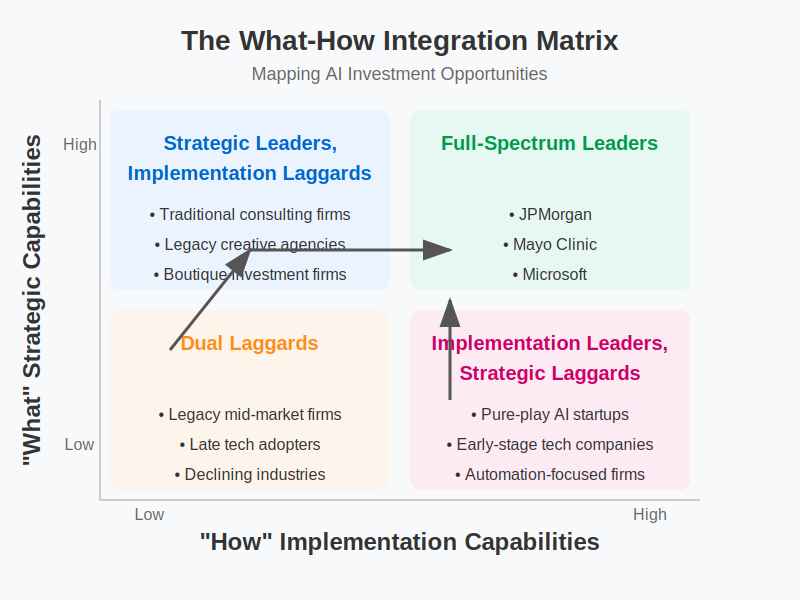
\includegraphics[keepaspectratio]{index_files/mediabag/_resources/images/Ch09-images/what-how-matrix-ch9.pdf}}

The vertical axis represents capabilities in the ``what'' domain---the
ability to frame problems effectively, exercise contextual judgment, and
set strategic direction. Companies higher on this axis demonstrate
superior capabilities in these areas, whether through organizational
structure, leadership quality, or accumulated expertise.

The horizontal axis represents capabilities in the ``how'' domain---the
ability to implement efficiently at scale through AI and related
technologies. Companies further to the right on this axis have more
sophisticated implementation capabilities, whether through technical
infrastructure, data assets, or algorithmic sophistication.

This creates four quadrants, each with distinct investment implications:

In the upper right quadrant are ``Full-Spectrum Leaders''---companies
with strong capabilities in both domains. These organizations
effectively leverage AI for implementation while maintaining strong
human judgment in strategic areas. Examples include JPMorgan in
financial services, Mayo Clinic in healthcare, and Microsoft in
enterprise software. These companies typically deliver superior
financial performance across multiple metrics and maintain sustainable
competitive advantages. They represent the most attractive long-term
investments in the AI landscape.

In the upper left quadrant are ``Strategic
Leaders\index{economic!strategic leaders}, Implementation
Laggards''---companies with strong strategic capabilities but
underdeveloped AI implementation. These organizations maintain valuable
human judgment but haven't yet leveraged AI effectively to execute at
scale. Examples include many traditional consulting firms and creative
agencies. These companies represent potential turnaround opportunities
if they can successfully develop implementation capabilities while
preserving their strategic strengths.

In the lower right quadrant are ``Implementation
Leaders\index{economic!implementation leaders}, Strategic
Laggards''---companies with sophisticated AI capabilities but
underdeveloped strategic judgment. These organizations execute
efficiently at scale but struggle with determining what's worth doing in
the first place. Examples include many pure-play AI startups and
early-stage technology companies. These companies often deliver
impressive technical results but struggle with sustainable business
models. They represent higher-risk investments that might deliver
breakthroughs but face significant strategic challenges.

In the lower left quadrant are ``Dual
Laggards\index{economic!dual laggards}''---companies with weak
capabilities in both domains. These organizations neither leverage AI
effectively nor maintain distinctive human judgment. They represent the
least attractive investment opportunities and face existential threats
as competition intensifies.

The most successful companies typically follow an upward trajectory
through this matrix over time, either by enhancing their ``what''
capabilities through organizational development or by improving their
``how'' capabilities through technological investment. Understanding
where companies fall on this matrix---and how they're
evolving---provides invaluable insight for investment decisions.

\section{Industry-Specific
Applications}\label{industry-specific-applications}

The what-how framework manifests differently across industries, creating
distinct investment opportunities in each sector.

In financial services, the divide appears most clearly between strategic
risk assessment and transaction execution. Companies like BlackRock have
leveraged this distinction effectively, using AI to handle routine
trading operations and data analysis while maintaining human judgment
for portfolio construction and risk management. Their Aladdin platform
exemplifies this approach, providing sophisticated analytical
capabilities while preserving human oversight for strategic decisions.
The result has been dramatic growth in assets under management while
maintaining impressive margins\index{economic!margins}.

The contrast with pure algorithmic trading firms is instructive. While
many quantitative hedge funds have delivered impressive short-term
results through AI-driven strategies, they've also demonstrated greater
volatility and vulnerability to market shifts that fall outside their
training data\index{AI concepts!training data}. The most sustainable
advantages have emerged not from pure automation but from firms that
effectively combine algorithmic execution with human judgment about
market conditions and risk factors.

In healthcare, the divide manifests between diagnostic judgment and data
processing. Companies like Tempus have built successful models by
enhancing physician capabilities rather than attempting to replace them.
Their platform analyzes vast amounts of clinical and molecular data to
identify potential treatment options while maintaining doctor judgment
for diagnosis and treatment selection. This approach has enabled them to
build a sustainable business model with strong hospital relationships
that pure automation plays have struggled to match.

The pharmaceutical industry demonstrates similar dynamics. Companies
like Recursion Pharmaceuticals use AI to dramatically accelerate drug
discovery processes that would be impossible for humans to execute
manually, while maintaining scientific judgment about which compounds
merit further investigation. This combination has enabled them to build
a more capital-efficient drug discovery model than either traditional
pharma companies or pure AI startups.

In manufacturing\index{manufacturing}, the divide appears between design
creativity and production optimization. Companies like NVIDIA have
mastered this distinction not just in their products but in their own
operations. They leverage AI extensively in chip design and production
processes while maintaining human creativity in architectural decisions
and strategic direction. This combination has enabled them to maintain
technical leadership while achieving unprecedented scale.

BMW's implementation of AI in manufacturing quality control demonstrates
similar principles. Their systems process visual inspection data at
scale and consistency impossible for humans, while maintaining human
judgment for determining which deviations matter in different contexts.
The result has been dramatic improvements in quality metrics while
maintaining the distinctive characteristics that define their brand.

In creative industries\index{creative industries}, the divide manifests
between artistic vision and technical execution. Companies like
Pixar\index{case studies!Pixar} exemplify this approach, using
increasingly sophisticated AI tools for rendering and animation while
preserving human creativity for storytelling and character development.
This combination has enabled them to create films of increasing
technical sophistication while maintaining the emotional resonance that
drives commercial success.

Adobe\index{case studies!Adobe} has followed a similar path with their
Creative Cloud suite, integrating increasingly powerful AI capabilities
while preserving space for human creative direction. Their Generative
Fill features, for instance, handle technical execution that would be
tedious for humans while keeping designers in control of creative
vision. This approach has enabled them to maintain premium pricing and
market leadership despite increasing competition.

\pandocbounded{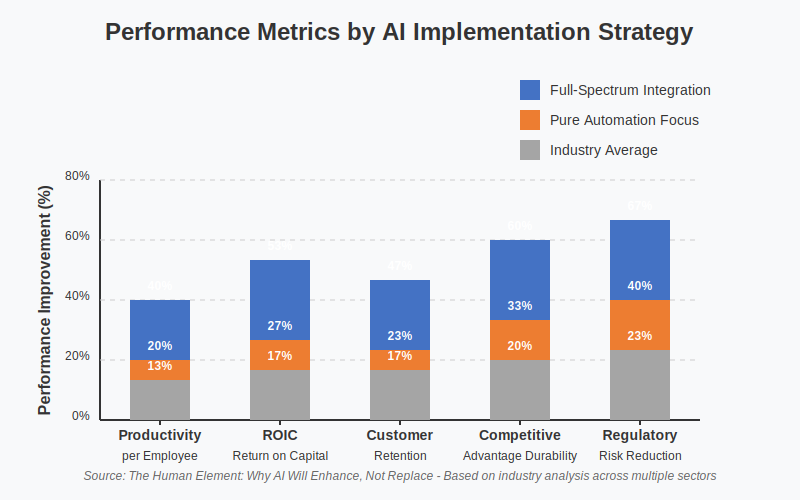
\includegraphics[keepaspectratio]{index_files/mediabag/_resources/images/Ch09-images/performance-chart.pdf}}

\section{\texorpdfstring{Investment
Strategy\index{economic!investment strategy}
Implications}{Investment Strategy Implications}}\label{investment-strategy-implications}

The what-how framework suggests several key principles for AI-related
investment strategies:

First, focus on integration capabilities rather than pure AI technology.
The most sustainable advantages emerge not from technical leadership in
isolation but from effective integration of AI capabilities with
domain-specific human expertise. Companies that demonstrate
sophisticated understanding of the appropriate boundaries between human
and AI responsibilities typically outperform pure technology plays over
the long term.

Second, evaluate leadership understanding of the what-how distinction.
Companies whose executives can clearly articulate where human judgment
adds value versus where AI can handle implementation typically
demonstrate superior implementation results. This understanding shows up
in organizational structure, talent development approaches, and capital
allocation decisions.

Third, assess data assets and implementation capabilities realistically.
While many companies tout their AI initiatives, the reality often falls
short of the rhetoric. Investors should look for concrete evidence of
implementation success---clear use cases, measurable results, and
realistic assessments of both capabilities and limitations.

Fourth, consider timing and geographic diversification. Different
industries and regions are at different stages of AI adoption, creating
opportunities to identify leaders in emerging domains before full market
recognition. This requires careful attention to adoption curves and
industry-specific implementation challenges.

Fifth, monitor regulatory developments through the what-how lens.
Regulatory frameworks increasingly distinguish between different levels
of automation and human oversight. Companies that maintain appropriate
human involvement in critical decisions typically face lower regulatory
burdens than those pursuing full automation strategies.

The most attractive investments typically demonstrate several
characteristics: clear understanding of where human judgment adds value,
sophisticated AI implementation in appropriate domains, strong data
assets and implementation capabilities, realistic assessment of both
opportunities and limitations, and organizational structures that
effectively bridge the what-how divide.

\section{Conclusion: Value Creation and Capture in the AI
Era}\label{conclusion-value-creation-and-capture-in-the-ai-era}

The investment implications of the what-how framework extend far beyond
the current AI hype cycle. While today's market enthusiasm often focuses
on pure technology plays and dramatic automation narratives, the
sustainable advantages are likely to accrue to companies that
effectively integrate AI capabilities with human judgment rather than
emphasizing one at the expense of the other.

This pattern echoes previous technological revolutions. During the rise
of the internet, early enthusiasm concentrated on pure-play dot-com
companies promising to revolutionize entire industries. Yet the most
enduring value ultimately accrued to organizations that effectively
integrated internet capabilities with existing business models and
domain expertise---companies like Amazon\index{case studies!Amazon},
which combined e-commerce technology with sophisticated
logistics\index{logistics} operations and merchandising judgment.

Similarly, the most sustainable AI-driven value creation will likely
come from companies that effectively leverage artificial intelligence
for implementation while preserving human judgment in domains where it
adds distinctive value. These companies may not capture today's
headlines, but they're positioned to deliver superior long-term
performance as the technology matures and competitive differentiation
shifts from pure AI capabilities to effective integration.

The future belongs not to those who build the most sophisticated AI
systems in isolation, but to those who most effectively combine
artificial and human intelligence to create integrated capabilities that
competitors cannot easily replicate. Understanding this fundamental
truth---and identifying the companies that embody it---represents the
central investment opportunity of the AI era.

\bookmarksetup{startatroot}

\chapter{Building the Future: A Human-Centric Vision for
AI}\label{building-the-future-a-human-centric-vision-for-ai}

Policy and business recommendations for keeping humans central to AI
development

\hfill\break

Throughout this book, we've examined how artificial
intelligence\index{AI concepts!artificial intelligence} enhances rather
than replaces human
capabilities\index{human-AI relationship!human capabilities} across
industries. As we look toward the future, the critical question isn't
whether AI will automate jobs away, but how we can build systems that
amplify human judgment\index{human-AI relationship!human judgment} while
preserving human agency\index{human-AI relationship!human agency}. This
final chapter outlines concrete steps for business leaders,
policymakers, and individuals to ensure AI development remains
human-centric.

\section{The ``What-How'' Imperative}\label{the-what-how-imperative}

The narrative around AI has focused excessively on
automation\index{AI concepts!automation} and replacement, leading to
misallocation of resources and flawed implementation strategies. Our
research across industries reveals that successful AI deployments
invariably preserve human judgment while delegating technical execution
to machines. This division mirrors the fundamental ``what-how''
distinction we've explored throughout this book: humans determine what
needs to be done, while AI increasingly handles how to do it.

Consider the evolution of automated trading systems in financial
markets. Early attempts at fully autonomous trading frequently resulted
in catastrophic failures when market conditions deviated from historical
patterns. Today's most successful trading operations combine AI's
pattern recognition\index{AI concepts!pattern recognition} capabilities
with human traders' contextual
understanding\index{human-AI relationship!contextual understanding} and
risk assessment. The machines excel at identifying opportunities and
executing trades (the ``how''), but humans remain essential for setting
strategy and assessing market psychology (the ``what'').

This pattern repeats across industries. In healthcare\index{healthcare},
AI excels at analyzing medical images and identifying potential
anomalies (the ``how''), but doctors provide crucial judgment in
determining what these findings mean within the broader context of
patient health (the ``what''). In creative fields, AI tools can generate
endless variations of designs or content (the ``how''), but human
creators remain essential for determining which outputs align with
strategic objectives and audience needs (the ``what'').

\section{\texorpdfstring{The Managerial
Mindset\index{human-AI relationship!managerial mindset}}{The Managerial Mindset}}\label{the-managerial-mindset}

This shift toward human determination of ``what'' requires a fundamental
transformation in how individuals approach their work. In essence, AI is
turning everyone into managers. Just as traditional managers delegate
execution to team members while retaining responsibility for direction
and strategy, knowledge workers increasingly need to delegate execution
to AI while maintaining control over objectives and vision.

This transition demands a ``managerial mindset''---the ability to define
clear objectives, break complex tasks into component parts, evaluate
outputs against strategic goals, balance efficiency with quality, and
think systemically about unintended consequences. These capabilities
have traditionally been developed through years of management
experience. Now, they're becoming essential for individual contributors
across industries.

The most successful professionals won't be those who execute tasks most
efficiently, but those who define problems most effectively and leverage
AI to implement solutions. For example, marketing\index{marketing}
professionals who once spent hours crafting social media posts must now
think more strategically about audience segments, messaging strategy,
and brand consistency, while delegating content generation to AI tools.
The value shifts from copywriting skill to strategic judgment.

\section{Rethinking AI
Implementation}\label{rethinking-ai-implementation}

Business leaders must shift their AI implementation strategies away from
automation-first approaches toward
enhancement\index{human-AI relationship!enhancement}-focused frameworks.
This requires starting with human decision processes rather than
technical capabilities, building trust through transparent division of
labor, and investing in managerial capabilities across the organization.

Goldman Sachs\index{case studies!Goldman Sachs} has embraced this
approach in its investment research operations. Rather than replacing
analysts with automated systems, they've implemented AI tools that
process vast amounts of financial data, identifying patterns and
anomalies for human review. The AI handles the computational complexity
(the ``how''), while human analysts maintain responsibility for
interpretation and strategic recommendations (the ``what''). This has
allowed the firm to increase both the breadth and depth of its research
while maintaining the human judgment clients value.

The human exception\index{human-AI relationship!human exception} in this
example isn't a superficial addition---it's fundamental to the system's
success. By maintaining human determination of what matters in financial
analysis, Goldman preserves the contextual understanding and strategic
judgment that clients truly value, while leveraging AI's computational
capabilities to enhance analytical depth.

\section{\texorpdfstring{Educational
Transformation\index{policy!educational transformation}}{Educational Transformation}}\label{educational-transformation}

The shift toward managerial thinking demands fundamental changes in
education\index{education} and professional development. Traditional
education has focused heavily on developing ``how'' skills---teaching
specific methodologies, tools, and techniques. Future-oriented education
must emphasize ``what'' capabilities: problem framing, strategic
thinking\index{human-AI relationship!strategic thinking}, and contextual
judgment.

This doesn't mean technical skills become irrelevant---foundational
knowledge remains essential for effective delegation. You can't
effectively direct AI without understanding the domain you're working
in. But the emphasis shifts from memorization and execution to
conceptual understanding and strategic application.

Harvard Business School has begun adapting its curriculum to address
this shift. Rather than teaching students to perform financial analyses
manually, they now focus on helping students understand when different
analytical approaches are appropriate and how to interpret results in
strategic contexts. The technical execution is increasingly delegated to
software, while human judgment about application and interpretation
becomes the focus.

Similar transformations are needed at all educational levels. Secondary
schools must move beyond teaching students to execute
algorithms\index{AI concepts!algorithms} and instead help them
understand when different approaches are appropriate. Professional
education needs to emphasize strategic thinking and judgment rather than
tool proficiency. The goal should be developing individuals who can
effectively direct artificial intelligence rather than compete with it.

\section{Policy Imperatives}\label{policy-imperatives}

Policymakers face the challenge of fostering AI innovation while
ensuring its development serves human interests. Based on the
``what-how'' framework, we propose that regulations should preserve
human determination of ``what'' by requiring meaningful human oversight
of strategic decisions. Critical domains like healthcare and finance
should maintain clear boundaries between machine execution and human
judgment, and policies should protect against gradual erosion of human
agency through excessive automation.

Promoting transparency\index{implementation!transparency} in the
division of labor is equally important. AI systems should clearly
communicate their limitations and confidence levels, organizations
should document which decisions remain under human control, and
interfaces should make it clear when users are interacting with AI
versus humans. These measures help maintain the human element in
decision-making\index{AI concepts!decision-making} by ensuring people
understand where their judgment remains essential.

Japan's approach to industrial automation offers instructive lessons.
Rather than focusing exclusively on replacing human workers, Japanese
manufacturers have emphasized ``human-centered automation'' that
enhances worker capabilities while maintaining human judgment in
critical decisions. This has allowed them to achieve high productivity
while preserving employment and maintaining quality.

\section{Individual Adaptation
Strategies}\label{individual-adaptation-strategies}

For individuals navigating this shifting landscape, developing a
managerial mindset becomes crucial. This means focusing on problem
definition rather than execution, building contextual knowledge that
transcends specific tools, practicing effective delegation to AI
systems, and cultivating judgment through varied experiences.

Software developers who have embraced this approach report significant
productivity gains while maintaining control of strategic direction.
Rather than writing code line by line, they focus on system architecture
and user needs, delegating implementation details to AI coding
assistants. This allows them to create more sophisticated applications
while spending more time understanding user requirements and less time
on repetitive coding tasks.

These developers embody the human element in AI-enhanced work: they
contribute not through technical execution, which increasingly belongs
to machines, but through judgment about what to build and why. Their
value comes from understanding user needs, designing coherent systems,
and making strategic trade-offs---all capabilities that require human
contextual understanding.

\section{Investment Implications}\label{investment-implications-4}

For investors and business leaders, the ``what-how'' framework offers
valuable guidance for capital allocation. Organizations most likely to
succeed in an AI-enhanced economy are those that invest in developing
strategic capabilities throughout the organization, create clear
interfaces between human judgment and AI execution, and build cultures
that value strategic thinking at all levels.

Companies that emphasize full automation without preserving space for
human judgment typically achieve short-term cost savings at the expense
of long-term competitiveness. The most successful implementations
maintain ``human
centrality\index{human-AI relationship!human centrality}''---keeping
humans at the center of strategic decision-making while leveraging AI
for execution.

The human element in these successful companies isn't peripheral---it's
central to their competitive
advantage\index{economic!competitive advantage}. In an age where
technical execution increasingly becomes commoditized through AI, human
judgment about strategic direction becomes the primary differentiator
between organizations.

\section{Looking Forward: The Human
Element}\label{looking-forward-the-human-element}

The shift toward managerial thinking represents more than a tactical
response to AI advancement---it reflects a fundamental evolution in how
humans create value. Throughout history, technological revolutions have
consistently shifted human contribution up the value chain, from
physical labor to knowledge work, and now to judgment and direction.

This doesn't mean fewer jobs overall, but rather a transformation in the
nature of work. Just as previous technological shifts created entirely
new categories of employment, the AI revolution will likely generate
roles we cannot yet imagine---but they will almost certainly emphasize
human judgment, creativity, and direction rather than technical
execution.

The organizations that thrive in this environment will be those that
develop what Peter Drucker called ``knowledge executives''---individuals
at all levels who take responsibility not just for doing work but for
defining what work should be done. The educational institutions that
succeed will be those that shift from teaching execution to developing
judgment. And the societies that prosper will be those that invest in
the distinctly human capabilities that AI cannot replicate.

The future belongs not to those who execute tasks most efficiently, but
to those who determine which tasks are worth doing in the first place.
By embracing this managerial mindset and building systems that enhance
rather than replace human judgment, we can create a future where
artificial intelligence truly serves human flourishing.

This, ultimately, is the human element in the AI revolution: not the
physical presence of people in workflows, but the preservation of human
judgment in determining what matters. As AI increasingly handles the
``how,'' the essence of humanity---our ability to determine ``what''
deserves attention and why---becomes more valuable, not less. The human
element isn't just an addition to AI systems; it's what gives them
purpose and direction. In the AI-enhanced future, the most important
contribution we make won't be execution but decision---not how, but
what.

\bookmarksetup{startatroot}

\chapter*{Summary}\label{summary}
\addcontentsline{toc}{chapter}{Summary}

\markboth{Summary}{Summary}

\section*{Building the Future: A Human-Centric Vision for
AI}\label{building-the-future-a-human-centric-vision-for-ai-1}
\addcontentsline{toc}{section}{Building the Future: A Human-Centric
Vision for AI}

\markright{Building the Future: A Human-Centric Vision for AI}

Throughout this book, we've explored why artificial
intelligence\index{AI concepts!artificial intelligence} will enhance
rather than replace human
capabilities\index{human-AI relationship!human capabilities}. As we
conclude, it's crucial to examine what this means for building a
human-centric AI future.

The pattern that emerges from decades of technology implementation is
clear: the most successful deployments are those that augment human
capabilities rather than attempt to replicate them. This remains
fundamentally true with AI. The challenge of self-driving cars
illustrates this perfectly. The core difficulty isn't processing power
or sensor technology -- it's replicating the intuitive judgment that
allows human drivers to anticipate potential dangers before they
materialize.

This principle extends across industries. While AI excels at processing
vast amounts of medical images or financial data, it cannot replace a
doctor's holistic understanding of patient health or an investor's grasp
of how geopolitical events might affect market psychology. The future
lies not in pursuing full automation\index{AI concepts!automation}, but
in finding the sweet spot where AI enhances human
judgment\index{human-AI relationship!human judgment}.

The financial sector provides compelling evidence for this
enhancement\index{human-AI relationship!enhancement} thesis. The most
successful AI implementations in finance aren't the fully automated
trading systems that attempt to replace human traders. Instead, they're
the tools that help analysts process information more quickly, allowing
them to focus their human judgment on higher-level strategy and risk
assessment. JPMorgan\index{case studies!JPMorgan}'s ChatCFO exemplifies
this approach -- rather than replacing financial analysts, it serves as
a powerful tool that allows them to process vast amounts of financial
data more efficiently. The human analysts remain essential for
interpreting results and making strategic recommendations.

This leads to a crucial insight about AI implementation. The key
question isn't ``what tasks can AI perform?'' but rather ``how can AI
enhance human capabilities?'' This requires a fundamental shift in how
we think about AI development and deployment. Organizations need to move
beyond the simple automation mindset. Instead of asking ``can AI do this
job?'', they should ask ``how can AI help humans do this job better?''
This might mean using AI to handle routine tasks while freeing humans to
focus on judgment-intensive work, or using AI to process vast amounts of
data while leaving the interpretation to human experts.

The investment implications are significant. Companies that understand
this enhancement paradigm will likely outperform those pursuing full
automation. We're already seeing this in healthcare\index{healthcare},
where companies developing AI tools to assist doctors are showing more
promise than those attempting to replace medical judgment entirely.

Looking ahead, several principles should guide AI development:

\begin{enumerate}
\def\labelenumi{\arabic{enumi}.}
\tightlist
\item
  Maintain human agency\index{human-AI relationship!human agency} and
  judgment at the center of
  decision-making\index{AI concepts!decision-making}
\item
  Design AI systems that complement rather than replace human
  capabilities
\item
  Focus on transparency\index{implementation!transparency} and
  explainability in AI systems
\item
  Prioritize human-AI
  collaboration\index{human-AI relationship!human-AI collaboration} over
  full automation
\item
  Invest in human skill development alongside AI capabilities
\end{enumerate}

For policymakers, this means creating frameworks that encourage
responsible AI development while preserving human agency. This should
include regulations requiring human oversight of critical AI systems,
standards for AI transparency and explainability, investment in
education\index{education} and training programs that prepare workers
for human-AI collaboration, and incentives for companies developing
enhancement-focused AI applications.

The attempt to complete Beethoven\index{Beethoven}'s tenth
symphony\index{case studies!Beethoven's Tenth Symphony} using AI serves
as a powerful metaphor for both the potential and limitations of
artificial intelligence. While the AI could generate music that
superficially resembled Beethoven's style, it couldn't capture the spark
of human creativity that made his work truly great. This illustrates a
broader truth about AI: it's at its best when enhancing human
capabilities rather than trying to replace them. The future of AI lies
not in replicating human intelligence but in amplifying it.

As we look to the future, the winners in the AI revolution will be those
who understand this fundamental truth. Whether in finance, healthcare,
creative industries\index{creative industries}, or any other sector,
success will come from finding ways to combine human judgment with AI
capabilities. The human
exception\index{human-AI relationship!human exception} isn't just a
feel-good addition to AI systems -- it's essential to their
effectiveness. As we've shown throughout this book, keeping humans ``in
the loop'' leads to better outcomes than pursuing full automation.

The AI revolution is indeed transformative, but not in the way many
predict. Instead of a future where AI replaces human workers, we're
entering an era of enhancement, where human capabilities are amplified
by artificial intelligence. Understanding and embracing this reality is
crucial for anyone looking to thrive in the AI-enhanced future.

\bookmarksetup{startatroot}

\chapter*{About the Authors}\label{about-the-authors}
\addcontentsline{toc}{chapter}{About the Authors}

\markboth{About the Authors}{About the Authors}

Sami J. Karam has worked in the financial markets for over three
decades. He was formerly a fund manager at his own firm Seven Global LP
and at top asset managers in Boston and New York. He lives in New York
City.

In 2012, Sami started populyst (population + analyst) as a site to
research markets and demographics. His articles and interviews have
appeared in Foreign Affairs, Quillette, National Review, New Geography,
L'Express and other outlets.

\begin{center}\rule{0.5\linewidth}{0.5pt}\end{center}

Richard Sprague has worked in technology for decades. He co-authors with
Sami the weekly InvestAI etc. column at The Wednesday Letter Substack.
He and Sami were Wharton MBA classmates.

Richard has been a senior executive at numerous technology firms,
including Apple where, as an early employee in Japan, he was responsible
for the launch of several Mac software products, and
Microsoft\index{case studies!Microsoft} where he led the Beijing-based
development of Mac Excel. He currently works with startups building
``personal science'': applying the latest technology to personalized
health and wellness.

\bookmarksetup{startatroot}

\chapter*{References}\label{references}
\addcontentsline{toc}{chapter}{References}

\markboth{References}{References}

\phantomsection\label{refs}
\begin{CSLReferences}{1}{0}
\bibitem[\citeproctext]{ref-abdin_phi-3_2024}
Abdin, Marah, Sam Ade Jacobs, Ammar Ahmad Awan, Jyoti Aneja, Ahmed
Awadallah, Hany Awadalla, Nguyen Bach, et al. 2024. {``Phi-3 {Technical}
{Report}: {A} {Highly} {Capable} {Language} {Model} {Locally} on {Your}
{Phone}.''} arXiv. \url{http://arxiv.org/abs/2404.14219}.

\bibitem[\citeproctext]{ref-ai_yi_2024}
AI, 01, Alex Young, Bei Chen, Chao Li, Chengen Huang, Ge Zhang, Guanwei
Zhang, et al. 2024. {``Yi: {Open} {Foundation} {Models} by 01.{AI}.''}
arXiv. \url{http://arxiv.org/abs/2403.04652}.

\bibitem[\citeproctext]{ref-alamdari_protein_2023}
Alamdari, Sarah, Nitya Thakkar, Rianne Van Den Berg, Alex Xijie Lu,
Nicolo Fusi, Ava Pardis Amini, and Kevin K Yang. 2023. {``Protein
Generation with Evolutionary Diffusion: Sequence Is All You Need.''}
Preprint. Bioengineering.
\url{https://doi.org/10.1101/2023.09.11.556673}.

\bibitem[\citeproctext]{ref-bender_dangers_2021}
Bender, Emily M., Timnit Gebru, Angelina McMillan-Major, and Shmargaret
Shmitchell. 2021. {``On the {Dangers} of {Stochastic} {Parrots}: {Can}
{Language} {Models} {Be} {Too} {Big}? 🦜.''} In \emph{Proceedings of the
2021 {ACM} {Conference} on {Fairness}, {Accountability}, and
{Transparency}}, 610--23. Virtual Event Canada: ACM.
\url{https://doi.org/10.1145/3442188.3445922}.

\bibitem[\citeproctext]{ref-berglund_reversal_2023}
Berglund, Lukas, Meg Tong, Max Kaufmann, Mikita Balesni, Asa Cooper
Stickland, Tomasz Korbak, and Owain Evans. 2023. {``The {Reversal}
{Curse}: {LLMs} Trained on "{A} Is {B}" Fail to Learn "{B} Is {A}".''}
arXiv. \url{http://arxiv.org/abs/2309.12288}.

\bibitem[\citeproctext]{ref-bloom_are_2020}
Bloom, Nicholas, Charles I. Jones, John Van Reenen, and Michael Webb.
2020. {``Are {Ideas} {Getting} {Harder} to {Find}?''} \emph{American
Economic Review} 110 (4): 1104--44.
\url{https://doi.org/10.1257/aer.20180338}.

\bibitem[\citeproctext]{ref-brooks_predictions_2025}
Brooks, Rodney. 2025. {``Predictions {Scorecard}, 2025 {January} 01.''}
\emph{Robots, AI, and Other Stuff}.
\url{https://rodneybrooks.com/predictions-scorecard-2025-january-01/}.

\bibitem[\citeproctext]{ref-bsharat_principled_2023}
Bsharat, Sondos Mahmoud, Aidar Myrzakhan, and Zhiqiang Shen. 2023.
{``Principled {Instructions} {Are} {All} {You} {Need} for {Questioning}
{LLaMA}-1/2, {GPT}-3.5/4.''} arXiv.
\url{http://arxiv.org/abs/2312.16171}.

\bibitem[\citeproctext]{ref-burtch_consequences_2024}
Burtch, Gordon, Dokyun Lee, and Zhichen Chen. 2024. {``The Consequences
of Generative {AI} for Online Knowledge Communities.''} \emph{Scientific
Reports} 14 (1): 10413.
\url{https://doi.org/10.1038/s41598-024-61221-0}.

\bibitem[\citeproctext]{ref-butlin_consciousness_2023}
Butlin, Patrick, Robert Long, Eric Elmoznino, Yoshua Bengio, Jonathan
Birch, Axel Constant, George Deane, et al. 2023. {``Consciousness in
{Artificial} {Intelligence}: {Insights} from the {Science} of
{Consciousness}.''} \url{https://doi.org/10.48550/ARXIV.2308.08708}.

\bibitem[\citeproctext]{ref-carlini_stealing_2024}
Carlini, Nicholas, Daniel Paleka, Krishnamurthy Dj Dvijotham, Thomas
Steinke, Jonathan Hayase, A. Feder Cooper, Katherine Lee, et al. 2024.
{``Stealing {Part} of a {Production} {Language} {Model}.''} arXiv.
\url{http://arxiv.org/abs/2403.06634}.

\bibitem[\citeproctext]{ref-chang_speak_2023}
Chang, Kent K., Mackenzie Cramer, Sandeep Soni, and David Bamman. 2023a.
{``Speak, {Memory}: {An} {Archaeology} of {Books} {Known} to
{ChatGPT}/{GPT}-4.''} \url{https://doi.org/10.48550/ARXIV.2305.00118}.

\bibitem[\citeproctext]{ref-chang_speak_2023-1}
---------. 2023b. {``Speak, {Memory}: {An} {Archaeology} of {Books}
{Known} to {ChatGPT}/{GPT}-4.''} arXiv.
\url{http://arxiv.org/abs/2305.00118}.

\bibitem[\citeproctext]{ref-de__fauw_clinically_2018}
De Fauw, Jeffrey, Joseph R. Ledsam, Bernardino Romera-Paredes, Stanislav
Nikolov, Nenad Tomasev, Sam Blackwell, Harry Askham, et al. 2018.
{``Clinically Applicable Deep Learning for Diagnosis and Referral in
Retinal Disease.''} \emph{Nature Medicine} 24 (9): 1342--50.
\url{https://doi.org/10.1038/s41591-018-0107-6}.

\bibitem[\citeproctext]{ref-di_palma_evaluating_2023}
Di Palma, Dario, Giovanni Maria Biancofiore, Vito Walter Anelli,
Fedelucio Narducci, Tommaso Di Noia, and Eugenio Di Sciascio. 2023.
{``Evaluating {ChatGPT} as a {Recommender} {System}: {A} {Rigorous}
{Approach}.''} arXiv. \url{http://arxiv.org/abs/2309.03613}.

\bibitem[\citeproctext]{ref-dodge_documenting_2021}
Dodge, Jesse, Maarten Sap, Ana Marasović, William Agnew, Gabriel
Ilharco, Dirk Groeneveld, Margaret Mitchell, and Matt Gardner. 2021.
{``Documenting {Large} {Webtext} {Corpora}: {A} {Case} {Study} on the
{Colossal} {Clean} {Crawled} {Corpus}.''}
\url{https://doi.org/10.48550/ARXIV.2104.08758}.

\bibitem[\citeproctext]{ref-dreyfus_why_2007}
Dreyfus, Hubert L. 2007. {``Why {Heideggerian} {AI} {Failed} and {How}
{Fixing} It {Would} {Require} {Making} It {More} {Heideggerian}.''}
\emph{Philosophical Psychology} 20 (2): 247--68.
\url{https://doi.org/10.1080/09515080701239510}.

\bibitem[\citeproctext]{ref-epoch_ai_data_2024}
Epoch AI. 2024. {``Data on {Large} {Language} {AI} {Models}.''}
\url{https://epochai.org/data/large-scale-ai-models}.

\bibitem[\citeproctext]{ref-erdil_explosive_2024}
Erdil, Ege, and Tamay Besiroglu. 2024. {``Explosive Growth from {AI}
Automation: {A} Review of the Arguments.''} arXiv.
\url{http://arxiv.org/abs/2309.11690}.

\bibitem[\citeproctext]{ref-esteva_guide_2019}
Esteva, Andre, Alexandre Robicquet, Bharath Ramsundar, Volodymyr
Kuleshov, Mark DePristo, Katherine Chou, Claire Cui, Greg Corrado,
Sebastian Thrun, and Jeff Dean. 2019. {``A Guide to Deep Learning in
Healthcare.''} \emph{Nature Medicine} 25 (1): 24--29.
\url{https://doi.org/10.1038/s41591-018-0316-z}.

\bibitem[\citeproctext]{ref-feng_pretraining_2023}
Feng, Shangbin, Chan Young Park, Yuhan Liu, and Yulia Tsvetkov. 2023.
{``From {Pretraining} {Data} to {Language} {Models} to {Downstream}
{Tasks}: {Tracking} the {Trails} of {Political} {Biases} {Leading} to
{Unfair} {NLP} {Models}.''}
\url{https://doi.org/10.48550/ARXIV.2305.08283}.

\bibitem[\citeproctext]{ref-goh_large_2024}
Goh, Ethan, Robert Gallo, Jason Hom, Eric Strong, Yingjie Weng, Hannah
Kerman, Joséphine A. Cool, et al. 2024. {``Large {Language} {Model}
{Influence} on {Diagnostic} {Reasoning}: {A} {Randomized} {Clinical}
{Trial}.''} \emph{JAMA Network Open} 7 (10): e2440969.
\url{https://doi.org/10.1001/jamanetworkopen.2024.40969}.

\bibitem[\citeproctext]{ref-grossmann_ai_2023}
Grossmann, Igor, Matthew Feinberg, Dawn C. Parker, Nicholas A.
Christakis, Philip E. Tetlock, and William A. Cunningham. 2023. {``{AI}
and the Transformation of Social Science Research.''} \emph{Science} 380
(6650): 1108--9. \url{https://doi.org/10.1126/science.adi1778}.

\bibitem[\citeproctext]{ref-gupta_calm_2023}
Gupta, Vipul, Pranav Narayanan Venkit, Hugo Laurençon, Shomir Wilson,
and Rebecca J. Passonneau. 2023. {``{CALM} : {A} {Multi}-Task
{Benchmark} for {Comprehensive} {Assessment} of {Language} {Model}
{Bias}.''} arXiv. \url{http://arxiv.org/abs/2308.12539}.

\bibitem[\citeproctext]{ref-he_foundation_2024}
He, Yuting, Fuxiang Huang, Xinrui Jiang, Yuxiang Nie, Minghao Wang,
Jiguang Wang, and Hao Chen. 2024. {``Foundation {Model} for {Advancing}
{Healthcare}: {Challenges}, {Opportunities}, and {Future}
{Directions}.''} arXiv. \url{http://arxiv.org/abs/2404.03264}.

\bibitem[\citeproctext]{ref-hendy_how_2023}
Hendy, Amr, Mohamed Abdelrehim, Amr Sharaf, Vikas Raunak, Mohamed Gabr,
Hitokazu Matsushita, Young Jin Kim, Mohamed Afify, and Hany Hassan
Awadalla. 2023. {``How {Good} {Are} {GPT} {Models} at {Machine}
{Translation}? {A} {Comprehensive} {Evaluation}.''} arXiv.
\url{http://arxiv.org/abs/2302.09210}.

\bibitem[\citeproctext]{ref-hicks_chatgpt_2024}
Hicks, Michael Townsen, James Humphries, and Joe Slater. 2024.
{``{ChatGPT} Is Bullshit.''} \emph{Ethics and Information Technology} 26
(2): 38. \url{https://doi.org/10.1007/s10676-024-09775-5}.

\bibitem[\citeproctext]{ref-hoffmann_training_2022}
Hoffmann, Jordan, Sebastian Borgeaud, Arthur Mensch, Elena Buchatskaya,
Trevor Cai, Eliza Rutherford, Diego de Las Casas, et al. 2022.
{``Training {Compute}-{Optimal} {Large} {Language} {Models}.''} arXiv.
\url{http://arxiv.org/abs/2203.15556}.

\bibitem[\citeproctext]{ref-hopkins_artificial_2023}
Hopkins, Ashley M, Jessica M Logan, Ganessan Kichenadasse, and Michael J
Sorich. 2023. {``Artificial Intelligence Chatbots Will Revolutionize How
Cancer Patients Access Information: {ChatGPT} Represents a
Paradigm-Shift.''} \emph{JNCI Cancer Spectrum} 7 (2): pkad010.
\url{https://doi.org/10.1093/jncics/pkad010}.

\bibitem[\citeproctext]{ref-hristidis_chatgpt_2023}
Hristidis, Vagelis, Nicole Ruggiano, Ellen L Brown, Sai Rithesh Reddy
Ganta, and Selena Stewart. 2023. {``{ChatGPT} Vs {Google} for {Queries}
{Related} to {Dementia} and {Other} {Cognitive} {Decline}: {Comparison}
of {Results}.''} \emph{Journal of Medical Internet Research} 25 (July):
e48966. \url{https://doi.org/10.2196/48966}.

\bibitem[\citeproctext]{ref-huang_propaganda_2013}
Huang, Haifeng, and Zhi Li. 2013. {``Propaganda and {Signaling}.''}
\emph{SSRN Electronic Journal}.
\url{https://doi.org/10.2139/ssrn.2325101}.

\bibitem[\citeproctext]{ref-huang_crispr-gpt_2024}
Huang, Kaixuan, Yuanhao Qu, Henry Cousins, William A. Johnson, Di Yin,
Mihir Shah, Denny Zhou, Russ Altman, Mengdi Wang, and Le Cong. 2024.
{``{CRISPR}-{GPT}: {An} {LLM} {Agent} for {Automated} {Design} of
{Gene}-{Editing} {Experiments}.''} arXiv.
\url{http://arxiv.org/abs/2404.18021}.

\bibitem[\citeproctext]{ref-jackson_exposure_2023}
Jackson, Joshua Conrad, Kai Chi Yam, Pok Man Tang, Chris G. Sibley, and
Adam Waytz. 2023. {``Exposure to Automation Explains Religious
Declines.''} \emph{Proceedings of the National Academy of Sciences} 120
(34): e2304748120. \url{https://doi.org/10.1073/pnas.2304748120}.

\bibitem[\citeproctext]{ref-jin_darkbert_2023}
Jin, Youngjin, Eugene Jang, Jian Cui, Jin-Woo Chung, Yongjae Lee, and
Seungwon Shin. 2023. {``{DarkBERT}: {A} {Language} {Model} for the
{Dark} {Side} of the {Internet}.''}
\url{https://doi.org/10.48550/ARXIV.2305.08596}.

\bibitem[\citeproctext]{ref-jing_alphafold_2024}
Jing, Bowen, Bonnie Berger, and Tommi Jaakkola. 2024. {``{AlphaFold}
{Meets} {Flow} {Matching} for {Generating} {Protein} {Ensembles}.''}
arXiv. \url{http://arxiv.org/abs/2402.04845}.

\bibitem[\citeproctext]{ref-kaddour_challenges_2023}
Kaddour, Jean, Joshua Harris, Maximilian Mozes, Herbie Bradley, Roberta
Raileanu, and Robert McHardy. 2023. {``Challenges and {Applications} of
{Large} {Language} {Models}.''}
\url{https://doi.org/10.48550/ARXIV.2307.10169}.

\bibitem[\citeproctext]{ref-kallini_mission_2024}
Kallini, Julie, Isabel Papadimitriou, Richard Futrell, Kyle Mahowald,
and Christopher Potts. 2024. {``Mission: {Impossible} {Language}
{Models}.''} arXiv. \url{http://arxiv.org/abs/2401.06416}.

\bibitem[\citeproctext]{ref-kanjee_accuracy_2023}
Kanjee, Zahir, Byron Crowe, and Adam Rodman. 2023. {``Accuracy of a
{Generative} {Artificial} {Intelligence} {Model} in a {Complex}
{Diagnostic} {Challenge}.''} \emph{JAMA} 330 (1): 78.
\url{https://doi.org/10.1001/jama.2023.8288}.

\bibitem[\citeproctext]{ref-kaufman_acoustic_2023}
Kaufman, Jaycee M., Anirudh Thommandram, and Yan Fossat. 2023.
{``Acoustic {Analysis} and {Prediction} of {Type} 2 {Diabetes}
{Mellitus} {Using} {Smartphone}-{Recorded} {Voice} {Segments}.''}
\emph{Mayo Clinic Proceedings: Digital Health} 1 (4): 534--44.
\url{https://doi.org/10.1016/j.mcpdig.2023.08.005}.

\bibitem[\citeproctext]{ref-killock_ai_2020}
Killock, David. 2020. {``{AI} Outperforms Radiologists in Mammographic
Screening.''} \emph{Nature Reviews Clinical Oncology} 17 (3): 134--34.
\url{https://doi.org/10.1038/s41571-020-0329-7}.

\bibitem[\citeproctext]{ref-kim_health-llm_2024}
Kim, Yubin, Xuhai Xu, Daniel McDuff, Cynthia Breazeal, and Hae Won Park.
2024. {``Health-{LLM}: {Large} {Language} {Models} for {Health}
{Prediction} via {Wearable} {Sensor} {Data}.''} arXiv.
\url{http://arxiv.org/abs/2401.06866}.

\bibitem[\citeproctext]{ref-kung_performance_2022}
Kung, Tiffany H., Morgan Cheatham, ChatGPT, Arielle Medenilla, Czarina
Sillos, Lorie De Leon, Camille Elepaño, et al. 2022. {``Performance of
{ChatGPT} on {USMLE}: {Potential} for {AI}-{Assisted} {Medical}
{Education} {Using} {Large} {Language} {Models}.''} Preprint. Medical
Education. \url{https://doi.org/10.1101/2022.12.19.22283643}.

\bibitem[\citeproctext]{ref-larson_myth_2021}
Larson, Erik J. 2021a. \emph{The Myth of Artificial Intelligence: Why
Computers Can't Think the Way We Do}. Cambridge, Massachusetts London,
England: The Belknap Press of Harvard University Press.

\bibitem[\citeproctext]{ref-larson_myth_2021-1}
---------. 2021b. \emph{The Myth of Artificial Intelligence: Why
Computers Can't Think the Way We Do}. Cambridge, Massachusetts: The
Belknap Press of Harvard University Press.

\bibitem[\citeproctext]{ref-lee_deep_2017}
Lee, Cecilia S., Doug M. Baughman, and Aaron Y. Lee. 2017. {``Deep
{Learning} {Is} {Effective} for {Classifying} {Normal} Versus
{Age}-{Related} {Macular} {Degeneration} {OCT} {Images}.''}
\emph{Ophthalmology Retina} 1 (4): 322--27.
\url{https://doi.org/10.1016/j.oret.2016.12.009}.

\bibitem[\citeproctext]{ref-drazen_benefits_2023}
Lee, Peter, Sebastien Bubeck, and Joseph Petro. 2023. {``Benefits,
{Limits}, and {Risks} of {GPT}-4 as an {AI} {Chatbot} for {Medicine}.''}
Edited by Jeffrey M. Drazen, Isaac S. Kohane, and Tze-Yun Leong.
\emph{New England Journal of Medicine} 388 (13): 1233--39.
\url{https://doi.org/10.1056/NEJMsr2214184}.

\bibitem[\citeproctext]{ref-lee_ai_2023}
Lee, Peter, Carey Goldberg, and Isaac Kohane. 2023. \emph{The {AI}
Revolution in Medicine: {GPT}-4 and Beyond}. 1st ed. Hoboken: Pearson.

\bibitem[\citeproctext]{ref-leivada_dall-e_2022}
Leivada, Evelina, Elliot Murphy, and Gary Marcus. 2022. {``{DALL}-{E} 2
{Fails} to {Reliably} {Capture} {Common} {Syntactic} {Processes}.''}
arXiv. \url{http://arxiv.org/abs/2210.12889}.

\bibitem[\citeproctext]{ref-lenat_getting_2023}
Lenat, Doug, and Gary Marcus. 2023. {``Getting from {Generative} {AI} to
{Trustworthy} {AI}: {What} {LLMs} Might Learn from {Cyc}.''} arXiv.
\url{http://arxiv.org/abs/2308.04445}.

\bibitem[\citeproctext]{ref-li_transformer-lite_2024}
Li, Luchang, Sheng Qian, Jie Lu, Lunxi Yuan, Rui Wang, and Qin Xie.
2024. {``Transformer-{Lite}: {High}-Efficiency {Deployment} of {Large}
{Language} {Models} on {Mobile} {Phone} {GPUs}.''} arXiv.
\url{http://arxiv.org/abs/2403.20041}.

\bibitem[\citeproctext]{ref-liu_evaluating_2023}
Liu, Nelson F., Tianyi Zhang, and Percy Liang. 2023. {``Evaluating
{Verifiability} in {Generative} {Search} {Engines}.''} arXiv.
\url{http://arxiv.org/abs/2304.09848}.

\bibitem[\citeproctext]{ref-liu_agentbench_2023}
Liu, Xiao, Hao Yu, Hanchen Zhang, Yifan Xu, Xuanyu Lei, Hanyu Lai, Yu
Gu, et al. 2023. {``{AgentBench}: {Evaluating} {LLMs} as {Agents}.''}
\url{https://doi.org/10.48550/ARXIV.2308.03688}.

\bibitem[\citeproctext]{ref-liu_mobilellm_2024}
Liu, Zechun, Changsheng Zhao, Forrest Iandola, Chen Lai, Yuandong Tian,
Igor Fedorov, Yunyang Xiong, et al. 2024. {``{MobileLLM}: {Optimizing}
{Sub}-Billion {Parameter} {Language} {Models} for {On}-{Device} {Use}
{Cases}.''} arXiv. \url{http://arxiv.org/abs/2402.14905}.

\bibitem[\citeproctext]{ref-liu_monolith_2022}
Liu, Zhuoran, Leqi Zou, Xuan Zou, Caihua Wang, Biao Zhang, Da Tang,
Bolin Zhu, et al. 2022. {``Monolith: {Real} {Time} {Recommendation}
{System} {With} {Collisionless} {Embedding} {Table}.''} arXiv.
\url{https://doi.org/10.48550/ARXIV.2209.07663}.

\bibitem[\citeproctext]{ref-lu_ai_2024}
Lu, Chris, Cong Lu, Robert Tjarko Lange, Jakob Foerster, Jeff Clune, and
David Ha. 2024. {``The {AI} {Scientist}: {Towards} {Fully} {Automated}
{Open}-{Ended} {Scientific} {Discovery}.''} arXiv.
\url{http://arxiv.org/abs/2408.06292}.

\bibitem[\citeproctext]{ref-luo_biogpt_2022}
Luo, Renqian, Liai Sun, Yingce Xia, Tao Qin, Sheng Zhang, Hoifung Poon,
and Tie-Yan Liu. 2022. {``{BioGPT}: Generative Pre-Trained Transformer
for Biomedical Text Generation and Mining.''} \emph{Briefings in
Bioinformatics} 23 (6): bbac409.
\url{https://doi.org/10.1093/bib/bbac409}.

\bibitem[\citeproctext]{ref-lutsker_glucose_2024}
Lutsker, Guy, Gal Sapir, Anastasia Godneva, Smadar Shilo, Jerry R.
Greenfield, Dorit Samocha-Bonet, Shie Mannor, et al. 2024. {``From
{Glucose} {Patterns} to {Health} {Outcomes}: {A} {Generalizable}
{Foundation} {Model} for {Continuous} {Glucose} {Monitor} {Data}
{Analysis}.''} arXiv. \url{http://arxiv.org/abs/2408.11876}.

\bibitem[\citeproctext]{ref-ma_lets_2023}
Ma, Xiao, Swaroop Mishra, Ahmad Beirami, Alex Beutel, and Jilin Chen.
2023. {``Let's {Do} a {Thought} {Experiment}: {Using} {Counterfactuals}
to {Improve} {Moral} {Reasoning}.''}
\url{https://doi.org/10.48550/ARXIV.2306.14308}.

\bibitem[\citeproctext]{ref-mahowald_dissociating_2023}
Mahowald, Kyle, Anna A. Ivanova, Idan A. Blank, Nancy Kanwisher, Joshua
B. Tenenbaum, and Evelina Fedorenko. 2023. {``Dissociating Language and
Thought in Large Language Models: A Cognitive Perspective.''} arXiv.
\url{http://arxiv.org/abs/2301.06627}.

\bibitem[\citeproctext]{ref-manathunga_aligning_2023}
Manathunga, Supun, and Isuru Hettigoda. 2023. {``Aligning {Large}
{Language} {Models} for {Clinical} {Tasks}.''} arXiv.
\url{http://arxiv.org/abs/2309.02884}.

\bibitem[\citeproctext]{ref-mcduff_towards_2023}
McDuff, Daniel, Mike Schaekermann, Tao Tu, Anil Palepu, Amy Wang, Jake
Garrison, Karan Singhal, et al. 2023. {``Towards {Accurate}
{Differential} {Diagnosis} with {Large} {Language} {Models}.''} arXiv.
\url{http://arxiv.org/abs/2312.00164}.

\bibitem[\citeproctext]{ref-mesko_prompt_2023}
Meskó, Bertalan. 2023. {``Prompt {Engineering} as an {Important}
{Emerging} {Skill} for {Medical} {Professionals}: {Tutorial}.''}
\emph{Journal of Medical Internet Research} 25 (October): e50638.
\url{https://doi.org/10.2196/50638}.

\bibitem[\citeproctext]{ref-mesko_imperative_2023}
Meskó, Bertalan, and Eric J. Topol. 2023. {``The Imperative for
Regulatory Oversight of Large Language Models (or Generative {AI}) in
Healthcare.''} \emph{Npj Digital Medicine} 6 (1): 120.
\url{https://doi.org/10.1038/s41746-023-00873-0}.

\bibitem[\citeproctext]{ref-milliere_philosophical_2024}
Millière, Raphaël, and Cameron Buckner. 2024. {``A {Philosophical}
{Introduction} to {Language} {Models} -- {Part} {I}: {Continuity} {With}
{Classic} {Debates}.''} arXiv. \url{http://arxiv.org/abs/2401.03910}.

\bibitem[\citeproctext]{ref-narayanan_ai_2024}
Narayanan, Arvind, and Sayash Kapoor. 2024. \emph{{AI} Snake Oil: What
Artificial Intelligence Can Do, What It Can't, and How to Tell the
Difference}. Princeton Oxford: Princeton University Press.

\bibitem[\citeproctext]{ref-nori_capabilities_2023}
Nori, Harsha, Nicholas King, Scott Mayer McKinney, Dean Carignan, and
Eric Horvitz. 2023. {``Capabilities of {GPT}-4 on {Medical} {Challenge}
{Problems}.''} \url{https://doi.org/10.48550/ARXIV.2303.13375}.

\bibitem[\citeproctext]{ref-oh_organ_2023}
Oh, Hamilton Se-Hwee, Jarod Rutledge, Daniel Nachun, Róbert Pálovics,
Olamide Abiose, Patricia Moran-Losada, Divya Channappa, et al. 2023.
{``Organ Aging Signatures in the Plasma Proteome Track Health and
Disease.''} \emph{Nature} 624 (7990): 164--72.
\url{https://doi.org/10.1038/s41586-023-06802-1}.

\bibitem[\citeproctext]{ref-oren_proving_2023}
Oren, Yonatan, Nicole Meister, Niladri Chatterji, Faisal Ladhak, and
Tatsunori B. Hashimoto. 2023. {``Proving {Test} {Set} {Contamination} in
{Black} {Box} {Language} {Models}.''} arXiv.
\url{http://arxiv.org/abs/2310.17623}.

\bibitem[\citeproctext]{ref-pei_deepfake_2024}
Pei, Gan, Jiangning Zhang, Menghan Hu, Guangtao Zhai, Chengjie Wang,
Zhenyu Zhang, Jian Yang, Chunhua Shen, and Dacheng Tao. 2024.
{``Deepfake {Generation} and {Detection}: {A} {Benchmark} and
{Survey}.''} arXiv. \url{http://arxiv.org/abs/2403.17881}.

\bibitem[\citeproctext]{ref-qian_merge_2023}
Qian, Cheng, Xinran Zhao, and Sherry Tongshuang Wu. 2023. {``"{Merge}
{Conflicts}!" {Exploring} the {Impacts} of {External} {Distractors} to
{Parametric} {Knowledge} {Graphs}.''} arXiv.
\url{http://arxiv.org/abs/2309.08594}.

\bibitem[\citeproctext]{ref-qiu_towards_2024}
Qiu, Pengcheng, Chaoyi Wu, Xiaoman Zhang, Weixiong Lin, Haicheng Wang,
Ya Zhang, Yanfeng Wang, and Weidi Xie. 2024. {``Towards {Building}
{Multilingual} {Language} {Model} for {Medicine}.''} arXiv.
\url{http://arxiv.org/abs/2402.13963}.

\bibitem[\citeproctext]{ref-raji_fallacy_2022}
Raji, Inioluwa Deborah, I. Elizabeth Kumar, Aaron Horowitz, and Andrew
D. Selbst. 2022. {``The {Fallacy} of {AI} {Functionality}.''} In
\emph{2022 {ACM} {Conference} on {Fairness}, {Accountability}, and
{Transparency}}, 959--72. \url{https://doi.org/10.1145/3531146.3533158}.

\bibitem[\citeproctext]{ref-rao_assessing_2023}
Rao, Arya, Michael Pang, John Kim, Meghana Kamineni, Winston Lie, Anoop
K Prasad, Adam Landman, Keith Dreyer, and Marc D Succi. 2023.
{``Assessing the {Utility} of {ChatGPT} {Throughout} the {Entire}
{Clinical} {Workflow}: {Development} and {Usability} {Study}.''}
\emph{Journal of Medical Internet Research} 25 (August): e48659.
\url{https://doi.org/10.2196/48659}.

\bibitem[\citeproctext]{ref-romera-paredes_mathematical_2024}
Romera-Paredes, Bernardino, Mohammadamin Barekatain, Alexander Novikov,
Matej Balog, M. Pawan Kumar, Emilien Dupont, Francisco J. R. Ruiz, et
al. 2024. {``Mathematical Discoveries from Program Search with Large
Language Models.''} \emph{Nature} 625 (7995): 468--75.
\url{https://doi.org/10.1038/s41586-023-06924-6}.

\bibitem[\citeproctext]{ref-rottger_political_2024}
Röttger, Paul, Valentin Hofmann, Valentina Pyatkin, Musashi Hinck,
Hannah Rose Kirk, Hinrich Schütze, and Dirk Hovy. 2024. {``Political
{Compass} or {Spinning} {Arrow}? {Towards} {More} {Meaningful}
{Evaluations} for {Values} and {Opinions} in {Large} {Language}
{Models}.''} arXiv. \url{http://arxiv.org/abs/2402.16786}.

\bibitem[\citeproctext]{ref-rozado_political_2023}
Rozado, David. 2023. {``The {Political} {Biases} of {ChatGPT}.''}
\emph{Social Sciences} 12 (3): 148.
\url{https://doi.org/10.3390/socsci12030148}.

\bibitem[\citeproctext]{ref-rozado_political_2024}
---------. 2024. {``The {Political} {Preferences} of {LLMs}.''} arXiv.
\url{http://arxiv.org/abs/2402.01789}.

\bibitem[\citeproctext]{ref-saab_capabilities_2024}
Saab, Khaled, Tao Tu, Wei-Hung Weng, Ryutaro Tanno, David Stutz, Ellery
Wulczyn, Fan Zhang, et al. 2024. {``Capabilities of {Gemini} {Models} in
{Medicine}.''} arXiv. \url{http://arxiv.org/abs/2404.18416}.

\bibitem[\citeproctext]{ref-sastry_computing_2024}
Sastry, Girish, Lennart Heim, Haydn Belfield, Markus Anderljung, Miles
Brundage, Julian Hazell, Cullen O'Keefe, et al. 2024. {``Computing
{Power} and the {Governance} of {Artificial} {Intelligence}.''} arXiv.
\url{http://arxiv.org/abs/2402.08797}.

\bibitem[\citeproctext]{ref-shumailov_curse_2023}
Shumailov, Ilia, Zakhar Shumaylov, Yiren Zhao, Yarin Gal, Nicolas
Papernot, and Ross Anderson. 2023. {``The {Curse} of {Recursion}:
{Training} on {Generated} {Data} {Makes} {Models} {Forget}.''} arXiv.
\url{http://arxiv.org/abs/2305.17493}.

\bibitem[\citeproctext]{ref-singhal_large_2023}
Singhal, Karan, Shekoofeh Azizi, Tao Tu, S. Sara Mahdavi, Jason Wei,
Hyung Won Chung, Nathan Scales, et al. 2023. {``Large Language Models
Encode Clinical Knowledge.''} \emph{Nature} 620 (7972): 172--80.
\url{https://doi.org/10.1038/s41586-023-06291-2}.

\bibitem[\citeproctext]{ref-sun_artificial_2023}
Sun, Jie, Qun-Xi Dong, San-Wang Wang, Yong-Bo Zheng, Xiao-Xing Liu,
Tang-Sheng Lu, Kai Yuan, et al. 2023. {``Artificial Intelligence in
Psychiatry Research, Diagnosis, and Therapy.''} \emph{Asian Journal of
Psychiatry} 87 (September): 103705.
\url{https://doi.org/10.1016/j.ajp.2023.103705}.

\bibitem[\citeproctext]{ref-tian_spreadsheetllm_2024}
Tian, Yuzhang, Jianbo Zhao, Haoyu Dong, Junyu Xiong, Shiyu Xia, Mengyu
Zhou, Yun Lin, et al. 2024. {``{SpreadsheetLLM}: {Encoding}
{Spreadsheets} for {Large} {Language} {Models}.''} arXiv.
\url{http://arxiv.org/abs/2407.09025}.

\bibitem[\citeproctext]{ref-tu_towards_2024}
Tu, Tao, Anil Palepu, Mike Schaekermann, Khaled Saab, Jan Freyberg,
Ryutaro Tanno, Amy Wang, et al. 2024. {``Towards {Conversational}
{Diagnostic} {AI}.''} \url{https://doi.org/10.48550/ARXIV.2401.05654}.

\bibitem[\citeproctext]{ref-udandarao_no_2024}
Udandarao, Vishaal, Ameya Prabhu, Adhiraj Ghosh, Yash Sharma, Philip H.
S. Torr, Adel Bibi, Samuel Albanie, and Matthias Bethge. 2024. {``No
"{Zero}-{Shot}" {Without} {Exponential} {Data}: {Pretraining} {Concept}
{Frequency} {Determines} {Multimodal} {Model} {Performance}.''} arXiv.
\url{http://arxiv.org/abs/2404.04125}.

\bibitem[\citeproctext]{ref-villalobos_will_2022}
Villalobos, Pablo, Jaime Sevilla, Lennart Heim, Tamay Besiroglu, Marius
Hobbhahn, and Anson Ho. 2022. {``Will We Run Out of Data? {An} Analysis
of the Limits of Scaling Datasets in {Machine} {Learning}.''} arXiv.
\url{http://arxiv.org/abs/2211.04325}.

\bibitem[\citeproctext]{ref-wang_sam-octa_2023}
Wang, Chengliang, Xinrun Chen, Haojian Ning, and Shiying Li. 2023.
{``{SAM}-{OCTA}: {A} {Fine}-{Tuning} {Strategy} for {Applying}
{Foundation} {Model} to {OCTA} {Image} {Segmentation} {Tasks}.''} arXiv.
\url{http://arxiv.org/abs/2309.11758}.

\bibitem[\citeproctext]{ref-wei_chain--thought_2023}
Wei, Jason, Xuezhi Wang, Dale Schuurmans, Maarten Bosma, Brian Ichter,
Fei Xia, Ed Chi, Quoc Le, and Denny Zhou. 2023. {``Chain-of-{Thought}
{Prompting} {Elicits} {Reasoning} in {Large} {Language} {Models}.''}
arXiv. \url{http://arxiv.org/abs/2201.11903}.

\bibitem[\citeproctext]{ref-wei_long-form_2024}
Wei, Jerry, Chengrun Yang, Xinying Song, Yifeng Lu, Nathan Hu, Dustin
Tran, Daiyi Peng, et al. 2024. {``Long-Form Factuality in Large Language
Models.''} arXiv. \url{http://arxiv.org/abs/2403.18802}.

\bibitem[\citeproctext]{ref-weiss_what_2024}
Weiss, Roy, Daniel Ayzenshteyn, Guy Amit, and Yisroel Mirsky. 2024.
{``What {Was} {Your} {Prompt}? {A} {Remote} {Keylogging} {Attack} on
{AI} {Assistants}.''} arXiv. \url{http://arxiv.org/abs/2403.09751}.

\bibitem[\citeproctext]{ref-wendler_llamas_2024}
Wendler, Chris, Veniamin Veselovsky, Giovanni Monea, and Robert West.
2024. {``Do {Llamas} {Work} in {English}? {On} the {Latent} {Language}
of {Multilingual} {Transformers}.''} arXiv.
\url{http://arxiv.org/abs/2402.10588}.

\bibitem[\citeproctext]{ref-wornow_shaky_2023}
Wornow, Michael, Yizhe Xu, Rahul Thapa, Birju Patel, Ethan Steinberg,
Scott Fleming, Michael A. Pfeffer, Jason Fries, and Nigam H. Shah. 2023.
{``The Shaky Foundations of Large Language Models and Foundation Models
for Electronic Health Records.''} \emph{Npj Digital Medicine} 6 (1):
135. \url{https://doi.org/10.1038/s41746-023-00879-8}.

\bibitem[\citeproctext]{ref-yiu_transmission_2023}
Yiu, Eunice, Eliza Kosoy, and Alison Gopnik. 2023. {``Transmission
{Versus} {Truth}, {Imitation} {Versus} {Innovation}: {What} {Children}
{Can} {Do} {That} {Large} {Language} and {Language}-and-{Vision}
{Models} {Cannot} ({Yet}).''} \emph{Perspectives on Psychological
Science}, October, 17456916231201401.
\url{https://doi.org/10.1177/17456916231201401}.

\bibitem[\citeproctext]{ref-yu_evaluating_2023}
Yu, Feiyang, Mark Endo, Rayan Krishnan, Ian Pan, Andy Tsai, Eduardo
Pontes Reis, Eduardo Kaiser Ururahy Nunes Fonseca, et al. 2023.
{``Evaluating Progress in Automatic Chest {X}-Ray Radiology Report
Generation.''} \emph{Patterns} 4 (9): 100802.
\url{https://doi.org/10.1016/j.patter.2023.100802}.

\bibitem[\citeproctext]{ref-zaleski_comprehensiveness_2024}
Zaleski, Amanda L, Rachel Berkowsky, Kelly Jean Thomas Craig, and Linda
S Pescatello. 2024. {``Comprehensiveness, {Accuracy}, and {Readability}
of {Exercise} {Recommendations} {Provided} by an {AI}-{Based} {Chatbot}:
{Mixed} {Methods} {Study}.''} \emph{JMIR Medical Education} 10
(January): e51308. \url{https://doi.org/10.2196/51308}.

\bibitem[\citeproctext]{ref-zhao_foundation_2024}
Zhao, Theodore, Yu Gu, Jianwei Yang, Naoto Usuyama, Ho Hin Lee, Sid
Kiblawi, Tristan Naumann, et al. 2024. {``A Foundation Model for Joint
Segmentation, Detection and Recognition of Biomedical Objects Across
Nine Modalities.''} \emph{Nature Methods}, November.
\url{https://doi.org/10.1038/s41592-024-02499-w}.

\bibitem[\citeproctext]{ref-zhao_clip_2023}
Zhao, Zihao, Yuxiao Liu, Han Wu, Yonghao Li, Sheng Wang, Lin Teng,
Disheng Liu, et al. 2023. {``{CLIP} in {Medical} {Imaging}: {A}
{Comprehensive} {Survey}.''} arXiv.
\url{http://arxiv.org/abs/2312.07353}.

\bibitem[\citeproctext]{ref-zheng_natural_2024}
Zheng, Huaixiu Steven, Swaroop Mishra, Hugh Zhang, Xinyun Chen, Minmin
Chen, Azade Nova, Le Hou, et al. 2024. {``{NATURAL} {PLAN}:
{Benchmarking} {LLMs} on {Natural} {Language} {Planning}.''} arXiv.
\url{http://arxiv.org/abs/2406.04520}.

\bibitem[\citeproctext]{ref-zhou_webarena_2023}
Zhou, Shuyan, Frank F. Xu, Hao Zhu, Xuhui Zhou, Robert Lo, Abishek
Sridhar, Xianyi Cheng, et al. 2023. {``{WebArena}: {A} {Realistic} {Web}
{Environment} for {Building} {Autonomous} {Agents}.''} arXiv.
\url{http://arxiv.org/abs/2307.13854}.

\end{CSLReferences}


\backmatter

\printindex


\end{document}
